%  template.tex for Biometrics papers
%
%  This file provides a template for Biometrics authors.  Use this
%  template as the starting point for creating your manuscript document.
%  See the file biomsample.tex for an example of a full-blown manuscript.

%  ALWAYS USE THE referee OPTION WITH PAPERS SUBMITTED TO BIOMETRICS!!!
%  You can see what your paper would look like typeset by removing
%  the referee option.  Because the typeset version will be in two
%  columns, however, some of your equations may be too long. DO NOT
%  use the \longequation option discussed in the user guide!!!  This option
%  is reserved ONLY for equations that are impossible to split across 
%  multiple lines; e.g., a very wide matrix.  Instead, type your equations 
%  so that they stay in one column and are split across several lines, 
%  as are almost all equations in the journal.  Use a recent version of the
%  journal as a guide. 
%  
\documentclass[useAMS,usenatbib,referee]{biom}
%\documentclass[useAMS,usenatbib]{biom}
\usepackage{graphicx}
\usepackage{amsmath,amsfonts}
\usepackage{xcolor}
%\usepackage{amssymb}
%documentclass[useAMS]{biom}
%
%  If your system does not have the AMS fonts version 2.0 installed, then
%  remove the useAMS option.
%
%  useAMS allows you to obtain upright Greek characters.
%  e.g. \umu, \upi etc.  See the section on "Upright Greek characters" in
%  this guide for further information.
%
%  If you are using AMS 2.0 fonts, bold math letters/symbols are available
%  at a larger range of sizes for NFSS release 1 and 2 (using \boldmath or
%  preferably \bmath).
% 
%  Other options are described in the user guide. Here are a few:
% 
%  -  If you use Patrick Daly's natbib  to cross-reference your 
%     bibliography entries, use the usenatbib option
%
%  -  If you use \includegraphics (graphicx package) for importing graphics
%     into your figures, use the usegraphicx option
% 
%  If you wish to typeset the paper in Times font (if you do not have the
%  PostScript Type 1 Computer Modern fonts you will need to do this to get
%  smoother fonts in a PDF file) then uncomment the next line
%  \usepackage{Times}

%%%%% PLACE YOUR OWN MACROS HERE %%%%%

\def\bSig\bmath{\Sigma}
\newcommand{\VS}{V\&S}
\newcommand{\tr}{\mbox{tr}}
\newcommand{\tcr}[1]{\textcolor{red}{#1}}
\newcommand{\tcb}[1]{\textcolor{blue}{#1}}
\newcommand{\tco}[1]{\textcolor{orange}{#1}}
%  The rotating package allows you to have tables displayed in landscape
%  mode.  The rotating package is NOT included in this distribution, but
%  can be obtained from the CTAN archive.  USE OF LANDSCAPE TABLES IS
%  STRONGLY DISCOURAGED -- create landscape tables only as a last resort if
%  you see no other way to display the information.  If you do this,
%  then you need the following command.

%\usepackage[figuresright]{rotating}

%%%%%%%%%%%%%%%%%%%%%%%%%%%%%%%%%%%%%%%%%%%%%%%%%%%%%%%%%%%%%%%%%%%%%

%  Here, place your title and author information.  Note that in 
%  use of the \author command, you create your own footnotes.  Follow
%  the examples below in creating your author and affiliation information.
%  Also consult a recent issue of the journal for examples of formatting.

\title{A Structured Framework for Bayesian Sequential Monitoring in Clinical Trials}

%  Here are examples of different configurations of author/affiliation
%  displays.  According to the Biometrics style, in some instances,
%  the convention is to have superscript *, **, etc footnotes to indicate 
%  which of multiple email addresses belong to which author.  In this case,
%  use the \email{ } command to produce the emails in the display.

%  In other cases, such as a single author or two authors from 
%  different institutions, there should be no footnoting.  Here, use
%  the \emailx{ } command instead. 

%  The examples below correspond to almost every possible configuration
%  of authors and may be used as a guide.  For other configurations, consult
%  a recent issue of the journal.

%  Single author -- USE \emailx{ } here so that no asterisk footnoting
%  for the email address will be produced.

%\author{John Author\emailx{email@address.edu} \\
%Department of Statistics, University of Warwick, Coventry CV4 7AL, U.K.}

%  Two authors from the same institution, with both emails -- use
%  \email{ } here to produce the asterisk footnoting for each email address

%\author{John Author$^{*}$\email{author@address.edu} and
%Kathy Authoress$^{**}$\email{email2@address.edu} \\
%Department of Statistics, University of Warwick, Coventry CV4 7AL, U.K.}

%  Exactly two authors from different institutions, with both emails  
%  USE \emailx{ } here so that no asterisk footnoting for the email address
%  is produced.

%\author
%{John Author\emailx{author@address.edu} \\
%Department of Statistics, University of Warwick, Coventry CV4 7AL, U.K. 
%\and
%Kathy Author\emailx{anotherauthor@address.edu} \\
%Department of Biostatistics, University of North Carolina at Chapel Hill, 
%Chapel Hill, North Carolina, U.S.A.}

%  Three or more authors from same institution with all emails displayed
%  and footnoted using asterisks -- use \email{ } 

%\author{John Author$^*$\email{author@address.edu}, 
%Jane Author$^{**}$\email{jane@address.edu}, and 
%Dick Author$^{***}$\email{dick@address.edu} \\
%Department of Statistics, University of Warwick, Coventry CV4 7AL, U.K}

%  Three or more authors from same institution with one corresponding email
%  displayed

%\author{John Author$^*$\email{author@address.edu}, 
%Jane Author, and Dick Author \\
%Department of Statistics, University of Warwick, Coventry CV4 7AL, U.K}

%  Three or more authors, with at least two different institutions,
%  more than one email displayed 

%\author{John Author$^{1,*}$\email{author@address.edu}, 
%Kathy Author$^{2,**}$\email{anotherauthor@address.edu}, and 
%Wilma Flinstone$^{3,***}$\email{wilma@bedrock.edu} \\
%$^{1}$Department of Statistics, University of Warwick, Coventry CV4 7AL, U.K \\
%$^{2}$Department of Biostatistics, University of North Carolina at 
%Chapel Hill, Chapel Hill, North Carolina, U.S.A. \\
%$^{3}$Department of Geology, University of Bedrock, Bedrock, Kansas, U.S.A.}

%  Three or more authors with at least two different institutions and only
%  one email displayed

\author{Evan Kwiatkowski$^{1,*}$\email{ekwiatkowski@unc.edu}, 
Eugenio Andraca-Carrera$^{2}$, Mat Soukup$^{2}$, and Matthew A. Psioda$^{1}$ \\
$^{1}$Department of Biostatistics, University of North Carolina, \\
McGavran-Greenberg Hall, CB\#7420, \\
Chapel Hill, North Carolina, USA\\
$^{2}$Division of Biometrics VII, Office of Biostatistics, \\
Center for Drug Evaluation and Research, US Food and Drug Administration, \\
Silver Spring, Maryland, USA}


\begin{document}

%  This will produce the submission and review information that appears
%  right after the reference section.  Of course, it will be unknown when
%  you submit your paper, so you can either leave this out or put in 
%  sample dates (these will have no effect on the fate of your paper in the
%  review process!)


%\date{{\it Received October} 2007. {\it Revised February} 2008.  {\it
%Accepted March} 2008.}
\date{}

%  These options will count the number of pages and provide volume
%  and date information in the upper left hand corner of the top of the 
%  first page as in published papers.  The \pagerange command will only
%  work if you place the command \label{firstpage} near the beginning
%  of the document and \label{lastpage} at the end of the document, as we
%  have done in this template.

%  Again, putting a volume number and date is for your own amusement and
%  has no bearing on what actually happens to your paper!  

\pagerange{\pageref{firstpage}--\pageref{lastpage}} 

%\volume{64}
\volume{}
%\pubyear{2008}
\pubyear{}
%\artmonth{December}
\artmonth{}

%  The \doi command is where the DOI for your paper would be placed should it
%  be published.  Again, if you make one up and stick it here, it means 
%  nothing!

%\doi{10.1111/j.1541-0420.2005.00454.x}
\doi{}

%  This label and the label ``lastpage'' are used by the \pagerange
%  command above to give the page range for the article.  You may have 
%  to process the document twice to get this to match up with what you 
%  expect.  When using the referee option, this will not count the pages
%  with tables and figures.  

\label{firstpage}

%  put the summary for your paper here

\begin{abstract}

The Bayesian paradigm is naturally suited for sequentially monitoring clinical trials and incorporating external data. We present a framework for Bayesian sequential monitoring that makes structured use of external data that can be consistently applied for a wide range of clinical trial applications. The basis for this framework is the requirement that parameterization of monitoring priors and specification of stopping criteria are algorithmic byproducts of the trial hypotheses and relevant external data summaries. The monitoring priors are defined using the family of generalized normal distributions which provide a unified approach for prior specification and interpretation for a wide array of data types. Mixtures of these monitoring priors using fixed or adaptive weights are explored for controlling the influence of the external data. The standardization of these fundamental concepts relating to the trial design provides for coherent inference on trial hypotheses. The proposed method is applied in two scenarios (1) a simple single-arm proof-of-activity trial and (2) a two-group randomized controlled trial. Both scenarios are modeled after completed trials in pediatrics and the designs incorporate information from adult trials to varying degrees. The frequentist properties of the trial designs using this framework are explored to illustrate that the highly interpretable Bayesian approaches proposed provide good frequentist operating characteristics without explicit focus on such criteria.

\end{abstract}

%  Please place your key words in alphabetical order, separated
%  by semicolons, with the first letter of the first word capitalized,
%  and a period at the end of the list.
%

\begin{keywords}

\end{keywords}

%  As usual, the \maketitle command creates the title and author/affiliations
%  display 

\maketitle

%  If you are using the referee option, a new page, numbered page 1, will
%  start after the summary and keywords.  The page numbers thus count the
%  number of pages of your manuscript in the preferred submission style.
%  Remember, ``Normally, regular papers exceeding 25 pages and Reader Reaction 
%  papers exceeding 12 pages in (the preferred style) will be returned to 
%  the authors without review. The page limit includes acknowledgements, 
%  references, and appendices, but not tables and figures. The page count does 
%  not include the title page and abstract. A maximum of six (6) tables or 
%  figures combined is often required.''

%  You may now place the substance of your manuscript here.  Please use
%  the \section, \subsection, etc commands as described in the user guide.
%  Please use \label and \ref commands to cross-reference sections, equations,
%  tables, figures, etc.
%
%  Please DO NOT attempt to reformat the style of equation numbering!
%  For that matter, please do not attempt to redefine anything!

\section{Introduction}
In the clinical development of a therapeutic product, it is often a challenge to obtain sufficient outcomes for the primary objective (e.g. difficulty in enrolling, limited patient populations). Bayesian sequential methods are ideal to address this uncertainty in outcome ascertainment by adhering to the likelihood principle, which includes no intrinsic restrictions for frequent or even continual data monitoring. The advantages of sequential monitoring are especially apparent when there are additional difficulties in obtaining outcomes (e.g. long latency in observing the outcome, substantial financial cost associated with each patient). In settings where pertinent existing data are available, Bayesian designs offer a natural approach for incorporating that information into the design and analysis of future trials. An example where sequential Bayesian methods are valuable is in the area of pediatric clinical trials, where enrollment is often difficult and where relevant data from adult trials are often available. Utilizing information from the adult trials may result in pediatric trials that are more efficient (e.g., increased power, fewer subjects required, shorter trial duration).

We present a constructive method of designing Bayesian sequentially monitored clinical trials by eliciting monitoring priors and stopping criteria from the following: the null level for the treatment effect, a highly efficacious but plausible level for the treatment effect, and a threshold for determining substantial evidence. The highly efficacious but plausible level could be derived from a relevant external data summary. Skeptical and enthusiastic priors are defined with the generalized normal distribution which is applicable to a wide array of data types. 

The framework includes the capacity to adjust the monitoring priors to reflect nuanced prior opinion about the treatment effect (Section \ref{sec:gen_normal}) and to be adjusted dynamically based on observed responses (Section \ref{sec:incorporating}). A procedure for conditional-marginal specification is presented as the default option in multi-parameter settings (Section \ref{sec:cond_marg}). This paper uses posterior probabilities to highlight how the level of evidence at interim analyses is linked to monitoring prior specification. 

The frequentist properties of trial designs using this framework are explored. Bayesian group sequential designs are often restricted to have explicit frequentist properties \citep{Ventz2015, Zhu2015}. In fact, recent work has shown these restrictions can result in Bayesian and frequentist group sequential designs to have stopping rules that are nearly identical \citep{Stallard2020, Kopp-Schneider2019, Zhu2019}.
While it is possible to calibrate a Bayesian design to have exact pre-specified frequentist properties, this re-introduces inflexibility (e.g. restrictions on interim analyses) that is unnecessary using a fully Bayesian method. Therefore, our objective is to present operating characteristics generally that are ``well-calibrated" \citep{Grieve2016} but not motivated by strict adherence to pre-specified thresholds. 

This paper explores the operating characteristics of a sequentially monitored clinical trial including probability of stopping early for efficacy or futility at an interim or at the final analysis, expected sample size and trial duration, and posterior mean and coverage probability for the treatment effect. The distribution of the final posterior probability of efficacy given interim stoppage is explored in cases that final data dampens the conclusion for efficacy that was made at an interim analysis. Impact of frequency of data monitoring on determination of efficacy is shown.

This paper is organized as follows: Section \ref{sec:methods} contains a brief review of Bayesian hypothesis testing using posterior probabilities, and describes the method for defining monitoring and inference priors. Examples are in Section \ref{sec:examples}, with Section \ref{sec:example1} containing a one-arm study and Section \ref{sec:example2} a two-arm study.
%Conclusions from Bayesian inferences are not affected by the frequency with which the data are monitored, and such interim analyses should be encouraged to terminate data collection if appropriate \citep{Berry1989,Berry1993,Spiegelhalter1994}. The Bayesian perspective is based on the likelihood principle which asserts that any data with the same likelihood function should lead to the same conclusion \citep{Berger1988}. In the context of sequential analysis of clinical trials, the stopping rule that leads to the termination of data collection is irrelevant to the conclusion \citep{Barnard1947,Anscombe1963,Cornfield1966a,Cornfield1966b}. 
%In contrast ... add stuff Frequentist group sequential designs rely on pre-specified interim analyses and spending functions to maintain desired trial operating characteristics \citep{Pocock1977,OBrien1979}.
%Interpretation of conclusions from the Bayesian perspective is natural when specification of prior distributions are intuitively related to the research objectives. Skeptical and enthusiastic monitoring priors are used to evaluate efficacy and futility at an interim analysis \citep{Freedman1989,Freedman1992,Spiegelhalter1993,Fayers1997}. The most common Bayesian metrics for assessing evidence at interim analyses are posterior probabilities and predictive probabilities, and the choice of metric depends on the research objective. Posterior probabilities assess the level of evidence in favor of the null or alternative hypothesis, and predictive probabilities determine the capacity for the trial to show convincing evidence in favor of the alternative hypothesis if more outcomes are ascertained. 
\section{Methods}\label{sec:methods}

\subsection{Preliminaries}\label{sec:preliminaries}
\subsubsection{Bayesian Hypothesis Testing}
Consider a clinical trial application where the primary objective is to test a hypothesis about an unknown quantity of interest which we denote by $\theta$ with possible values
for $\theta$ falling in the parameter space $\Theta$.
%
For example, in a single-arm trial with binary response endpoint, $\theta \in (0,1)$ may be the response probability associated with patients receiving the investigational treatment.
%
In a two-arm trial with binary response endpoint, $\theta \in (-1,1)$ may be the difference in response probabilities between patients receiving the investigational treatment 
and those receiving the control treatment (e.g., placebo).

Throughout the paper we will let $\bmath{D}$ represent the data collected in a trial at some point in time. 
%
For example, for the two-arm trial example above and assuming no covariates other than the treatment indicator, $\bmath{D}=\left\{y_i,z_i:i=1,...,n\right\}$ where $y_i$ is an 
indicator of response for patient $i$ and $z_i$ is an indicator for whether patient $i$ was assigned the investigational treatment.
%
We use the generic representation $p(\bmath{D}|\theta,\eta)$ to reflect the density or mass function for the collective data $\bmath{D}$ as a function of $\theta$ and potential nuisance parameters
$\eta$ which could be multi-dimensional.
%
For example, for the two-arm trial example above $\eta$ would correspond to the response probability for patients receiving the control treatment. For ease of exposition, for the remainder of Section~\ref{sec:preliminaries}, we will focus on the case where $\theta$ is the only unknown parameter and ignore $\eta$.

Consider the hypothesis $H_0:\theta\in\Theta_{0}$ versus $H_1:\theta\in\Theta_{1}$. The posterior probability that $\theta\in\Theta_i$ is given by
\begin{equation}
P(\theta\in\Theta_i|\bmath{D})
=\frac{\int_{\Theta_i} p(\bmath{D}|\theta)\pi (\theta)d\theta}{\int_{\Theta}p(\bmath{D}|\theta)\pi(\theta) d\theta}
\end{equation}
where $p(\bmath{D}|\theta)$ is also referred to as the likelihood $\mathcal{L}(\theta|\mathbf{D})$.
We will also refer to $P(\theta\in\Theta_i|\bmath{D})$ as the posterior probability of hypothesis $H_i$ (see \eqref{eq:equation1} and \eqref{eq:equation2} in Appendix Section \ref{sec:hypothesis}).

\subsubsection{Formalizing the Statistical Concept of Substantial Evidence}\label{sec:sub_evid}
For testing one-sided hypotheses such as $H_0: \theta \le \theta_0$ versus $H_1: \theta > \theta_0$ using posterior probabilities, the null hypothesis 
is rejected when $P(\theta > \theta_0 |\bmath{D})$ exceeds a predefined threshold.
%
Let $\epsilon$ be the threshold for insignificant $\textit{residual uncertainty}$, and define
the posterior probability threshold $1-\epsilon$ to be the threshold for what constitutes 
\textit{substantial evidence} in favor of a claim (e.g., that $\theta > \theta_0$). Leveraging common practice, we will use $\epsilon=0.025$ for the examples in this paper so that $1-\epsilon=0.975$ is the threshold for substantial evidence.
%
Our purpose in this paper is not to debate the appropriateness of using $0.975$ as a threshold for defining substantial evidence but rather to 
develop a strategy for prior elicitation that leverages an accepted threshold to make prior elicitation more structured for sequentially monitored 
trials in hopes that this added structure facilitates the use of sequential monitoring more broadly.

%%\begin{mydef}
Formally, we say that an individual whose belief is summarized by the distribution $\pi\left(\theta\right)$ is \textit{all but convinced} that $H_i$ is true if 
\begin{equation}\label{eq:compellingevidence}
		P_\pi(\theta\in\Theta_i)= 1-\epsilon,
\end{equation} 
where the subscript $\pi$ in \eqref{eq:compellingevidence} is simply to indicate that the probability is calculated based on $\pi\left(\theta\right)$ which could be either a prior
or posterior distribution.
%%\end{mydef}

\subsubsection{Skeptical and Enthusiastic Monitoring Priors}\label{sec:MP}
Having formalized concepts for \textit{substantial evidence} and  being \textit{all but convinced} of a claim, 
we can now develop a structured framework for constructing skeptical and enthusiastic monitoring priors which will be used to 
determine early stopping rules for efficacy and futility, respectively.
%
The use of monitoring based on changing the opinion of skeptical and enthusiastic observers has been described as overcoming a 
handicap \citep{Freedman1989} and providing a brake \citep{Fayers1997} on the premature termination of trials, and as 
constructing ``an adversary who will need to be disillusioned by the data to stop further experimentation" \citep{Spiegelhalter1994}. 
%
Skeptical and enthusiastic monitoring priors represent two extreme but plausible beliefs about the quantity of interest $\theta$ relative to the hypotheses to be tested.
%
The purpose of monitoring priors is to help answer the question ``Is the evidence compelling enough to stop enrollment for the trial or possibly end it altogether?''

Monitoring priors are used for interim analyses of the data. 
%from patients who completed follow-up while additional outcomes are pending. 
A promising interim analysis that provides substantial evidence of efficacy may justify ending enrollment, while enrolled patients would continue 
to receive the treatment for the pre-planned period of exposure. 
%
A discouraging interim analysis that provides substantial evidence of futility may justify ending enrollment, and may call for enrolled patients 
who are ongoing in the trial to be transitioned off the investigational treatment (i.e., termination of investigation of the treatment). 
%
For the Bayesian, the question becomes ``From what prior perspective must the evidence be substantial to justify one of the two actions described above?''.
%
A key contribution of this work is to give rationale for definitions of a priori skeptical and enthusiastic perspectives that can be used for early stopping decisions 
in favor of efficacy and futility, respectively.


For ease of exposition, consider the hypotheses $H_0: \theta \le \theta_0$ versus $H_0: \theta > \theta_0$ where $\theta_0$ represents a treatment effect of interest and let $\theta_1>\theta_0$ 
represent a plausible, clinically meaningful effect.

%%\begin{mydef}
Define an enthusiastic prior $\pi_{E}(\theta)$ as a prior that suggests $\theta_1$ is the most likely value of $\theta$ (e.g. modal value)
and that reflects the belief of an observer who is \textit{all but convinced} that $H_1$ is true a priori. 
%
Formally, this is defined as the prior $\pi_S(\theta)$ satisfying
\begin{equation}\label{eq:skptprior}
\text{argmax}_\theta P_E(\theta)=\theta_1 \text{ and }P_E(\theta >\theta_0)=1-\epsilon,
\end{equation}
where the subscript $E$ indicates that the probability is based on $\pi_{E}(\theta)$.

%%\end{mydef}
%%\begin{mydef}
Define a skeptical prior $\pi_{S}(\theta)$ as a prior that suggests $\theta_0$ is the most likely value of $\theta$ 
and that reflects the belief of an observer who is \textit{all but convinced} that $\theta <\theta_1$ is true a priori. 
%
Formally, this is defined as the prior $\pi_{S}(\theta)$ satisfying
\begin{equation}\label{eq:enthprior}
\text{argmax}_\theta P_S(\theta)=\theta_0 \text{ and }P_S(\theta <\theta_1)=1-\epsilon.
\end{equation}
%
%%\end{mydef}
In what follows we refer to \eqref{eq:skptprior} and \eqref{eq:enthprior} as \textit{modal value and tail-probability constraints}.

Note that the development of the skeptical prior does not generally reflect skepticism that the alternative hypothesis is true. 
%
Indeed, in most cases the \textit{induced} prior model probabilities based on \eqref{eq:equation1} will be such that $p(H_0) \approx p(H_1)$.
%
The skeptical prior simply reflects that $\theta >\theta_1$ is exceedingly unlikely and is therefore 
consistent with their being clinical equipoise about the two hypotheses.
%

Unlike the frequentist approach, the degree to which evidence in favor of a hypothesis is substantial is influenced by 
the prior distribution on the quantity of interest.
%
It is natural that one would stop a trial early in favor of efficacy or futility when the evidence in favor of that claim is compelling
to an a priori skeptic or enthusiastic observer, respectively, as defined above.
%
For example, if at any point data sufficiently convince an observer whose prior belief is in accordance with $\pi_{S}(\theta)$ that in fact
the alternative is true, then most any rational observer would also be convinced and therefore ceasing the collection of data
to prove that claim would be reasonable.
%
Similarly, if at any point data sufficiently convince an observer whose prior belief is in accordance with $\pi_{E}(\theta)$ that in fact
the effect of interest is less than what was originally believed, then most any rational observer would also be convinced and therefore ceasing 
the collection of data altogether would be reasonable.

\subsubsection{Maximum Sample Size and Formal Stoppage Criteria}
In this section we formalize a stopping criteria for futility and efficacy and give general 
advice for specifying a maximum sample size for the trial.
%
Although sequentially monitored trials in principle require no fixed sample size, in practice due to resource 
constraints it will almost always be the case that a maximum sample size exists. 
%
Resources permitting, the maximum sample size, denoted by $n_{\text{max}}$, should be chosen so that there is a 
high probability that the trial generates substantial evidence from the perspective of the skeptic when in 
fact $\theta \approx \theta_1$ in a scenario where the data are only examined once when the full set of 
outcomes are ascertained.
%
The rationale behind this strategy is that one would want to ensure the trial's sample size is sufficient so that
there is high probability the data collected will provide compelling evidence of treatment benefit to observers 
having relatively extreme skepticism regarding the magnitude of treatment benefit a priori.  


For a sequentially monitored trial, observed data are analyzed as often as is feasible in accordance with 
the cost and/or logistical challenges of assembling the necessary data.
%
For example, if an outcome requires adjudication by a committee of clinical experts, it may not be possible to analyze the
data after each patient's outcome data are available due to scheduling or other constraints on the adjudication panel.
%
In other scenarios, a patient's outcome may be based on a laboratory parameter's change after a fixed period of time
and the rate limiting factor for sequential monitoring will be how quickly samples can be shipped, processed, and entered
into a database for analysis.  
%
The strategies presented herein for sequential monitoring are appropriate regardless of how frequently data can be monitored
even if the motivation for sequential monitoring is scenarios where frequent monitoring is feasible.

Stopping criteria for efficacy is based on the skeptical viewpoint. The skeptic becomes convinced that a treatment is effective if at some point the observed data suggest there is 
substantial evidence that the alternative hypothesis is true. 

%%\begin{mydef}
Define the efficacy criteria for data $\bmath{D}$ as 
\begin{equation}\label{eq:efficacy_criteria}
\rmn{eff}(\bmath{D})=P_S(\theta>\theta_0|\bmath{D}),
\end{equation}
%
and the threshold for substantial evidence to be 
\begin{equation}\label{eq:eff_evidence}
\rmn{eff}(\bmath{D})>1-\epsilon.
\end{equation}
%%\end{mydef}

Note that the evidence must exceed the threshold for what defines it being substantial.
%
When the evidence in favor of the alternative surpasses this threshold, it may no longer be necessary to enroll patients
for the purpose of proving treatment efficacy.


For futility monitoring, at first thought it may seem appealing to stop the trial when the enthusiast becomes convinced that the
null hypothesis is true, that is, that $P_E(\theta\leq\theta_0|\mathbf{D})>1-\epsilon$. 
%
However, notice that when $\theta=\theta_0$, $P_E(\theta\le\theta_0| \bmath{D})$ approaches $0.5$ for large sample sizes. Therefore this potential futility criteria would reasonably be satisfied for values of $\theta$ near the null value.
%
For this reason, we consider a different approach.
%
Recalling that $\theta_1$ represents a plausible, clinically meaningful treatment effect, we define $\theta_m=(\theta_0+\theta_1)/2$ to be a less than desirable treatment effect such that if it is the case that $P_E\left(\theta<\theta_{m}| \bmath{D}\right)>1-\epsilon$, 
the trial may be stopped due to having a low probability of reaching a meaningful treatment effect.
%
%For example applications in this paper, we consider $c=0.5$, so that $\theta_m=(\theta_0+\theta_1)/2$.

%%\begin{mydef}
Define the futility criteria for data $\bmath{D}$ as
\begin{equation}\label{eq:futility_criteria}
\rmn{fut}(\bmath{D})=P_E(\theta\leq\theta_m |\bmath{D})
\end{equation}
and the threshold for substantial evidence to be
\begin{equation}\label{eq:fut_evidence}
\rmn{fut}(\bmath{D})>1-\epsilon.
\end{equation}
%%\end{mydef}

\subsubsection{Example Paths}
Violin plots are used to show the results of simulated trials with the initial prior specification (first set of distributions), three interim analyses (middle sets), and a final analysis (last set), where interim analyses are conducted after every 10 completed outcomes. 

Figure \ref{fig:figure2}(a) shows the results of a trial where at the third interim analysis the efficacy condition is satisfied and enrollment is terminated. Note that in the final analysis the efficacy condition is no longer at the $1-\epsilon$ threshold. A discussion of this type of ``evidence decrease" is given in Section \ref{sec:evid_decrease}.
%
Figure \ref{fig:figure2}(b) shows the results of a trial where at the third interim analysis the futility condition is satisfied and enrollment is terminated. 

\begin{figure}\begin{center}
    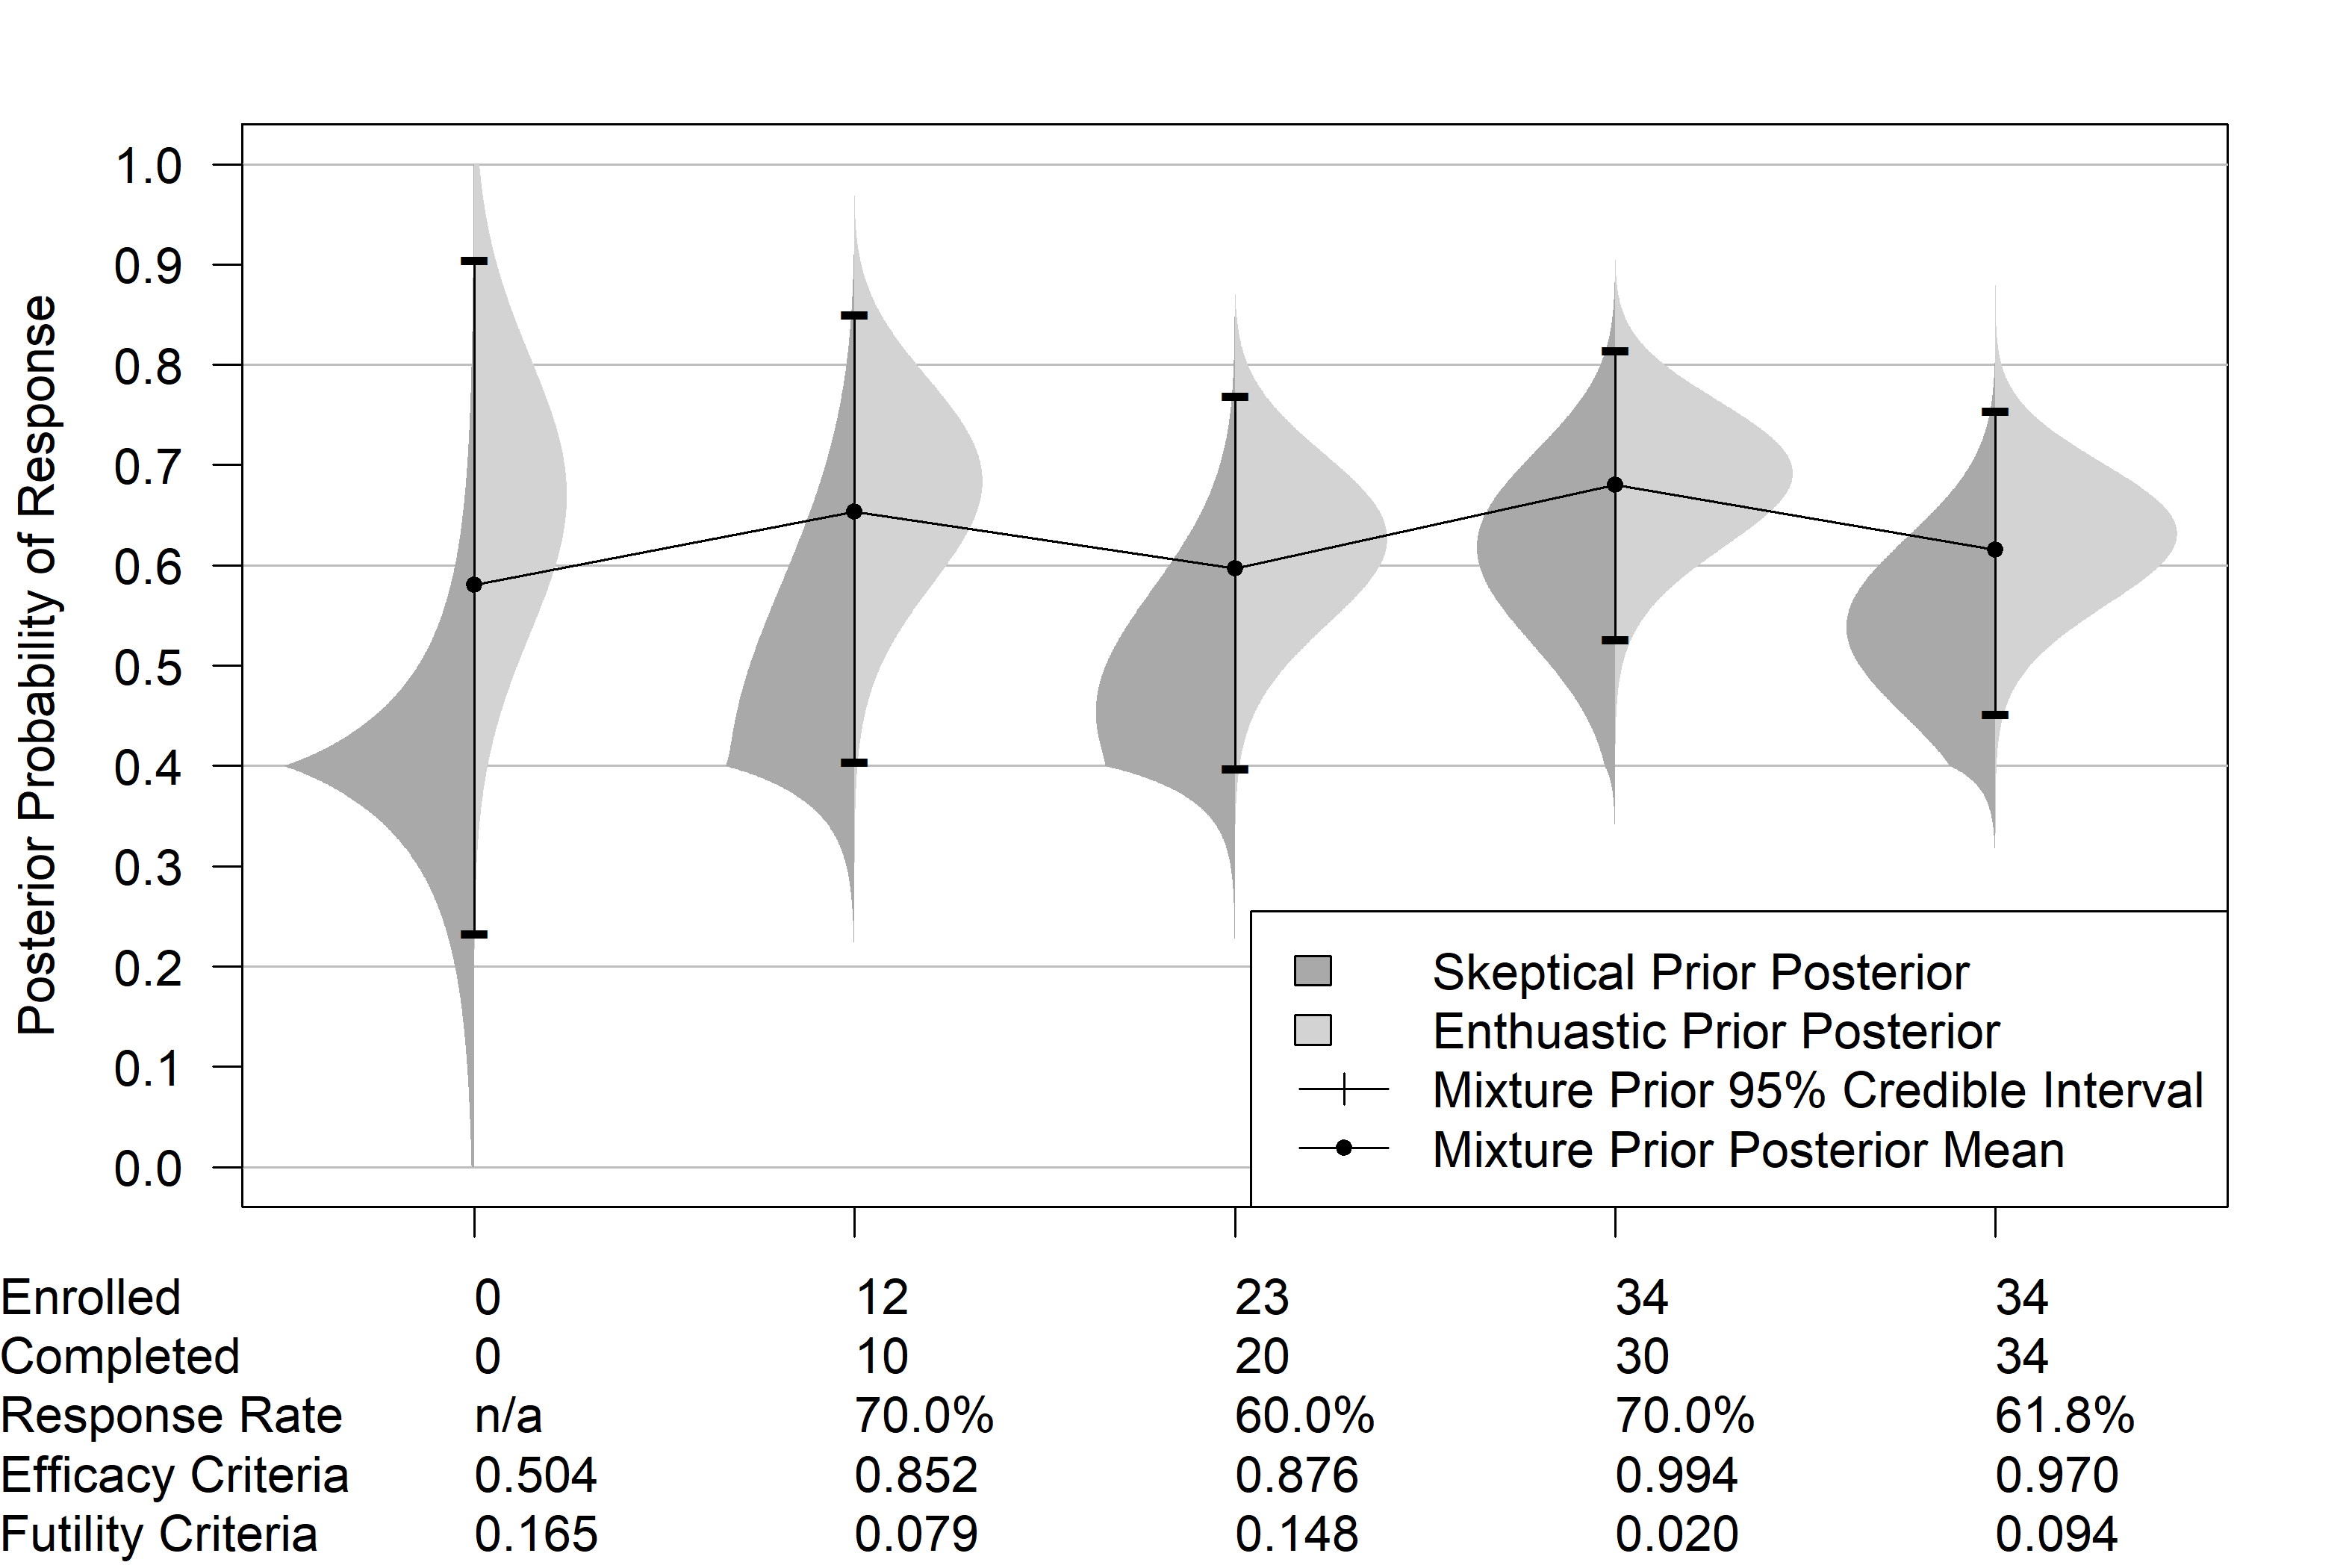
\includegraphics[width=6in]{figure2a.png}
    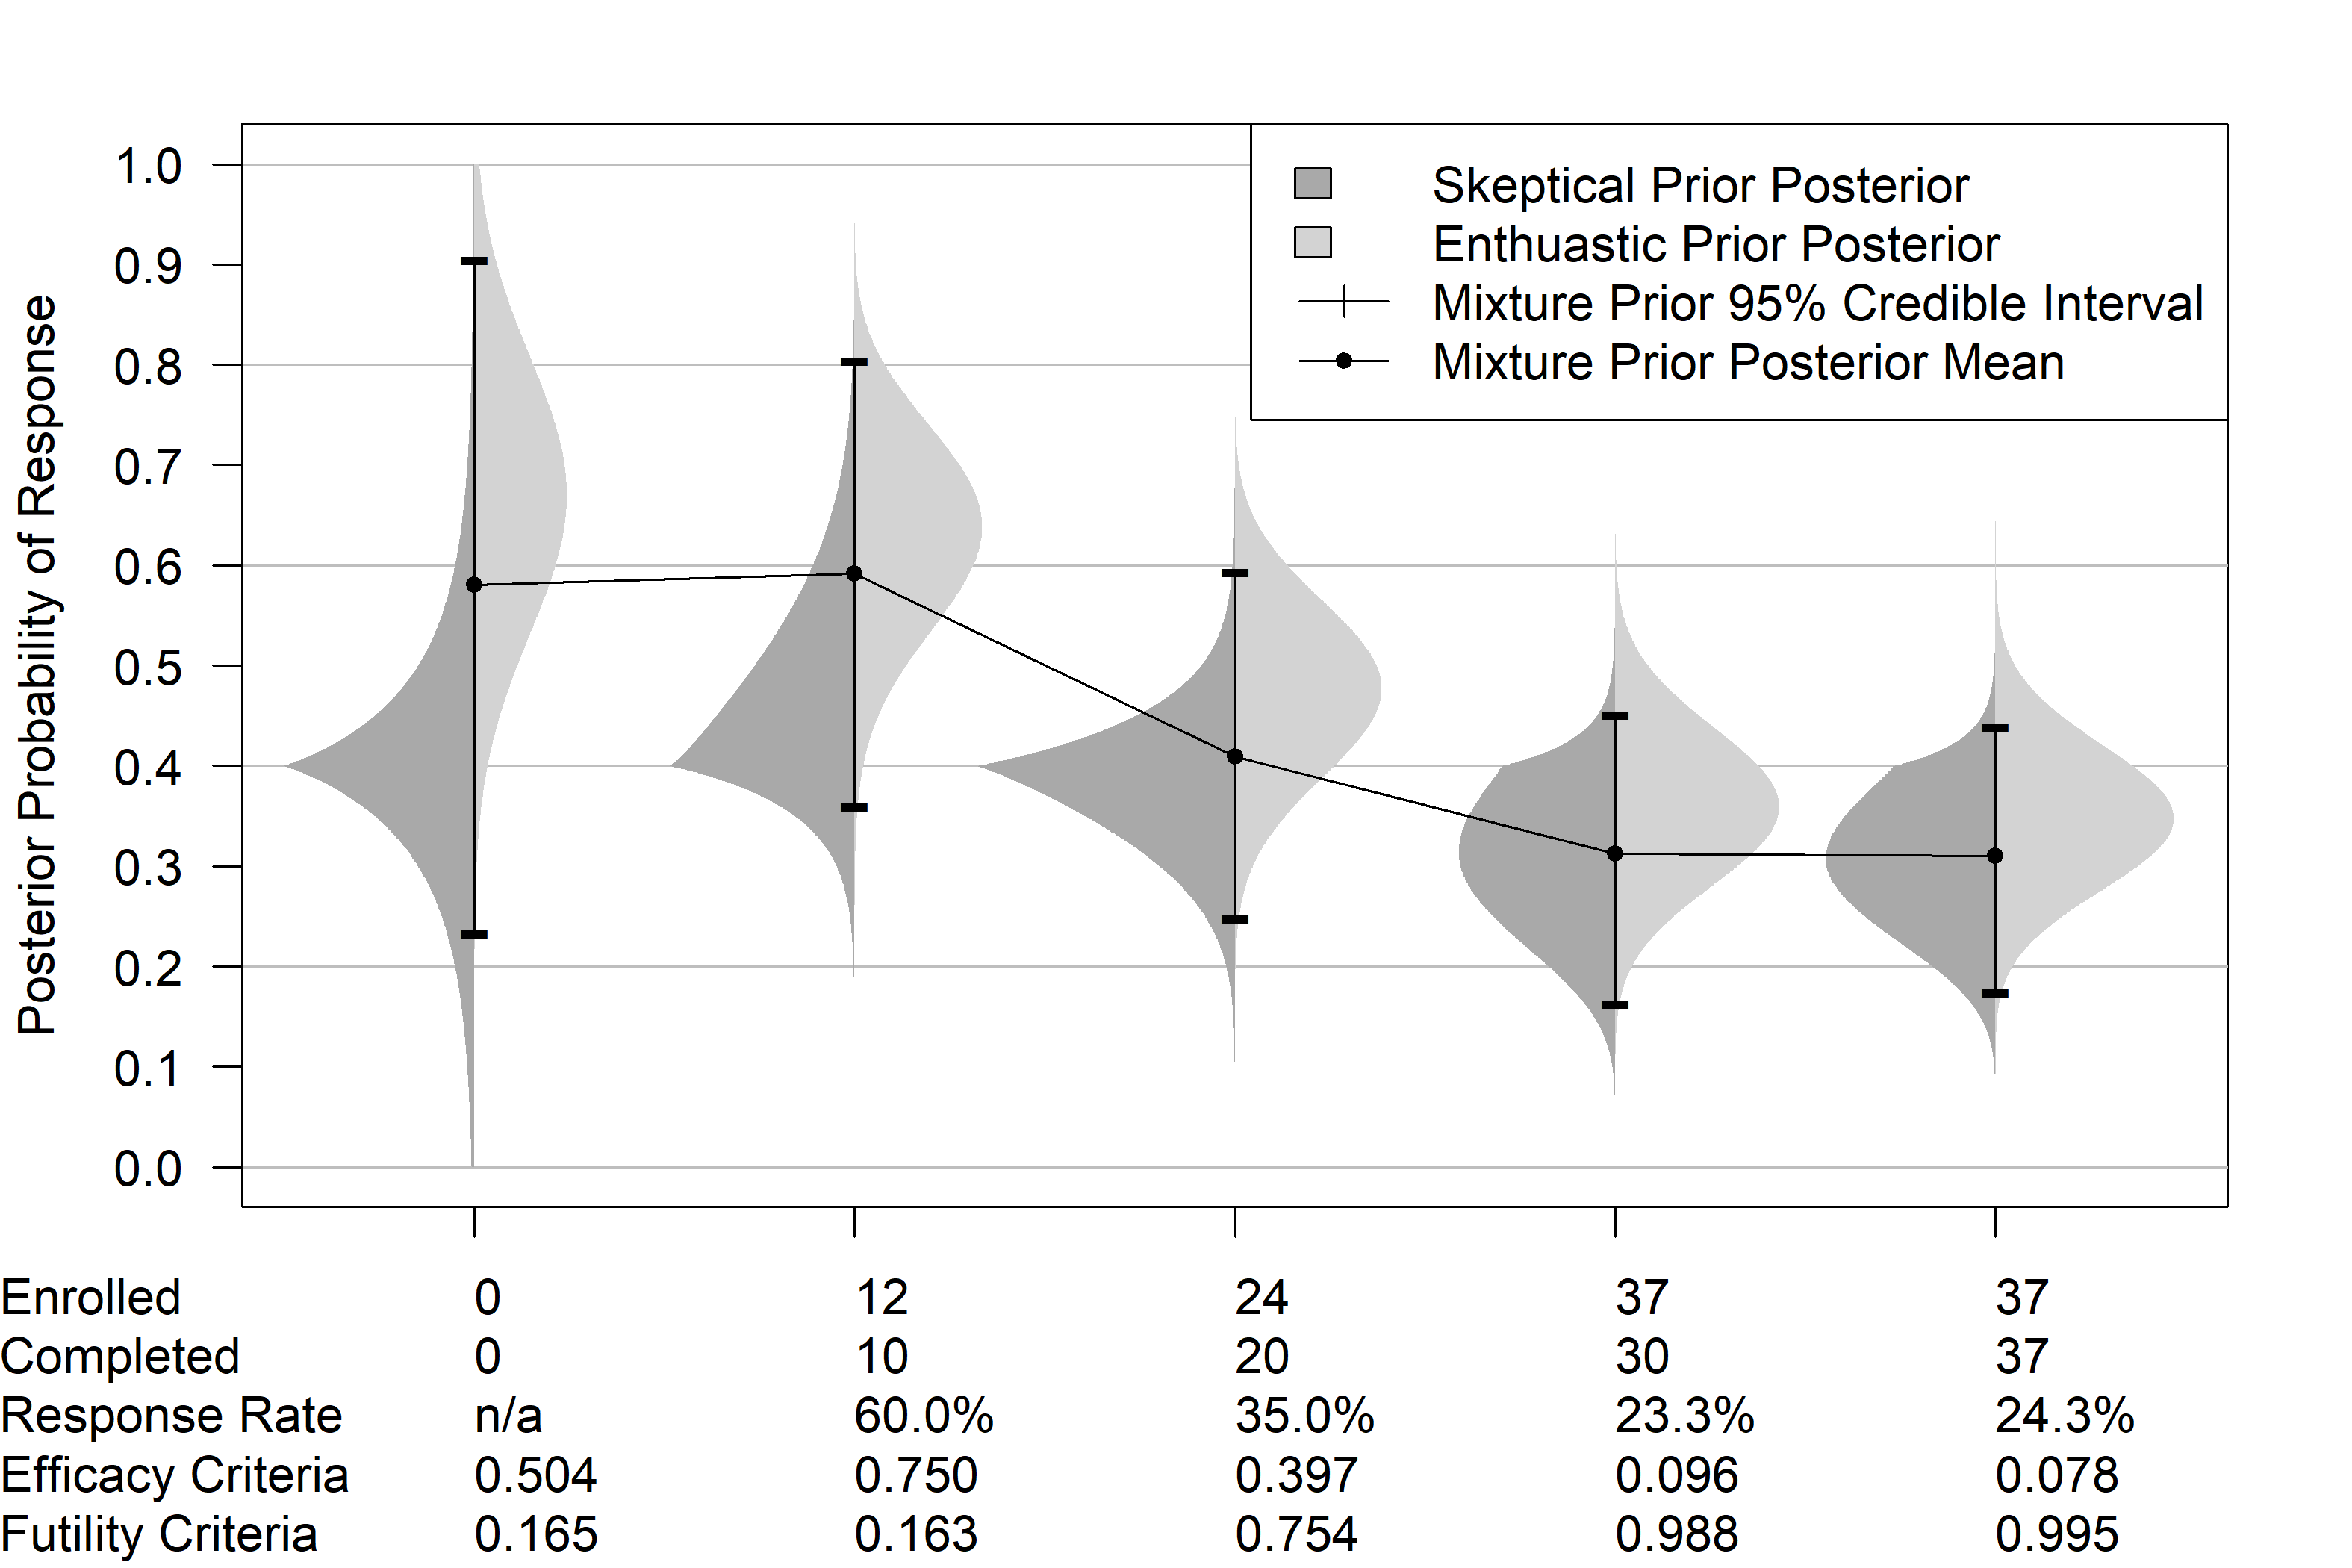
\includegraphics[width=6in]{figure2b.png}
    \caption{Example paths for the trial described in Section \ref{sec:example1model}. A, Early stoppage for efficacy. B, early stoppage for futility.}
	\label{fig:figure2}
\end{center}
\end{figure}

\subsection{Monitoring Prior Parameterization}
\subsubsection{Generalized Normal Distribution}\label{sec:gen_normal}
Skeptical and enthusiastic monitoring priors defined in Section \ref{sec:MP} have a required modal value and tail-probability constraint. There are many distributions which satisfy these conditions. The normal distribution will be used as a default choice. The specification of the mean and variance of a normal distribution completely specifies the modal value and tail-probability constraints, and is therefore sufficient for defining skeptical and enthusiastic priors (see Section \ref{sec:normal_tail_area}). Using a normal distribution as the monitoring prior is also motivated by the Bayesian Central Limit Theorem which states under general conditions that the posterior distribution for $\theta$ approaches normality as the sample size increases, regardless of the initial choice of prior. Therefore, a normally distributed monitoring prior is of the same family of distribution as a posterior which is the result of a large sample collection of data.

There is the possibility to change local behavior of the monitoring prior distribution around the modal value. The generalized normal distribution, which is an extension of the normal distribution, is able to change the local behavior around the modal value as compared to the default normally distributed monitoring prior, while still satisfying the modal value and tail probability constraints. The density for a generalized normal distribution $\mathcal{GN}(\mu,\alpha,\beta)$ is
$
f(\theta)=\frac{\beta}{2\alpha\Gamma(1/\beta)}\exp\{-(\frac{|\theta-\mu|}{\alpha})^\beta\}
$ where $\mu$ is a location parameter, $\alpha>0$ is a scale parameter, and $\beta>0$ is a shape parameter \citep{Nadarajah2005}. Fixing the location parameter to be the modal value and changing the shape and scale parameters in conjunction can maintain the tail probability constraint while also changing the behavior around the modal value (see Appendix Section \ref{sec:gen_normal_details}). A flattened monitoring is locally uniform around the modal value and a concentrated monitoring is peaked around the modal value. The flattened and concentrated priors have different levels of local dispersion around the modal value than what would be expected from a large sample collection of data according to the Bayesian Central Limit Theorem.

An example of flattened and concentrated enthusiastic priors are shown in Figure \ref{fig:figure1}. Choosing a flattened distribution is appropriate when $\theta$ is more likely to be in a wide range of values around $\theta_1$, while maintaining the same residual uncertainty that $\theta<\theta_0$. Choosing a concentrated distribution is appropriate when prior belief reflects a higher degree of certainty that $\theta$ is in a narrow range around $\theta_1$, while maintaining residual uncertainty that $\theta<\theta_0$. 
\begin{figure}
\begin{center}
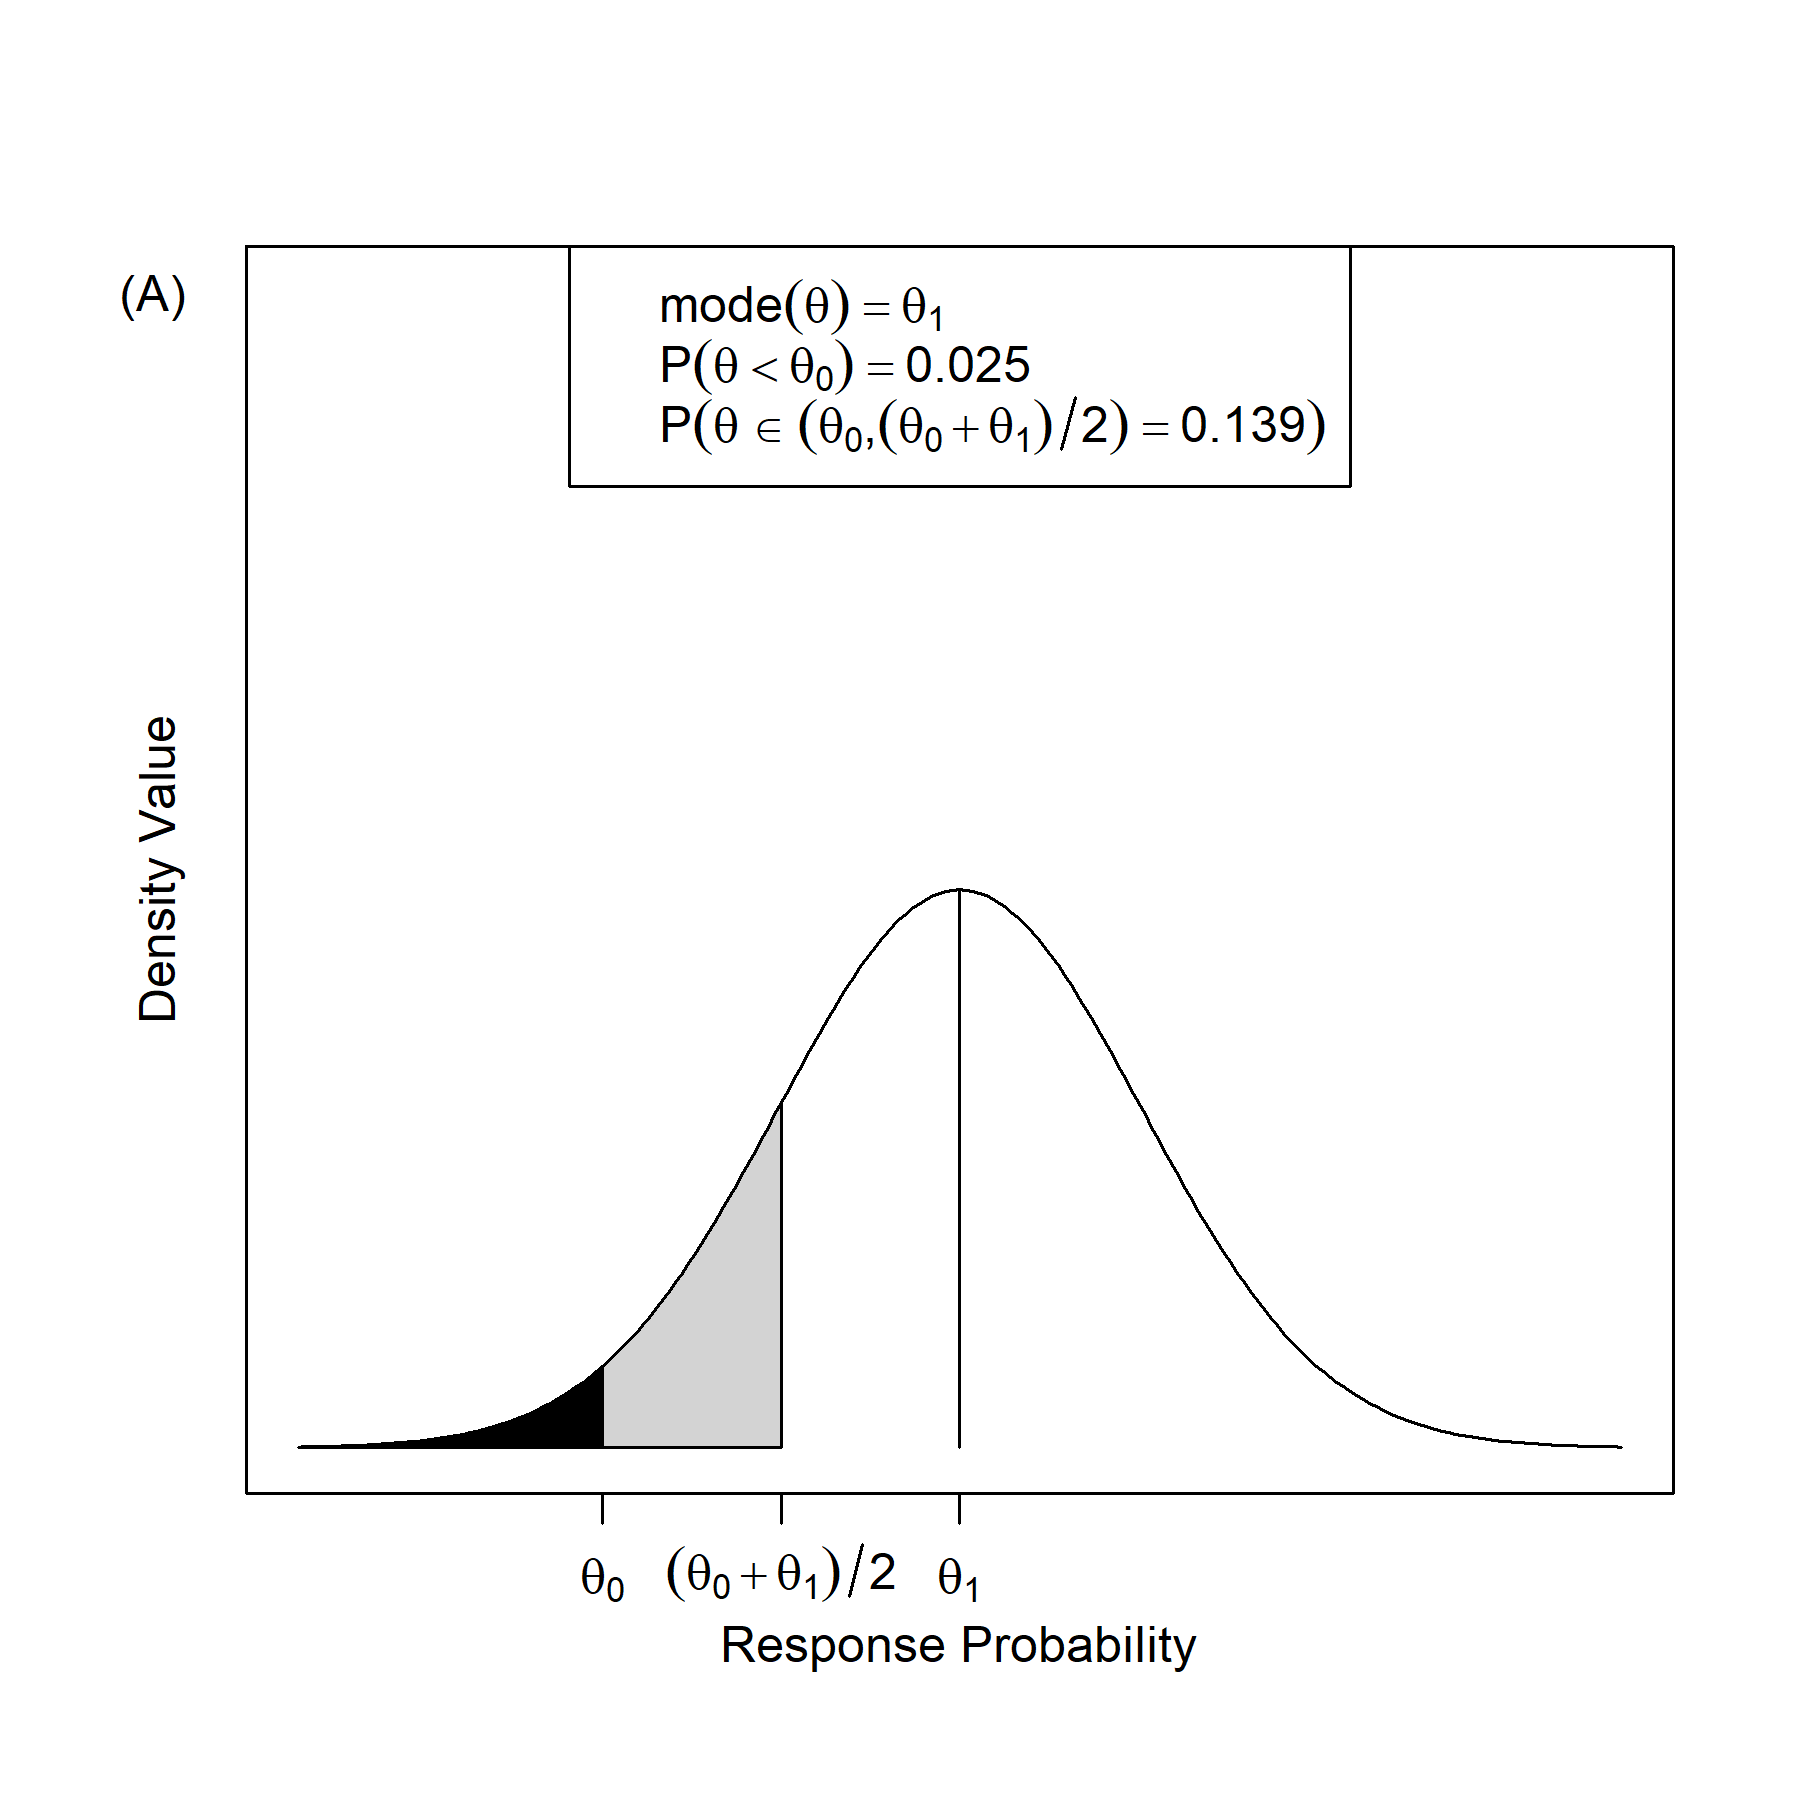
\includegraphics[width=3in]{figure1a.png}
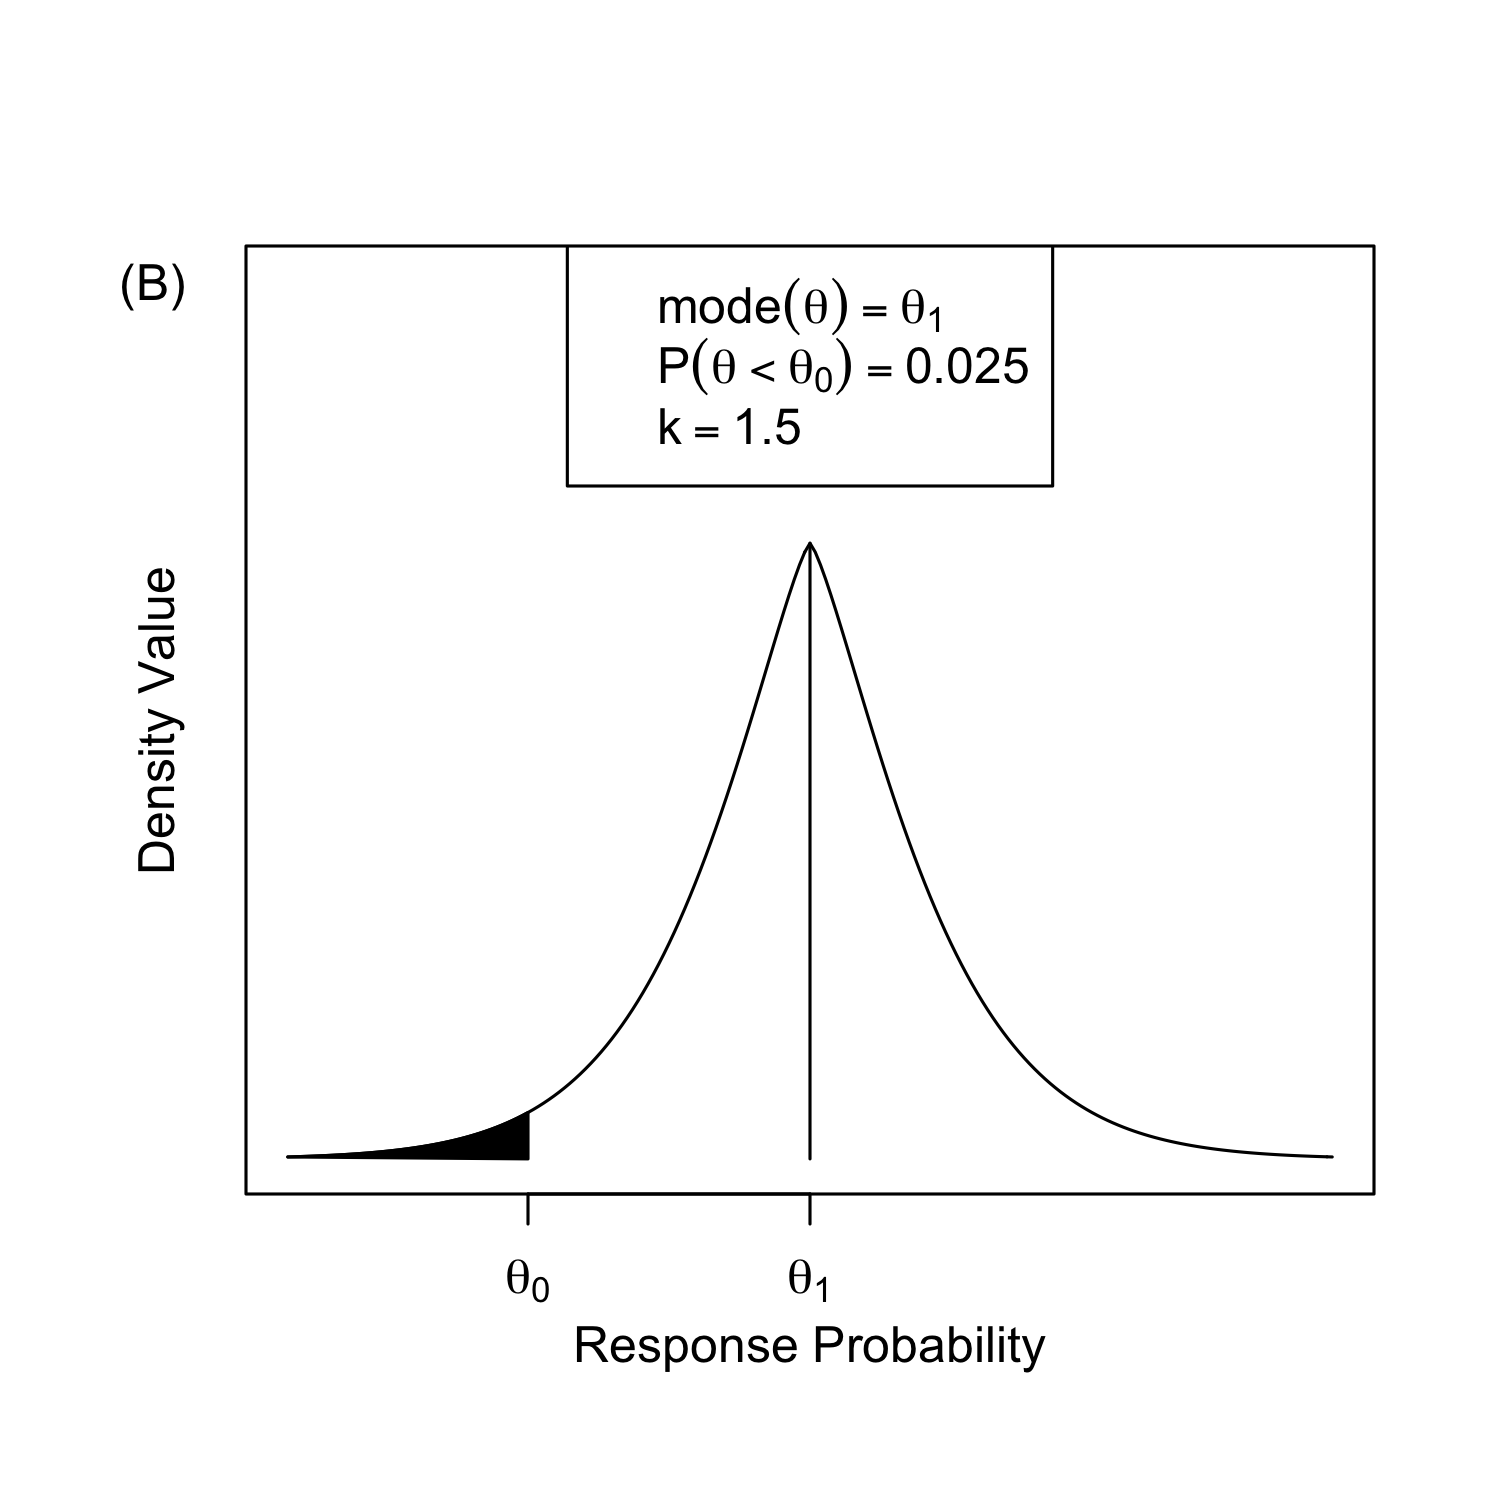
\includegraphics[width=3in]{figure1b.png}
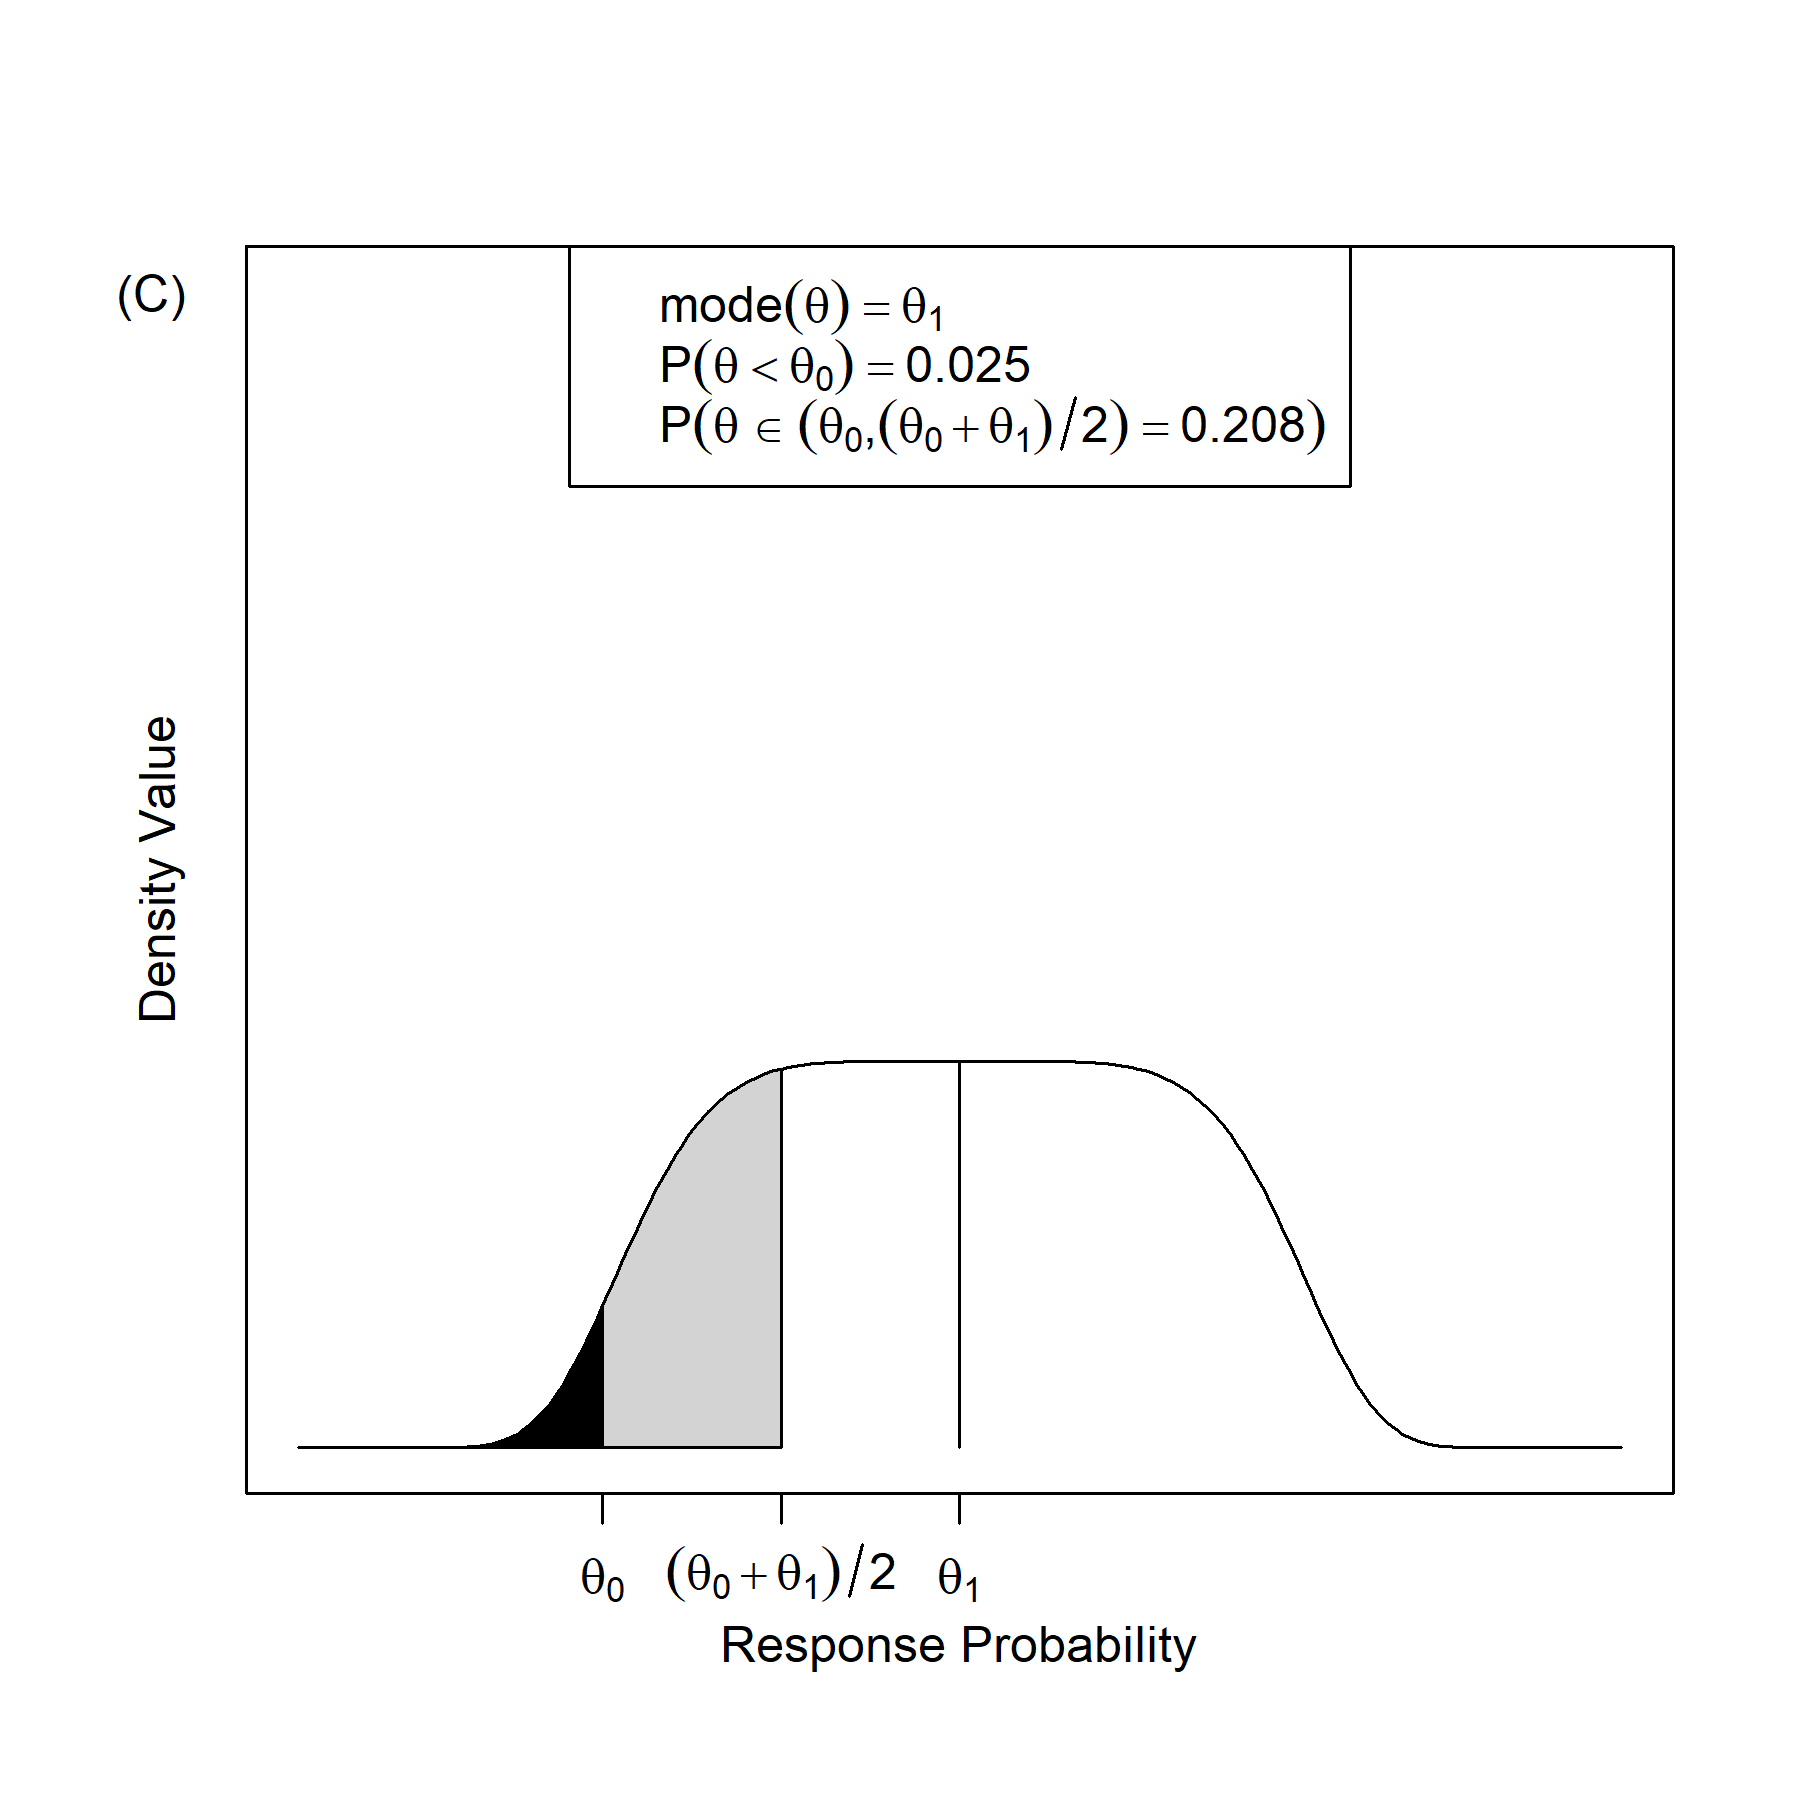
\includegraphics[width=3in]{figure1c.png}
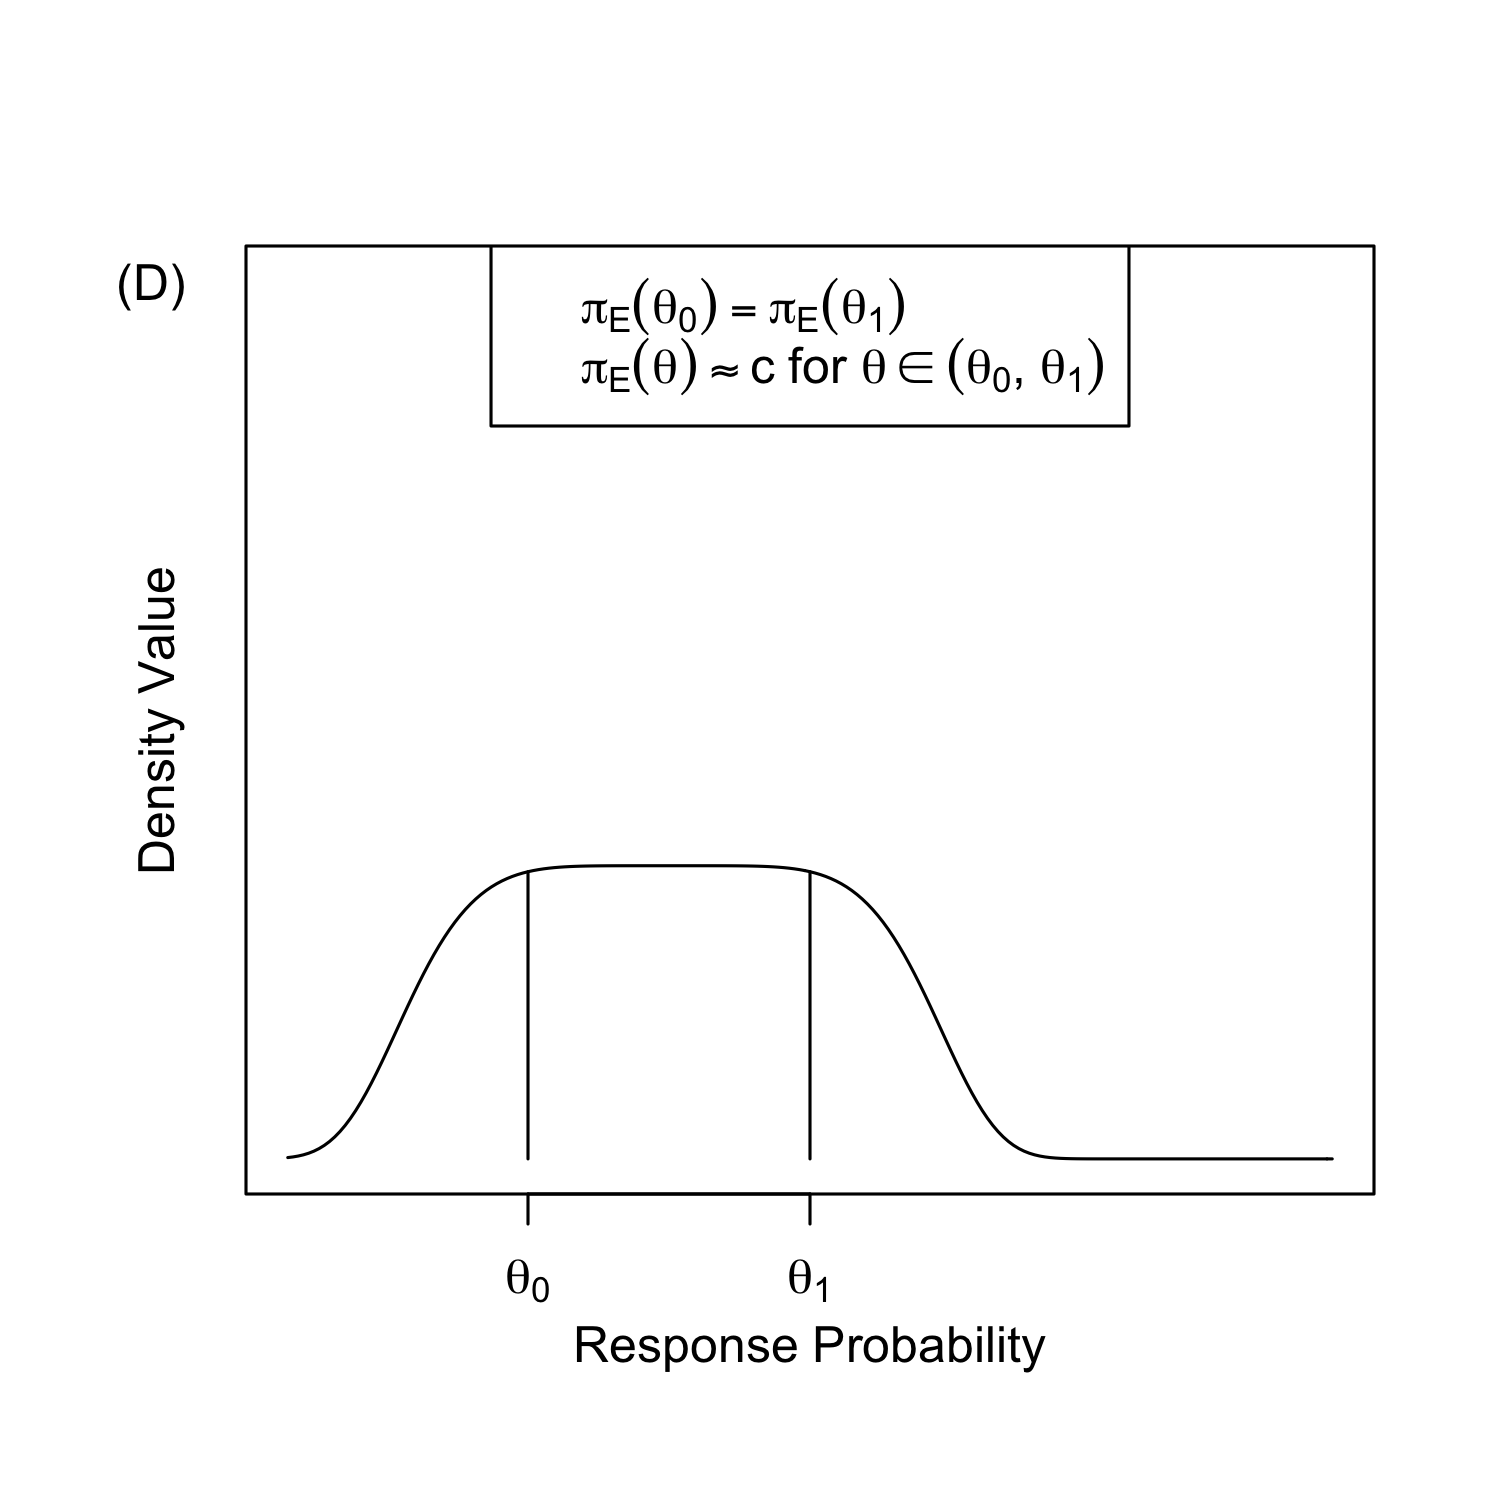
\includegraphics[width=3in]{figure1d.png}
\caption{A, Default enthusiastic prior. B, Concentrated enthusiastic prior. C, Flattened enthusiastic prior. D, Locally non-informative prior}

\label{fig:figure1}
\end{center}
\end{figure}
The flattened and enthusiastic priors will be parameterized by inflating or deflating the probability mass in the interval between $\theta_0$ and $\frac{\theta_0+\theta_1}{2}$ as compared to a normal distribution. The inflation/deflation of the area in this interval is shaded gray in Figure \ref{fig:figure1}. The flattened enthusiastic prior is defined as the generalized normal distribution that satisfies the modal value and tail probability constraints \eqref{eq:skptprior}-\eqref{eq:enthprior} that has 25\% less mass in the interval between $\theta_0$ and $\frac{\theta_0+\theta_1}{2}$ as compared to a normal distribution which satisfies the same modal value and tail probability constraints. Reducing the mass in this interval forces a peak around the modal value. Similarly, the flattened enthusiastic prior has 50\% more mass in the interval between $\theta_0$ and $\frac{\theta_0+\theta_1}{2}$, which forces a flattening around the modal value. These values of are chosen based on the intuitive graphical properties of the distribution (e.g. noticeably peaked around $\theta_1$, relatively flat around $\theta_1$). Likewise, a flattened skeptical prior has $25\%$ less mass in the interval between $\frac{\theta_0+\theta_1}{2}$ and $\theta_1$, and a concentrated skeptical prior as $50\%$ more mass in this same interval. These fixed inflation/deflation percentages provide for an unambiguous definition of a flattened or concentrated prior (see technical definition in Section \ref{sec:gen_norm_appendix}). There are other inflation/deflation percentages which would achieve the same purpose, but these values will be used henceforth to demonstrate the concepts. Alternatively, the choice of shape and scale parameters could be specified to identify an additional probability constraint exactly (e.g. $P(\theta\in(\theta_0,\frac{\theta_0+\theta_1}{2}))=0.1$). The default, flattened, and concentrated priors can all be truncated while maintaining the mode and tail probability constraints.

A locally non-informative prior is a prior that is relatively flat over a wide range of plausible values of $\theta$ (in particular, relatively flat over the interval $(\theta_0,\theta_1))$. The locally non-informative prior can be viewed as a particular case of the enthusiastic prior. Define a locally non-informative prior $\pi_{NI}(\theta)$ as a prior that suggests $\frac{\theta_0+\theta_1}{2}$ is the most likely value of $\theta$ and that reflects the belief of an observer who is \textit{all but convinced} that $\theta>\frac{\theta_0+\theta_1}{2}-2(\theta_1-\theta_0)=\frac{3\theta_0-\theta_1}{2}$ a priori. Formally, this is defined as the prior $\pi_{NI}(\theta)$ satisfying
\begin{equation}\label{eq:niprior}
argmax_\theta P_{NI}(\theta)=\frac{\theta_0+\theta_1}{2}\text{ and } P_{NI}(\theta<\frac{3\theta_0-\theta_1}{2})=1-\epsilon.
\end{equation}
This prior will be flattened such that there is $50\%$ more mass in the interval $(\frac{3\theta_0-\theta_1}{2},\theta_0)$ as compared to a normal distribution with the same modal value and tail probability constraint. The locally non-informative prior is shown in Figure \ref{fig:figure1}, and the technical definition is in Section \ref{sec:gen_norm_appendix}.
%\item If $\gamma>1$ then the probability that $\theta\in(q,\frac{q+\mu}{2})$ increases and the concentration of $\theta$ around the modal value $\mu$ accordingly decreases, resulting in a flatter distribution around the modal value. 
%\item If $\gamma<1$ then the probability that $\theta\in(q,\frac{q+\mu}{2})$ decreases and the concentration of $\theta$ around the modal value $\mu$ accordingly increases, resulting in a more concentrated distribution around the modal value. 
%\item Flattening or concentrating the distribution around the modal value is useful for specifying monitoring priors that reflect varying opinions about the dispersion of $\theta$. 
%\item An example of parameterizing an enthusiastic prior with a $\mathcal{GN}_p(\tilde{\mu},q,\gamma)$ distribution is demonstrated in Figure \ref{fig:figure1}. 
%\item Choosing a concentrated distribution is appropriate when prior belief reflects a higher degree of certainty that $\theta$ is in a narrow range around $\theta_1$, while maintaining residual uncertainty that $\theta<\theta_0$. 
%\item This decreases the variance of the distribution, and can be seen to reflect a conservative opinion about the values of $\theta$. 
%\item Choosing a flattened distribution is appropriate when $\theta$ is more likely to be in a wide range of values around $\theta_1$, while maintaining the same residual uncertainty that $\theta<\theta_0$. 
%\item This increases the variance of the distribution, and can be seen to reflect a liberal opinion about the values of $\theta$. 

%\item The impact of flattening or concentrating the distribution of a monitoring prior on the operating characteristics of a trial is shown in Section \ref{sec:examples}.
%For example, consider creating skeptical and enthusiastic priors for a response probability on domain $[0,1]$, as $
%\pi_S(\theta)=\mathcal{GN}_{p=1-\epsilon,\Theta=[0,1]}(\tilde{\mu}=\theta_0,q=\theta_1,\gamma=1)$ and $
%\pi_E(\theta)=\mathcal{GN}_{p=\epsilon,\Theta=[0,1]}(\tilde{\mu}=\theta_1,q=\theta_0,\gamma=1)$ respectively.

%The normal and generalized normal family of distributions can be truncated to a restricted domain that reflects the research quantity of interest (e.g. a response probability on [0,1]).
%\subsubsection{Application to higher dimensions}
%Suppose the trial from Section \ref{sec:preliminaries} has added a control arm, and let $\eta_0$ and $\eta_1$ be the response proportions for a control and treatment group respectively. Suppose that the risk difference $\theta=\eta_1-\eta_0$ is the parameter of interest, and let $\eta_0$ be a nuisance parameter. Let $\delta_0$ denote a null risk difference and $\delta_1$ denote a highly efficacious risk difference.

\subsubsection{Incorporating Prior Information in the Monitoring Priors}\label{sec:incorporating}
Prior information can be incorporated into the monitoring priors resulting in a mixture distribution with mixing weight $\omega$ of the form
\begin{equation}\label{eq:inference_prior}
\pi\left(\theta\right)=\omega\cdot\pi_{S}\left(\theta\right)+(1-\omega) \cdot \pi_E\left(\theta\right),
\end{equation}
where $\omega\in[0,1]$. 

The mixing weight $\omega$ is determined by an assessment of prior-data conflict using the prior predictive distribution of the data \citep{Box1980}.
The prior-predictive distribution of the data gives the probability of future observations of the data given initial assumptions about $\theta$, and is defined as
\begin{equation}\label{eq:pred_dist}
p(\mathbf{D})=\int \mathcal{L}(\theta|\mathbf{D})\pi(\theta)d\theta
\end{equation}

Let $\mathbf{D}_{\text{obs}}$ be the observed data at some point in time. For each predictive density, we compute the following:
%\begin{equation}
%p=P(p(y)\leq p(y_{obs}))
%\end{equation}
\begin{equation}\label{eq:box_p}
\psi(\mathbf{D})=\int 1[p(\mathbf{D})\leq p(\mathbf{D}_{\text{obs}})] d(\mathbf{D})
%\sum_{\mathbf{D}}p^{(h)}(\mathbf{D})1[p^{(h)}(\mathbf{D})\leq p^{(h)}(\mathbf{D}_{\text{obs}})]
\end{equation}
which in the case of discrete data is equal to $\psi(\mathbf{D})=\sum_{\mathbf{D}}p(\mathbf{D})1[p(\mathbf{D})\leq p(\mathbf{D}_{\text{obs}})]$.
This can be interpreted as the probability of observing data as or more extreme given the predictive distribution. Small values of $\psi(\mathbf{D})$ indicate inconsistency between the prior and the data. 

The skeptical and enthusiastic priors $\pi_S(\theta)$ and $\pi_E(\theta)$ will be used in \eqref{eq:pred_dist} and \eqref{eq:box_p} to create compatibility measurements $\psi^{(S)}(\mathbf{D})$ and $\psi^{(E)}(\mathbf{D})$ which will be used to determine the mixing weight in \eqref{eq:inference_prior}. If $\psi^{(E)}(\mathbf{D})>\psi^{(S)}(\mathbf{D})$, then the data are more consistent with the enthusiastic prior, which should be given a greater weight in the mixture. Similarly, if $\psi^{(S)}(\mathbf{D})>\psi^{(E)}(\mathbf{D})$ then the skeptical prior should be given a greater mixing weight.

A conservative choice of mixing weight which gives full weight to the skeptical prior (i.e. $\omega=1$) whenever $\psi^{(S)}(\mathbf{D})\geq \psi^{(E)}(\mathbf{D})$ is
\begin{equation}\label{eq:adaptive_prior}
\omega=\begin{cases} 
      1 & \text{if } \psi^{(S)}(\mathbf{D})\geq \psi^{(E)}(\mathbf{D}) \\
      1-(\psi^{(E)}(\mathbf{D})-\psi^{(S)}(\mathbf{D})) &\text{if } \psi^{(S)}(\mathbf{D})< \psi^{(E)}(\mathbf{D}
   \end{cases}
\end{equation}
The weight given to the enthusiastic prior is $\psi^{(E)}(\mathbf{D})-\psi^{(S)}(\mathbf{D})$ which is equal to how much more the data is compatible with the enthusiastic prior than it is the skeptical prior.
%
%Bayesian predictive model checking: model checking statistic and reference predictive distribution.




%

%


%Alternatively, $\omega$ can be informed by the data. Let $\hat{\theta}=\rmn{argmax} \{p(\bmath{D}|\theta)\}$ be the maximum likelihood estimator of $\theta$ given the data.
%%
%%%\begin{mydef}
%Define
%\begin{equation}\label{eq:dynamic_omega}
%\omega=\omega_{min}+(1-\omega_{min})\frac{\pi_S(\hat{\theta})}{\pi_S(\hat{\theta})+\pi_E(\hat{\theta})}
%\end{equation}
%as a mixing weight that dynamically gives preference to the prior that has the higher density evaluated at $\hat{\theta}$ with a minimum weight $\omega_{min}$ given to the skeptical component with $\omega_{min}\in[0,1]$.
%%%\end{mydef}

\subsubsection{Mixture Inference Prior}
The purpose of the inference prior is to synthesize the posterior inferences from the a priori diverse perspectives to facilitate interpretation of the data once it has been obtained. The skeptical and enthusiastic monitoring priors defined in Section~\ref{sec:MP} represent extreme but plausible beliefs about $\theta$.
%
While analysis with these priors provides a rational perspective from which one can determine whether interim data are sufficient 
to cease enrolling patients, the a priori belief of most stakeholders will likely fall somewhere in between the two perspectives.
%
Thus, when interpreting the final data once in hand, intermediate perspectives should be considered.
%
To that end, we define an inference prior as a mixture prior constructed by mixing the monitoring priors.

Using the mixture prior specification of \eqref{eq:inference_prior}, a fixed value of $\omega=1/2$ will be referred to as an agnostic inference prior since it gives equal weight to the skeptical and enthusiastic prior.

The inference prior can also be determined based on an assessment of prior-data conflict. Let $\pi_{NI}(\theta)$ denote a locally non-informative prior that is relatively flat over plausible values of $\theta$. Consider a three-part mixture prior
\begin{equation}\label{eq:3partmix}
\pi(\theta)=\omega_S\cdot \pi_S(\theta)+\omega_E\cdot\pi_E(\theta)+\omega_{NI}\cdot\pi_{NI}(\theta)
\end{equation}
where $\omega_S+\omega_E+\omega_{NI}=1$. The quantities $\psi^{(E)}$, $\psi^{(S)}$, and $\psi^{(NI)}$ will be derived from using the priors $\pi_S(\theta)$, $\pi_E(\theta)$, and $\pi_{NI}(\theta)$ in the expression for Box's p-value \eqref{eq:box_p}. Each of $\psi^{(E)}$, $\psi^{(S)}$, and $\psi^{(NI)}$ represent compatibility of the data with the prior. 

Our goal is to create a mixture prior which favors the skeptical or enthusiastic components in areas where high compatibility is demonstrated for those components, and favors the locally non-informative prior if both the skeptical and enthusiastic components show low compatibility. To this end, consider transforming $\psi^{(NI)}$ to
\begin{equation}\label{eq:3partmix_ni}
\tilde{\psi}^{(NI)}=\begin{cases} 
      \psi^{(NI)}-\text{max}(\psi^{(S)},\psi^{(E)}) &\text{ if } \psi^{(NI)}>\text{max}(\psi^{(S)},\psi^{(E)})\\
      0& \text{ if } \psi^{(NI)}\leq\text{max}(\psi^{(S)},\psi^{(E)})
   \end{cases}
\end{equation}

Then let the mixing weights $\omega^{(E)}$, $\omega^{(S)}$, and $\omega^{(NI)}$ be the normalized values of $\psi^{(E)}$, $\psi^{(S)}$, and $\tilde{\psi}^{(NI)}$ so that their sum is unity (e.g. $\omega^{(E)}=\psi^{(E)}/(\psi^{(E)}+\psi^{(S)}+\tilde{\psi}^{(NI)}))$. This type of inference prior is used in Section \ref{sec:example2}.

%
%The posterior distribution for $\theta$ using \eqref{eq:inference_prior} is
%\begin{equation}
%p(\theta|\bmath{D},\pi_I)=\hat{\omega}\cdot p(\theta|\bmath{D},\pi_S)+(1-\hat{\omega})\cdot p(\theta|\bmath{D},\pi_E)
%\end{equation}
%where the updated mixing weight is
%\begin{equation}
%\hat{\omega}=\frac{\omega\cdot p(\bmath{D}|\pi_S)}{\omega\cdot p(\bmath{D}|\pi_S)+(1-\omega)\cdot p(\bmath{D}|\pi_E)}
%\end{equation}
%where $p(\bmath{D}|\pi_S)=\int p(\bmath{D}|\theta)\pi_S(\theta)d\theta$ and $p(\bmath{D}|\pi_E)=\int p(\bmath{D}|\theta)\pi_S(\theta)d\theta$. 

\subsubsection{Marginal-Conditional Specification}\label{sec:cond_marg}
In the case of nuisance parameters, marginal-conditional factorization of the joint prior $\pi(\theta,\eta)$ will be used. Let $\theta$ be the parameter of interest and $\eta$ be the nuisance parameters. Consider the following representation of the joint prior for $\theta$ and $\eta$: $\pi(\theta,\eta)=\pi(\theta)\times\pi(\eta|\theta)$. Then priors for both $\pi(\theta)$ and $\pi(\eta|\theta)$ will be given that satisfy the modal value and tail probability constraints \eqref{eq:skptprior}-\eqref{eq:enthprior} (see details in Section \ref{sec:gen_norm_appendix}). For example, suppose that $\theta$ is the risk difference between response probabilities of the treatment group and the placebo group, and denote the  probability of the placebo group by $\eta$. This prior specification is demonstrated in Figure \ref{fig:figure5}, and Section \ref{sec:example2model} uses this representation of the joint prior.

\begin{figure}\begin{center}
%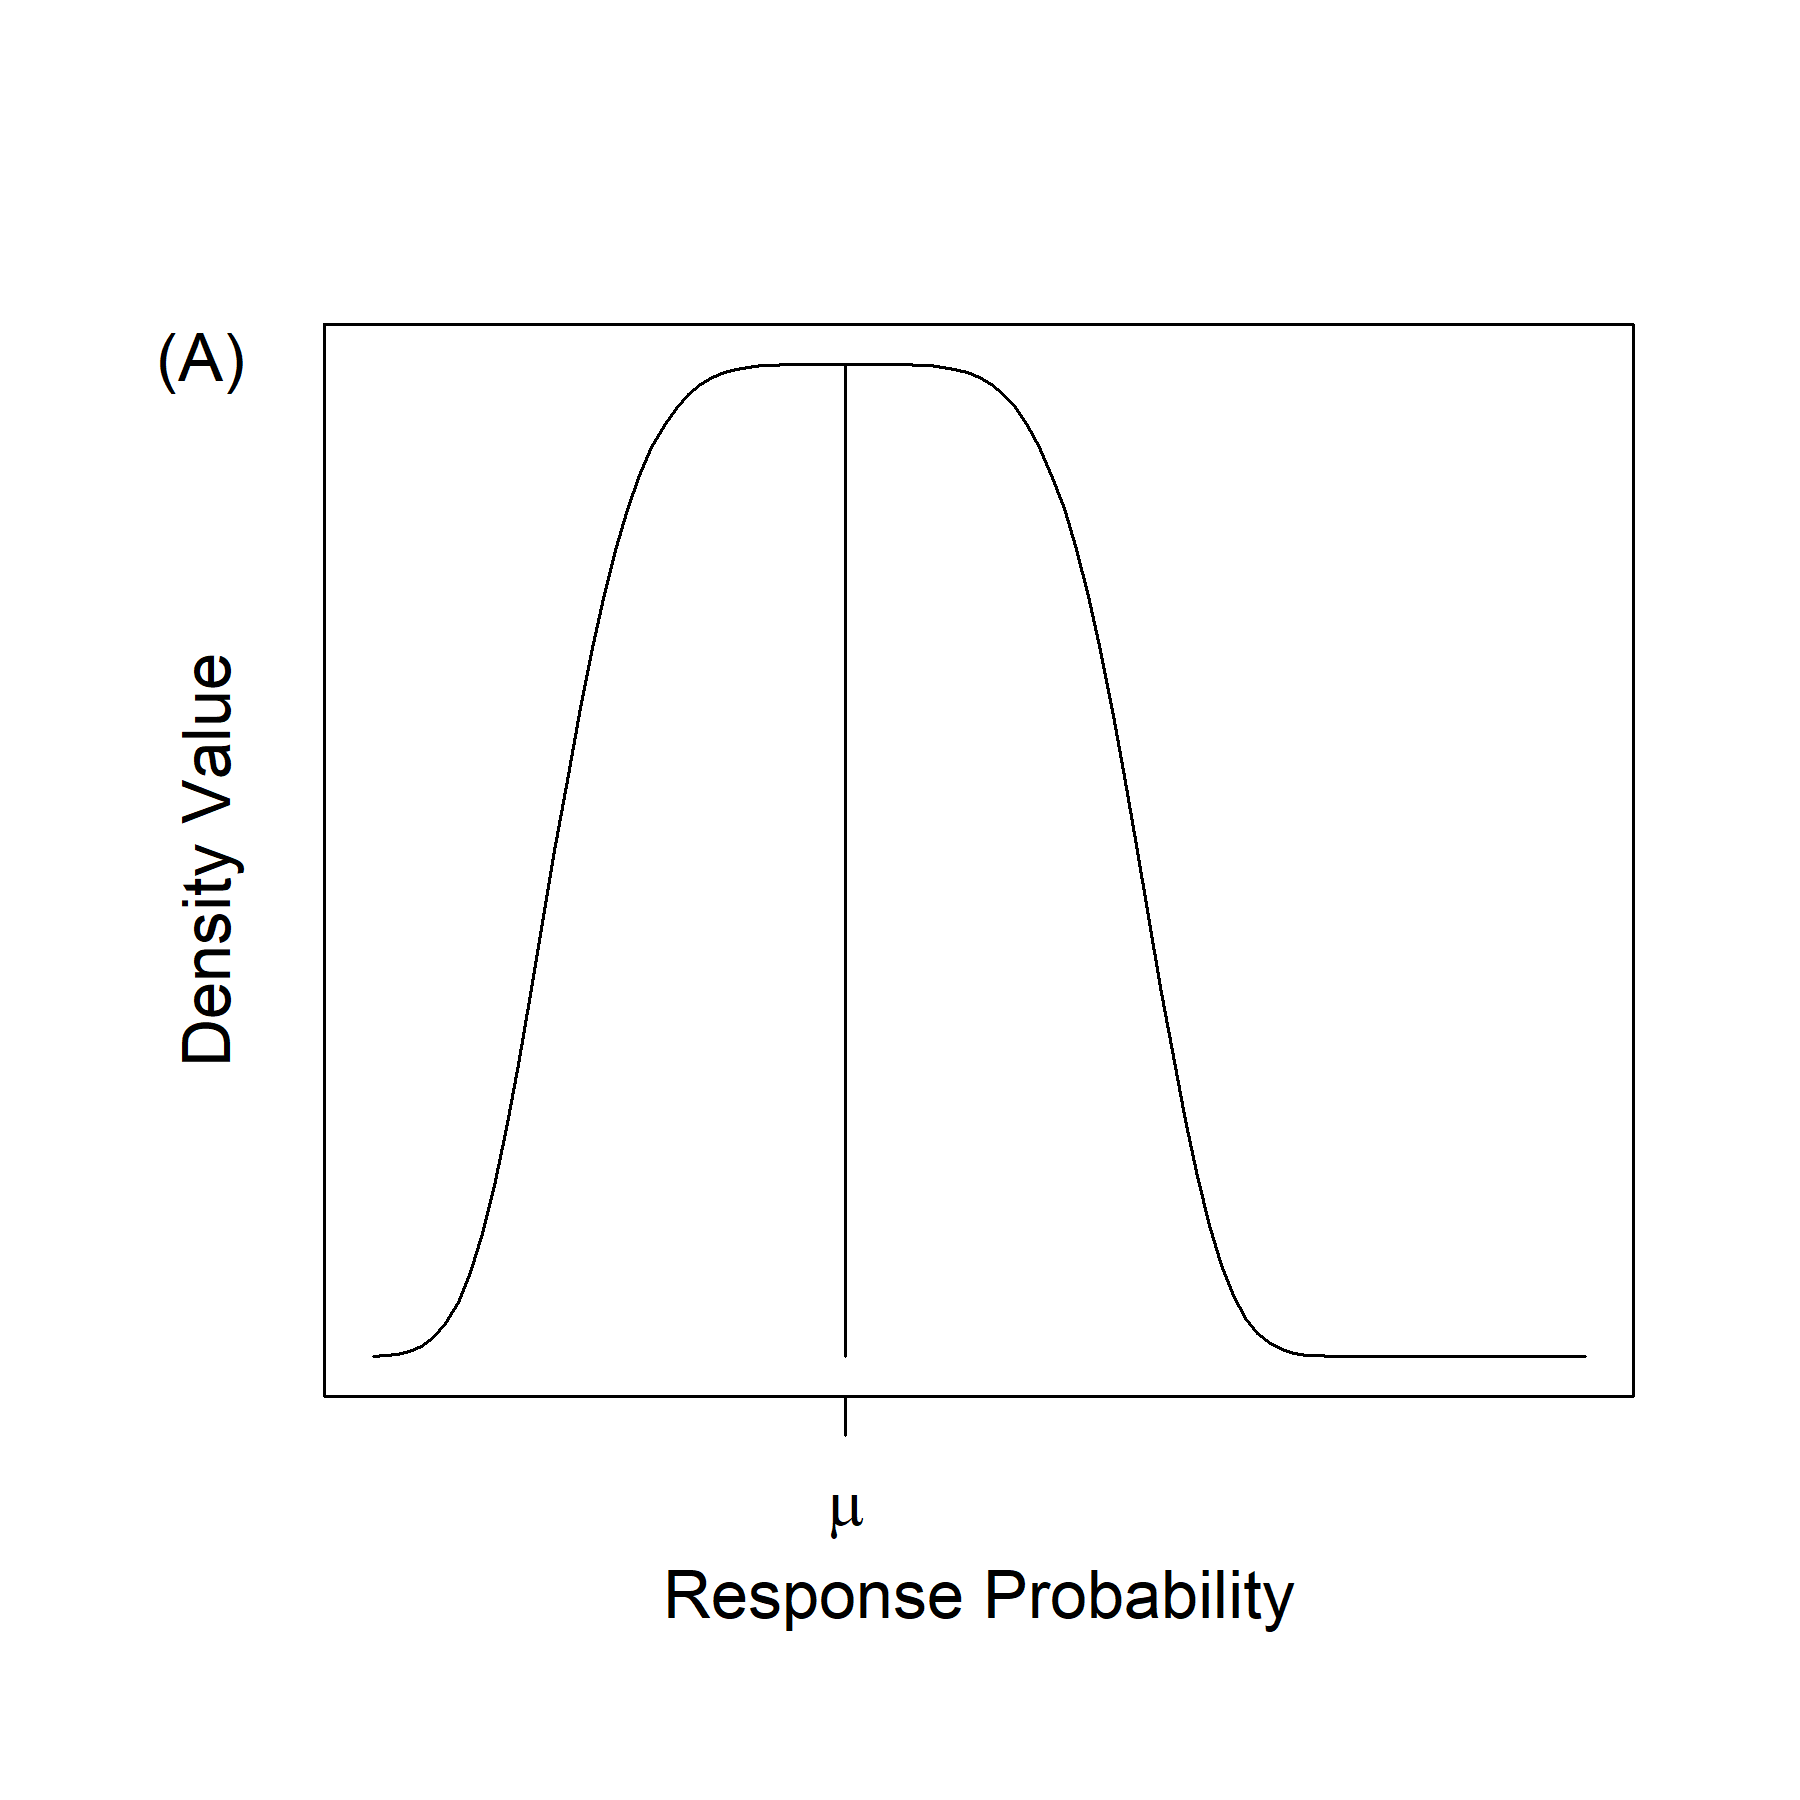
\includegraphics[width=6in]{figure5c.png}
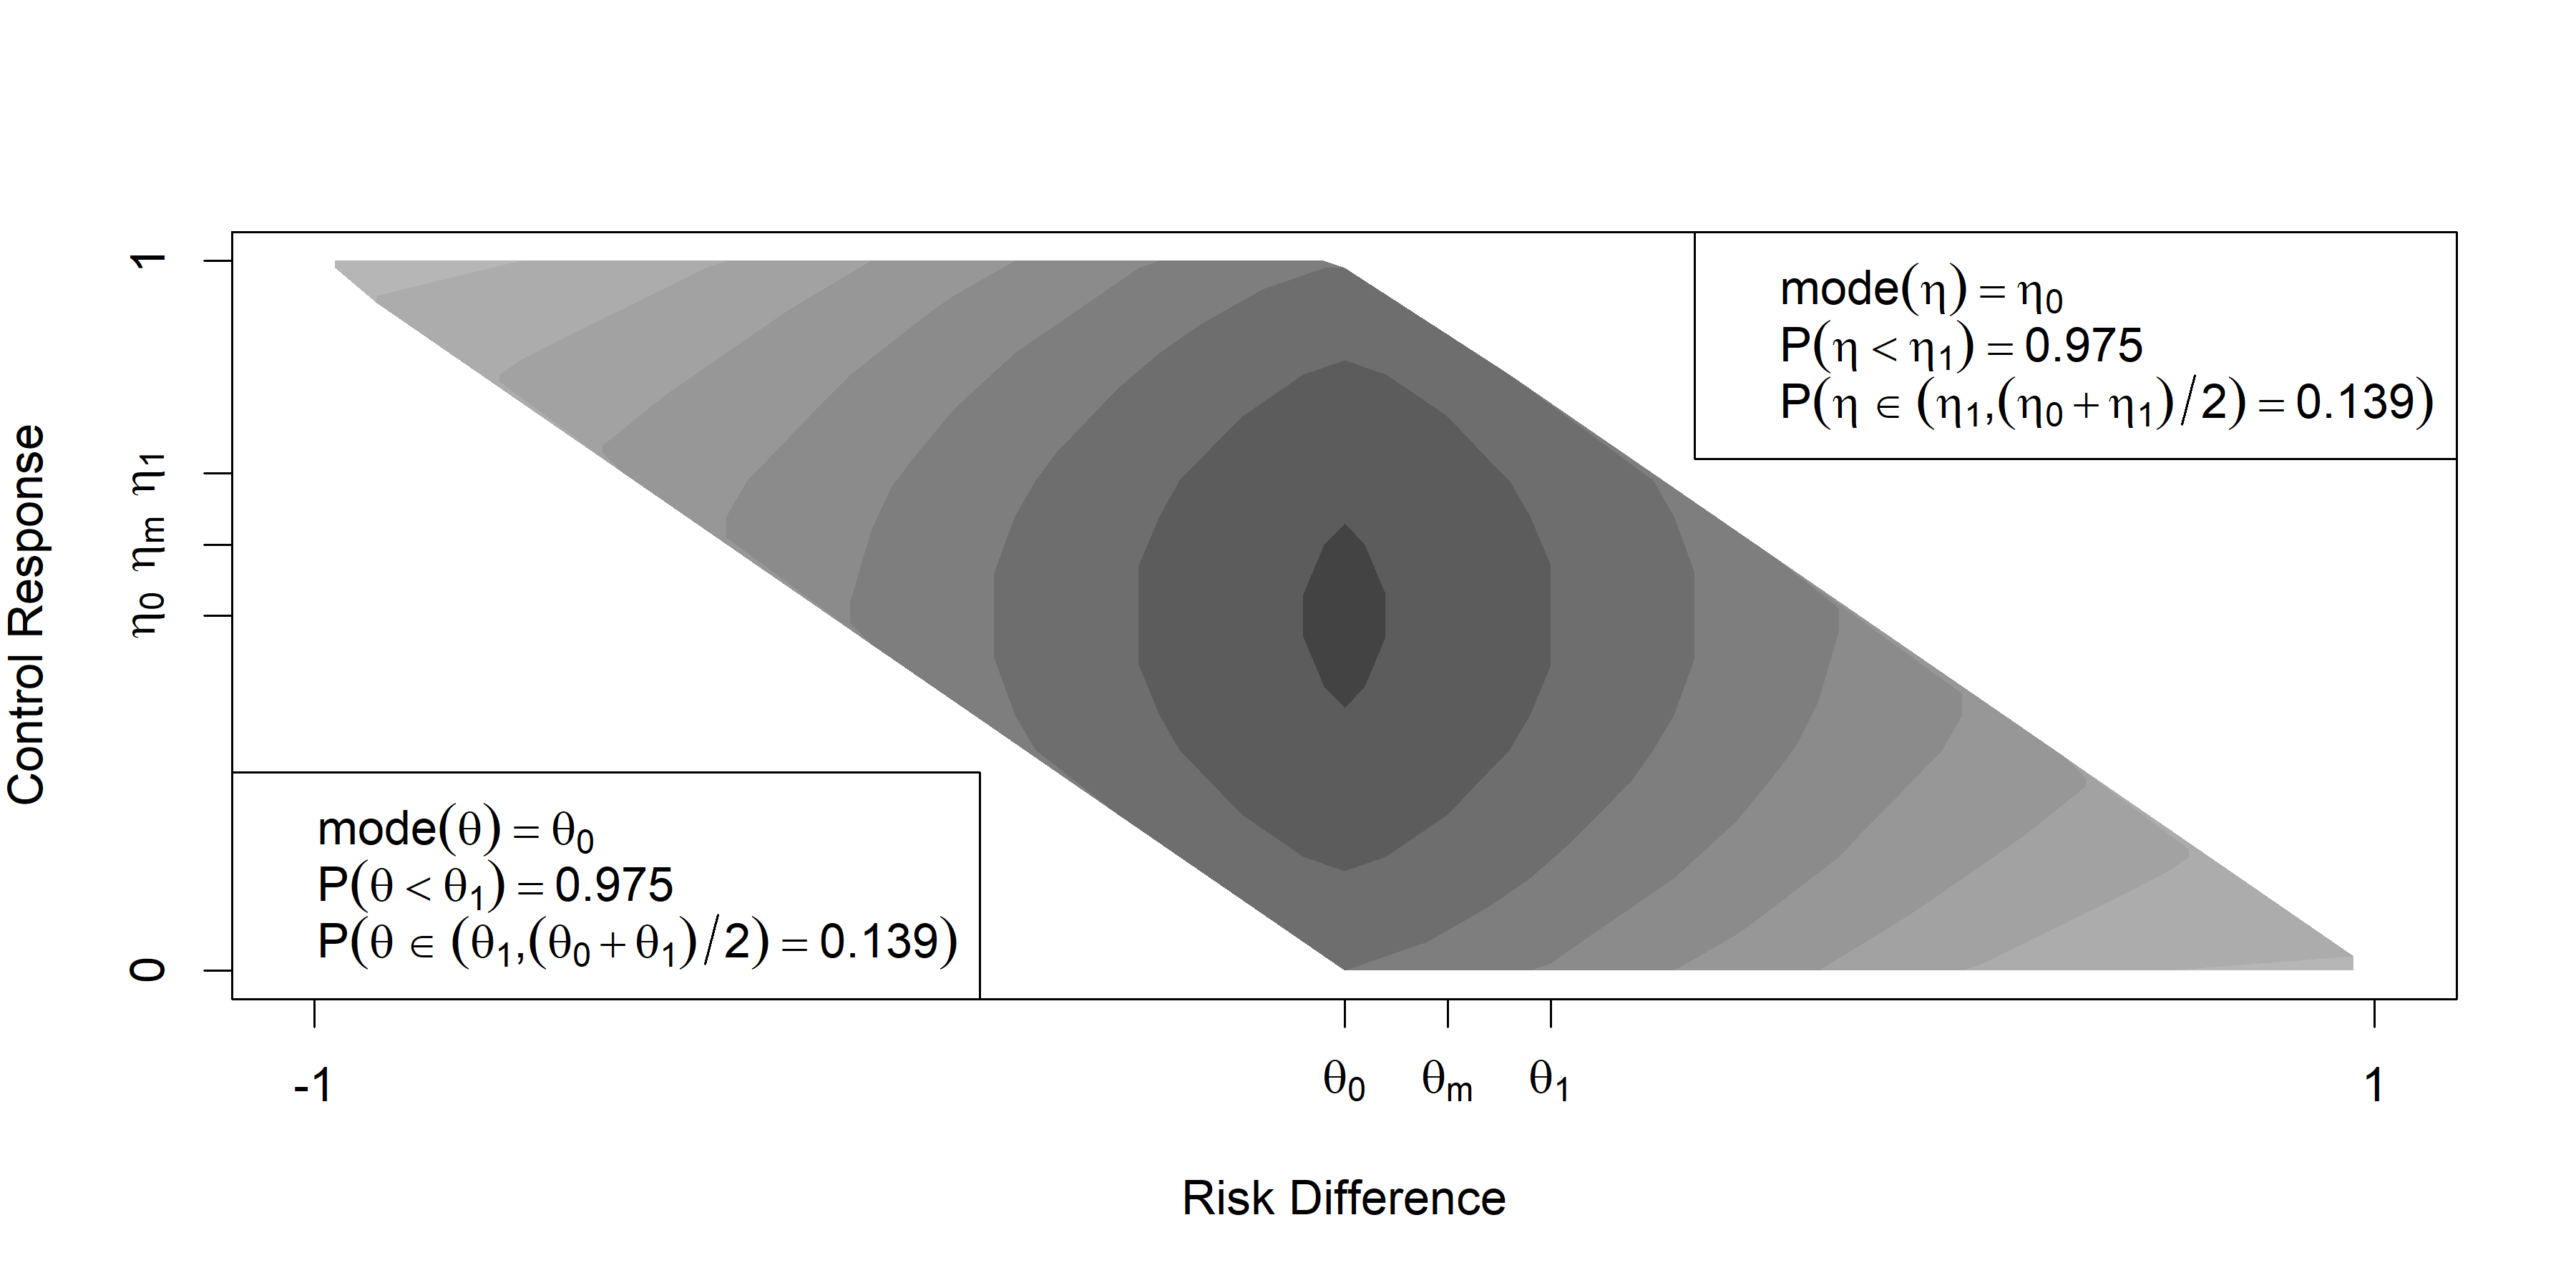
\includegraphics[width=6in]{figure5a.png}
%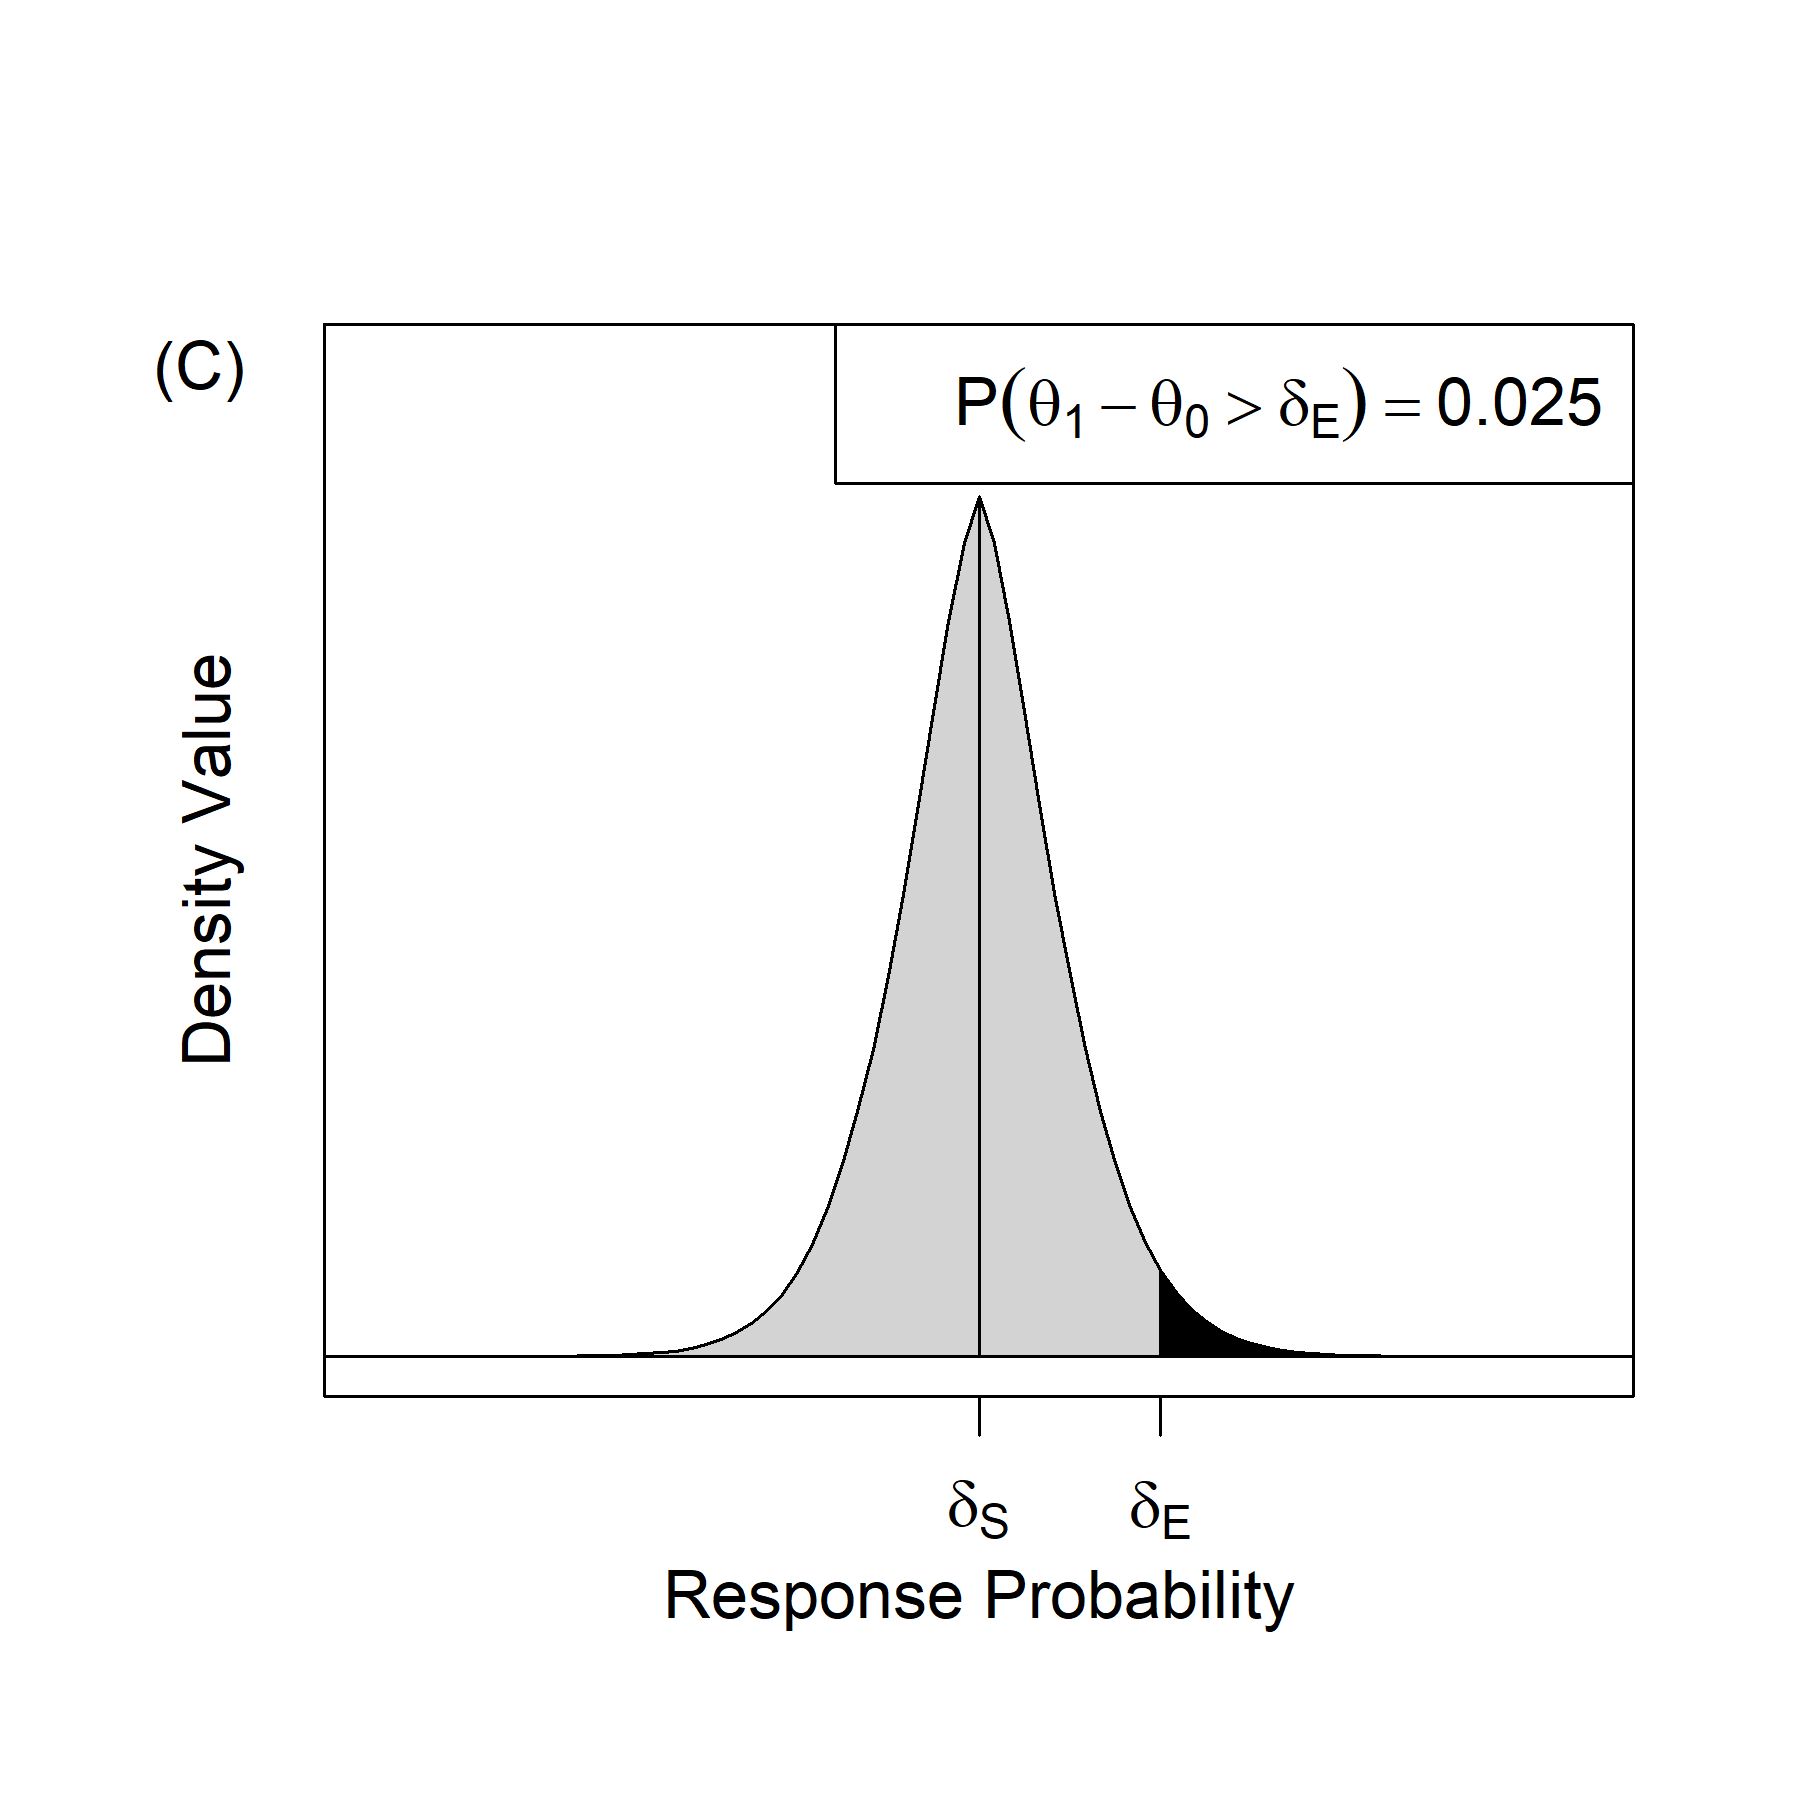
\includegraphics[width=6in]{figure5d.png}
%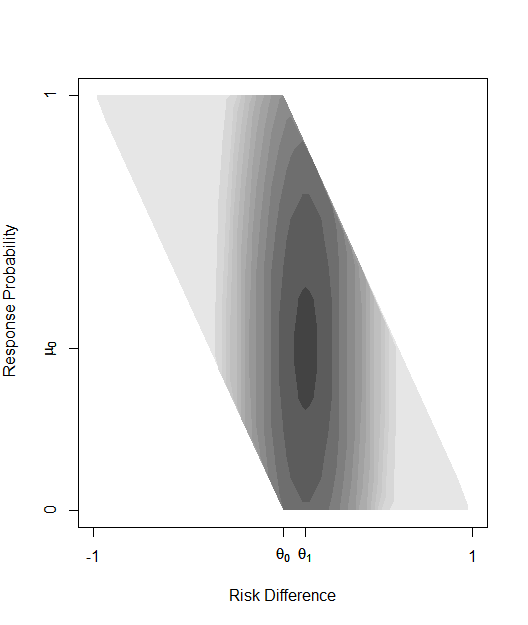
\includegraphics[width=6in]{figure5b.png}
%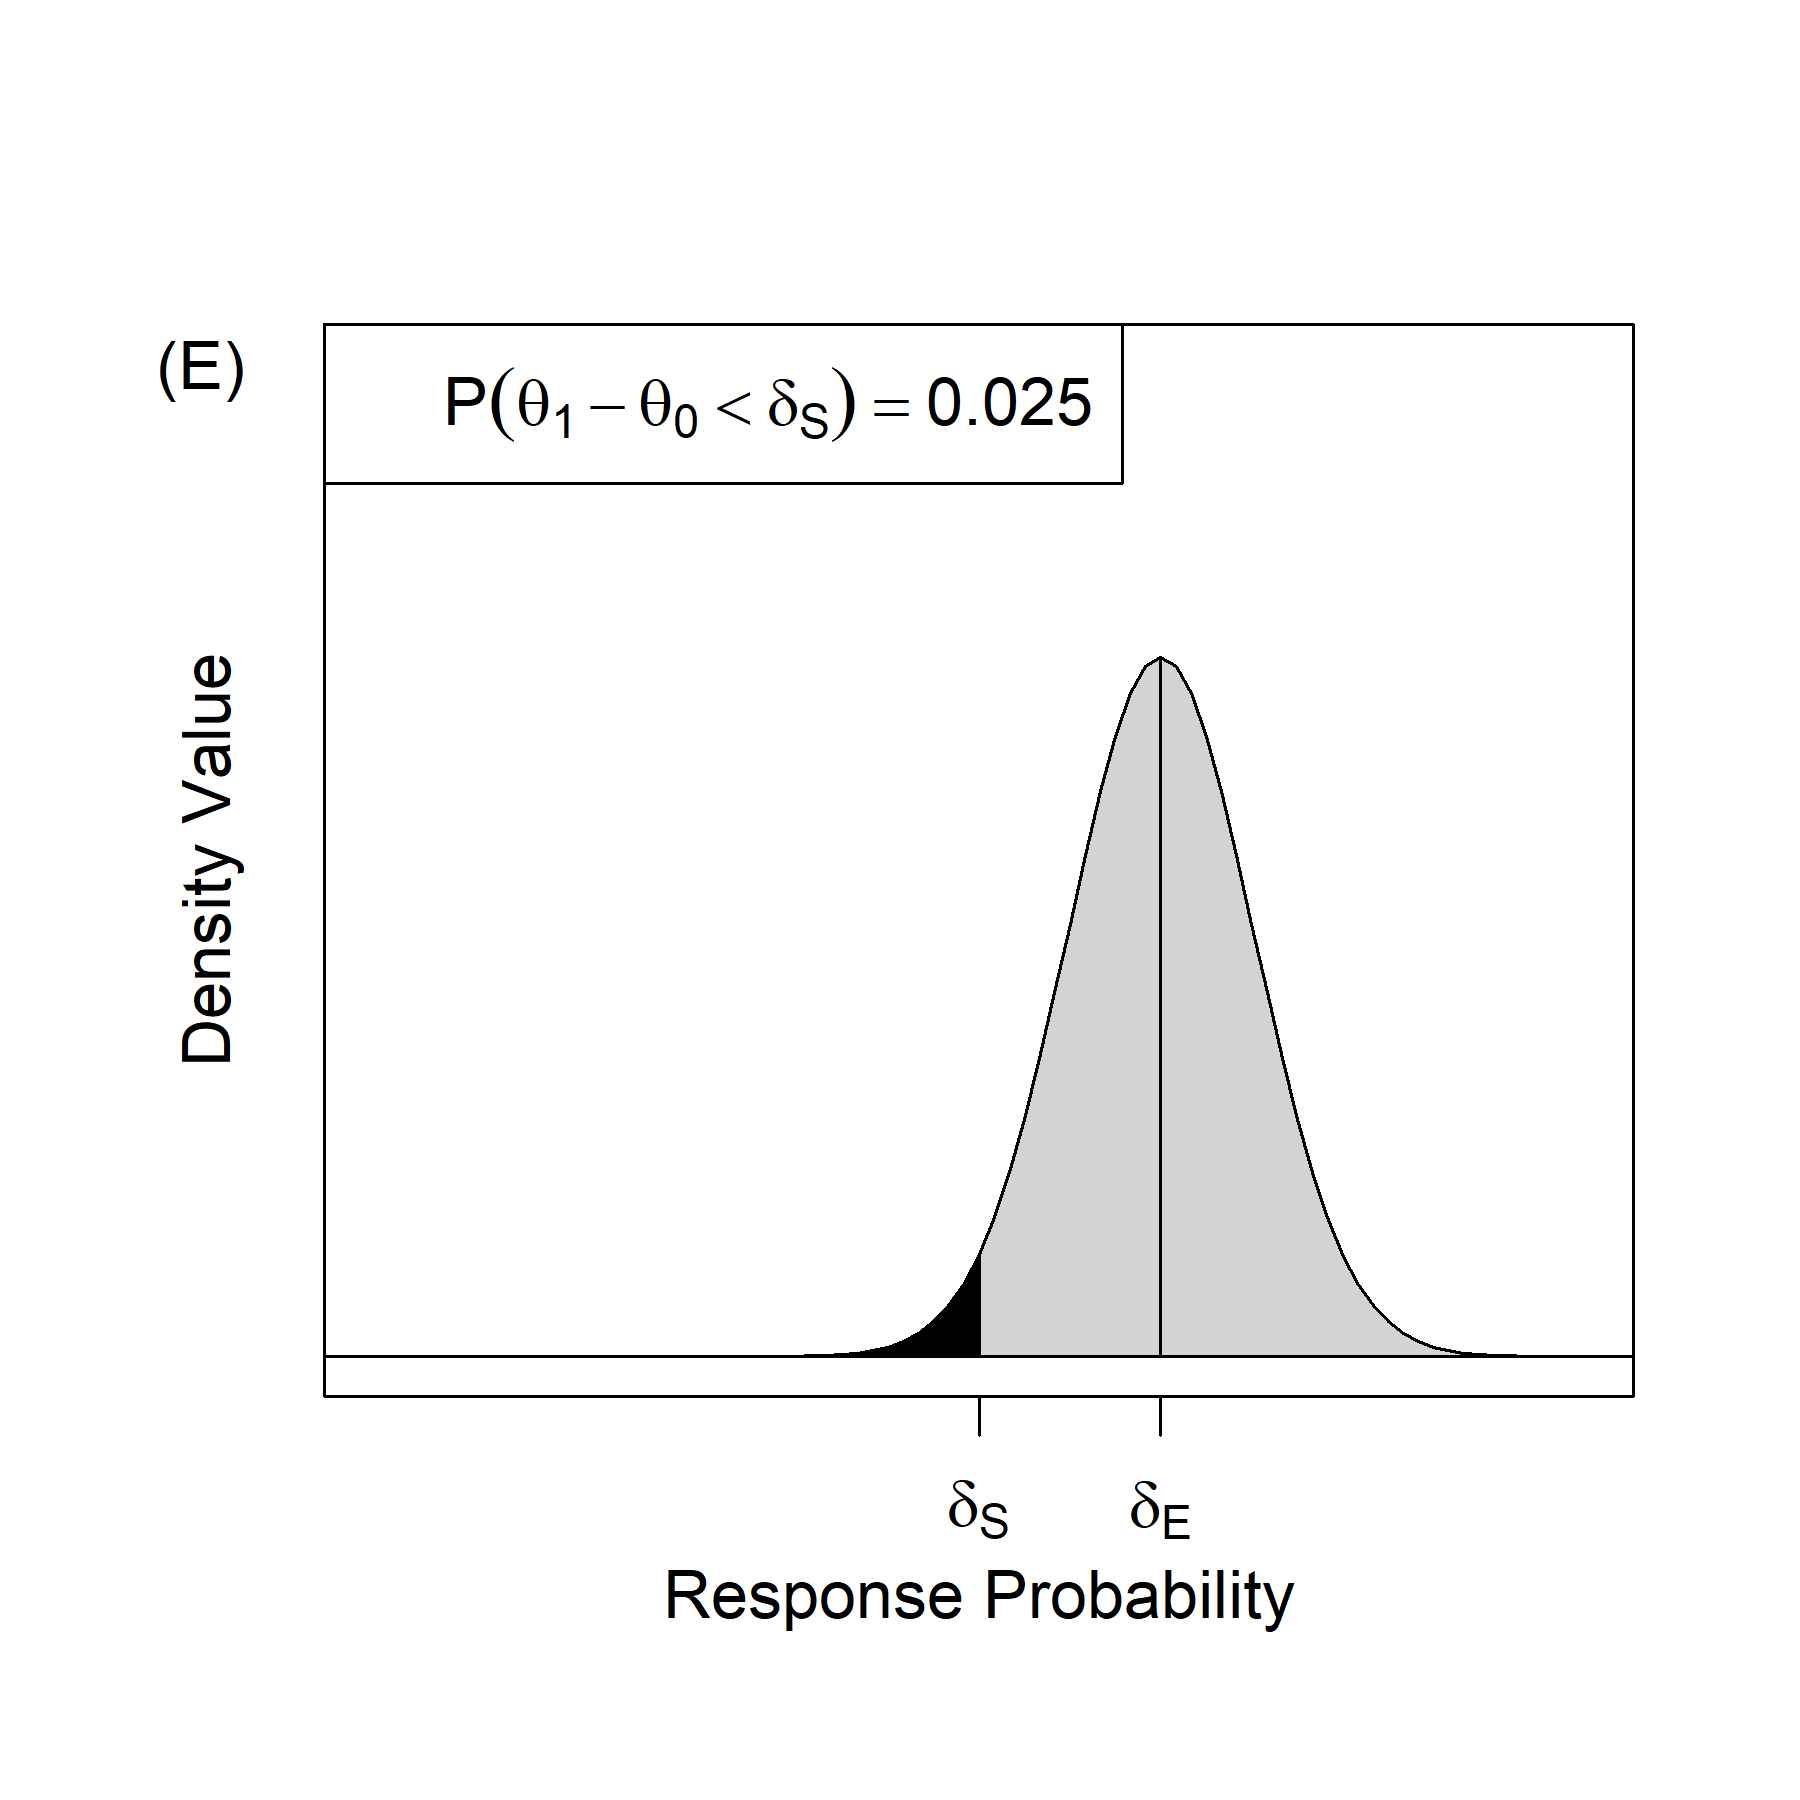
\includegraphics[width=6in]{figure5e.png}
\caption{Joint distribution $\pi(\theta,\eta)=\pi(\theta)\times\pi(\eta|\theta)$, where $\pi(\theta)$ is a default skeptical prior truncated to $[-1,1]$, and $\pi(\eta|\theta)$ is a default skeptical prior truncated to $[\rmn{max}(-\theta,0),\rmn{min}(1,1+\theta)]$.}
\label{fig:figure5}
 \end{center}
\end{figure}

\subsection{Operating Characteristics}
\subsubsection{Expected sample size and trial duration}
Suppose that the trial has interim analyses based on the number of completed outcomes. Let $\bmath{D}(n)$ denote the data after $n$ completed outcomes are ascertained. Let $n_{\text{initial}}$ be the first instance where either the efficacy criteria \eqref{eq:efficacy_criteria} or futility criteria \eqref{eq:futility_criteria} are satisfied and enrollment is henceforth terminated, or $n_{\text{max}}$ if the efficacy criteria or futility criteria are not satisfied at any point. Let $n_{\text{final}}$ be the final sample size which includes patients whose outcomes were in progress at the time of enrollment termination. The expected trial duration is determined based the projected time needed for subject enrollment and outcome ascertainment for a number of subjects equal to the expected sample size.

\subsubsection{Posterior mean and coverage probability}
Any prior of the form \eqref{eq:inference_prior} and the data likelihood $\mathcal{L}(\theta|\mathbf{D})$ are used to evaluate the posterior distribution for $\theta$ denoted $\pi(\theta|\mathbf{D})$. The posterior mean at the final sample size is $E(\pi(\theta|\mathbf{D}(n_{\text{final}}))$. The coverage probability is the probability of the generating value of $\theta$ to be in an equal-tailed $100(1-\alpha)\%$ credible interval, which is the interval $[\theta^{(\alpha/2)},\theta^{(1-\alpha/2)}]$ based on the quantiles of the posterior distribution $\pi(\theta|\mathbf{D}(n_{\text{final}}))$.

\subsubsection{Probability of efficacy, futility, and inconclusive findings}
The probability of stopping early for efficacy and futility are the probability that the efficacy criteria \eqref{eq:efficacy_criteria} or futility criteria \eqref{eq:futility_criteria} are satisfied at an interim analysis with data $\mathbf{D}(n_{\text{initial}})$. The final determination of efficacy and futility refer to the corresponding criteria begin satisfied with data $\mathbf{D}(n_{\text{final}})$. To evaluate the frequentist properties of Bayesian designs, type I error and power are based on $\rmn{eff}(\bmath{D}(n_{\text{initial}}))$.  Inconclusive findings refers to situations where neither the efficacy or futility criteria are satisfied.

\subsubsection{Distribution of final posterior probability of efficacy given interim stoppage}\label{sec:evid_decrease}
Given that the efficacy criteria was satisfied as an interim analysis, it is of interest to compare the associated value once subjects in follow-up have completed outcomes.  It is of particular interest when $\rmn{eff}(\bmath{D}(n_{\text{initial}}))>1-\epsilon$ and $\rmn{eff}(\bmath{D}(n_{\text{final}}))\leq1-\epsilon$, that is, the threshold for substantial evidence is satisfied for an interim analysis but is no longer satisfied once outcomes from patients in progress are ascertained. It is of interest to determine the probability of such an occurrence and the difference between the efficacy criteria evaluated at the different time points.

%\subsection{Design Considerations}
%\begin{enumerate}
%\item DC \#1
%\item DC \#2
%\item DC \#3
%\item DC \#4
%\item DC \#5
%\end{enumerate}

\subsection{Computation}
The efficacy criteria \eqref{eq:efficacy_criteria} and futility criteria \eqref{eq:futility_criteria}, as well as any quantity involving the posterior distribution of $\theta$ requires evaluating integrals of the dimension of $\theta$ (or the dimension of $(\theta,\eta)$ in the case of nuisance parameters). In the examples in Section \ref{sec:examples}, these quantities are $1-$ and $2-$dimensional integrals which are evaluated using numerical integration in R \citep{R2017}, in particular using the pracma package \citep{Borchers2019}.

\section{Examples}\label{sec:examples}

\subsection{Single-Arm Proof-of-Activity Trial with Binary Endpoint}\label{sec:example1}
\subsubsection{Motivating Example}
Consider the T72 pediatric trial ``A Study of the Safety and Efficacy of Infliximab (REMICADE) in Pediatric Patients With Moderately to Severely Active Ulcerative Colitis" (NCT00336492) ~\citep{Hyams2012}. Infliximab was given to all patients at the 5mg/kg dose at weeks 0, 2, and 6, and the primary endpoint was response at week 8. Response was measured by improvement in disease severity scores. The trial was conducted between August 2006 and June 2010. Patients were enrolled over approximately 33.5 months (approximately 1 patient enrolled per 17 days). The sample size of 60 patients was chosen to ensure 12\% precision in estimating the true
response proportion with 95\% confidence interval, assuming a response rate of 0.67 as was observed among adults from the ACT 1 and ACT 2 trials \citep{Rutgeerts2005} at the same 5mg/kg dose (N = 242). A 95\% confidence interval that excluded 0.40 was determined to be a clinically significant result. At week 8, clinical response was observed in 44 out of 60 (73.3\%) patients.


\subsubsection{Model Formulation \& Prior Elicitation}\label{sec:example1model} We use this trial as a template to demonstrate our framework for sequential monitoring. The data $\bmath{D}$ are assumed to be independent Bernoulli random variables with common response probability $\theta$. 
%
This trial has a superiority hypothesis with null response value is $\theta_0=0.4$. For purposes of monitoring, a highly efficacious response probability is $\theta_1=0.67$ and an intermediate response value is $\theta_m=0.535$. 
%
The monitoring priors used are a concentrated skeptical prior and a default enthusiastic prior.
%The skeptical prior is $\pi_S(\theta)\sim\mathcal{GN}_{p=0.975,\Theta=[0,1]}(\tilde{\mu}=\theta_0,q=\theta_1,\gamma=0.75)$. The scaling factor $\gamma<1$ was chosen to concentrate the distribution around the modal value to provide additional Type 1 error control. 
%
%The enthusiastic prior is $\pi_E(\theta)\sim\mathcal{GN}_{p=0.025,\Theta=[0,1]}(\tilde{\mu}=\theta_1,q=\theta_0,\gamma=1)$. The scaling factor $\gamma=1$ was chosen as a default value corresponding to the truncated normal distribution.
%
A comparison of the various combinations of the monitoring priors is provided in Appendix \ref{sec:priorRobustness}.

An inference prior is defined as the mixture \eqref{eq:inference_prior} with $\omega=0.5$.
%
The maximum sample size was increased from $60$ to increase the probability of stopping the trial early due to efficacy at response proportion values between the null $\theta_0=0.4$ and the adult data $\theta_1=0.67$. The sample size of $n_{\text{max}}=112$ based on a frequentist design to have $80\%$ power to conclude efficacy with the skeptical monitoring prior at a true response proportion of $\theta_m=0.535$. This increased power provides a better setting to demonstrate how the flattening or concentration of the skeptical monitoring prior impacts the operating characteristics. Consider an interim analysis occurring after every 2 patients complete follow-up.

\subsubsection{Preposterior Analysis of Operating Characteristics}\label{sec:ex1.1}
The following are generated from $10,000$ simulations for the trial described in Section \ref{sec:example1model}. Figure \ref{fig:ex1.1}(a) shows the operating characters of this particular trial design.
%

When the true response probability is $\theta_0=0.4$, there is a $3.9\%$ probability of stopping the trial early for efficacy. This is higher than the nominal rate of $0.025$ due to the frequent data monitoring after every 2 completed outcomes (see also Section \ref{sec:ex1t1e}). When the true response probability is $\theta_m=0.535$, there is a $80.8\%$ probability of stopping the trial early for efficacy, which is comparable to a frequentist design with one analysis at the maximum sample size of $112$. The probability of stopping the trial for efficacy approaches $100\%$ for response values at $\theta_1=0.67$, and accordingly the expected number of 35.8 patients is the lowest.
%
The probability of stopping early for futility is the highest at the null response rate of $\theta_0=0.4$, and then decreases as data is shown to be compatible with the alternative hypothesis that $\theta>\theta_0$. The impact of futility monitoring at $\theta_0=0.4$ is an expected sample size of 79.2.
%
The probability of inconclusive findings is the greatest at $\theta=0.4675$, where there is often modest evidence that $\theta>\theta_0$ but not enough to satisfy the efficacy criteria at by the chosen maximum sample size. Accordingly, the expected sample size of 91.4 patients is the highest at this value.

For all the generating true response probabilities considered, the expected sample size is much less than the maximum of 112. The trial reaches the maximum sample size it at most 42\% of cases at the response rate of $\theta=0.4675$. Therefore this design benefits from reaching conclusions of efficacy at acceptable levels while reaching them sooner than the maximum sample size.

A mixture prior that equally weighs the skeptical and enthusiastic monitoring priors was used to derive the posterior mean and coverage probabilities. For the generating values of $\theta$ considered, the posterior mean shows bias towards the alternative hypothesis. This is because the inference prior is still informative towards to alternative hypothesis. The coverage probability of an equal-tailed $95\%$ credible interval is shown to cover the true generating value of $\theta$ with more than $95\%$ probability when $\theta$ is near $\theta_0$ or $\theta_1$, and less than $95\%$ of the time when $\theta$ is an intermediate value (e.g. final coverage probability of $93.1\%$ when $\theta=0.535$. This is because the mixture prior places high prior probability near $\theta_0$ and $\theta_1$ and less prior probability at intermediate values.

Figure \ref{fig:ex1.1}(b) addresses the ``evidence decrease" described in Section \ref{sec:evid_decrease}. The probability of these cases occurring is reflected by the percent agreement between interim and final results. For example, in the situations where the trial is stopped early for efficacy at the generating value of $\theta_0=0.4$, the final efficacy criteria is satisfied $48.2\%$ of the time. This means that the outcomes in progress are likely to show evidence towards the null enough to contradict the conclusion of efficacy. When the trial is stopped early for efficacy and the generating value of $\theta_1=0.67$, the final efficacy criteria is satisfied in $92.0\%$ of cases. The distribution of the efficacy criteria given the final data for these cases are shown. This shows that even in the cases where there is evidence decrease, the final efficacy criteria is still similar to the $1-\epsilon=0.975$ threshold. For example, when the generating value of $\theta_1=0.67$, and in the $8\%$ of situations where there is evidence decrease, over $90\%$ of these cases have a final efficacy criteria of over $0.93$.
%

\begin{figure}\begin{center}

    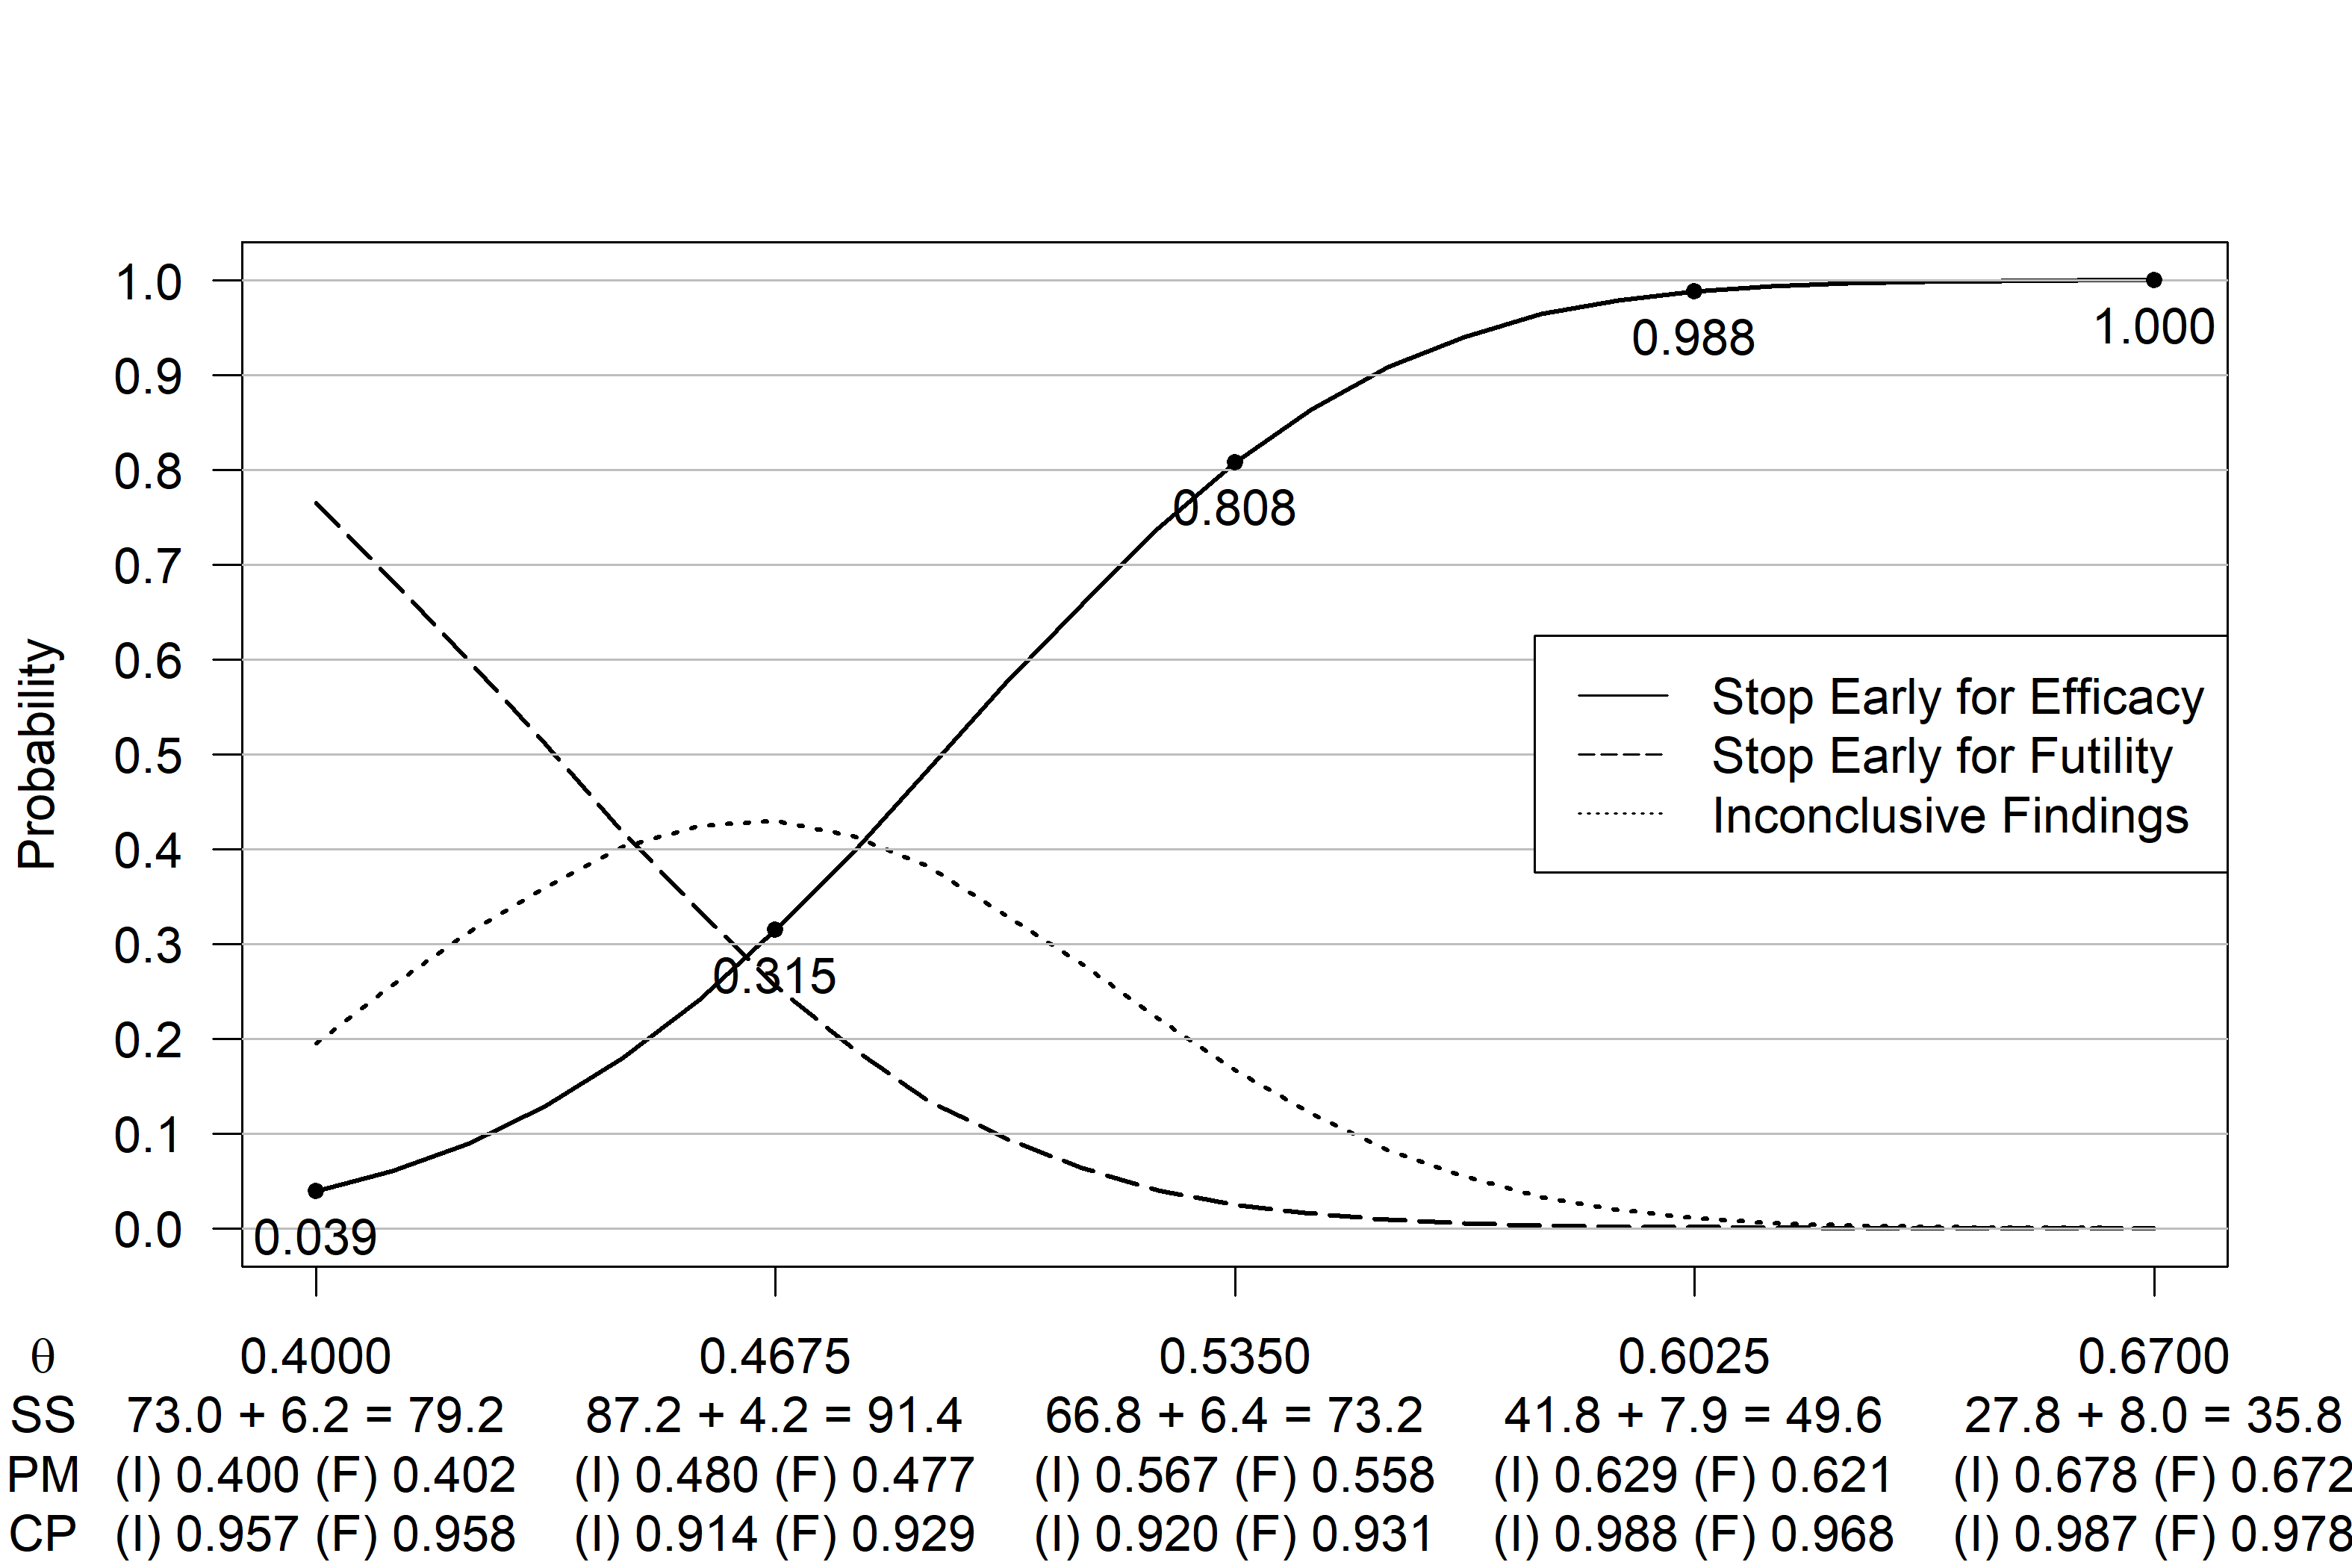
\includegraphics[width=6in]{figure3a.png}
    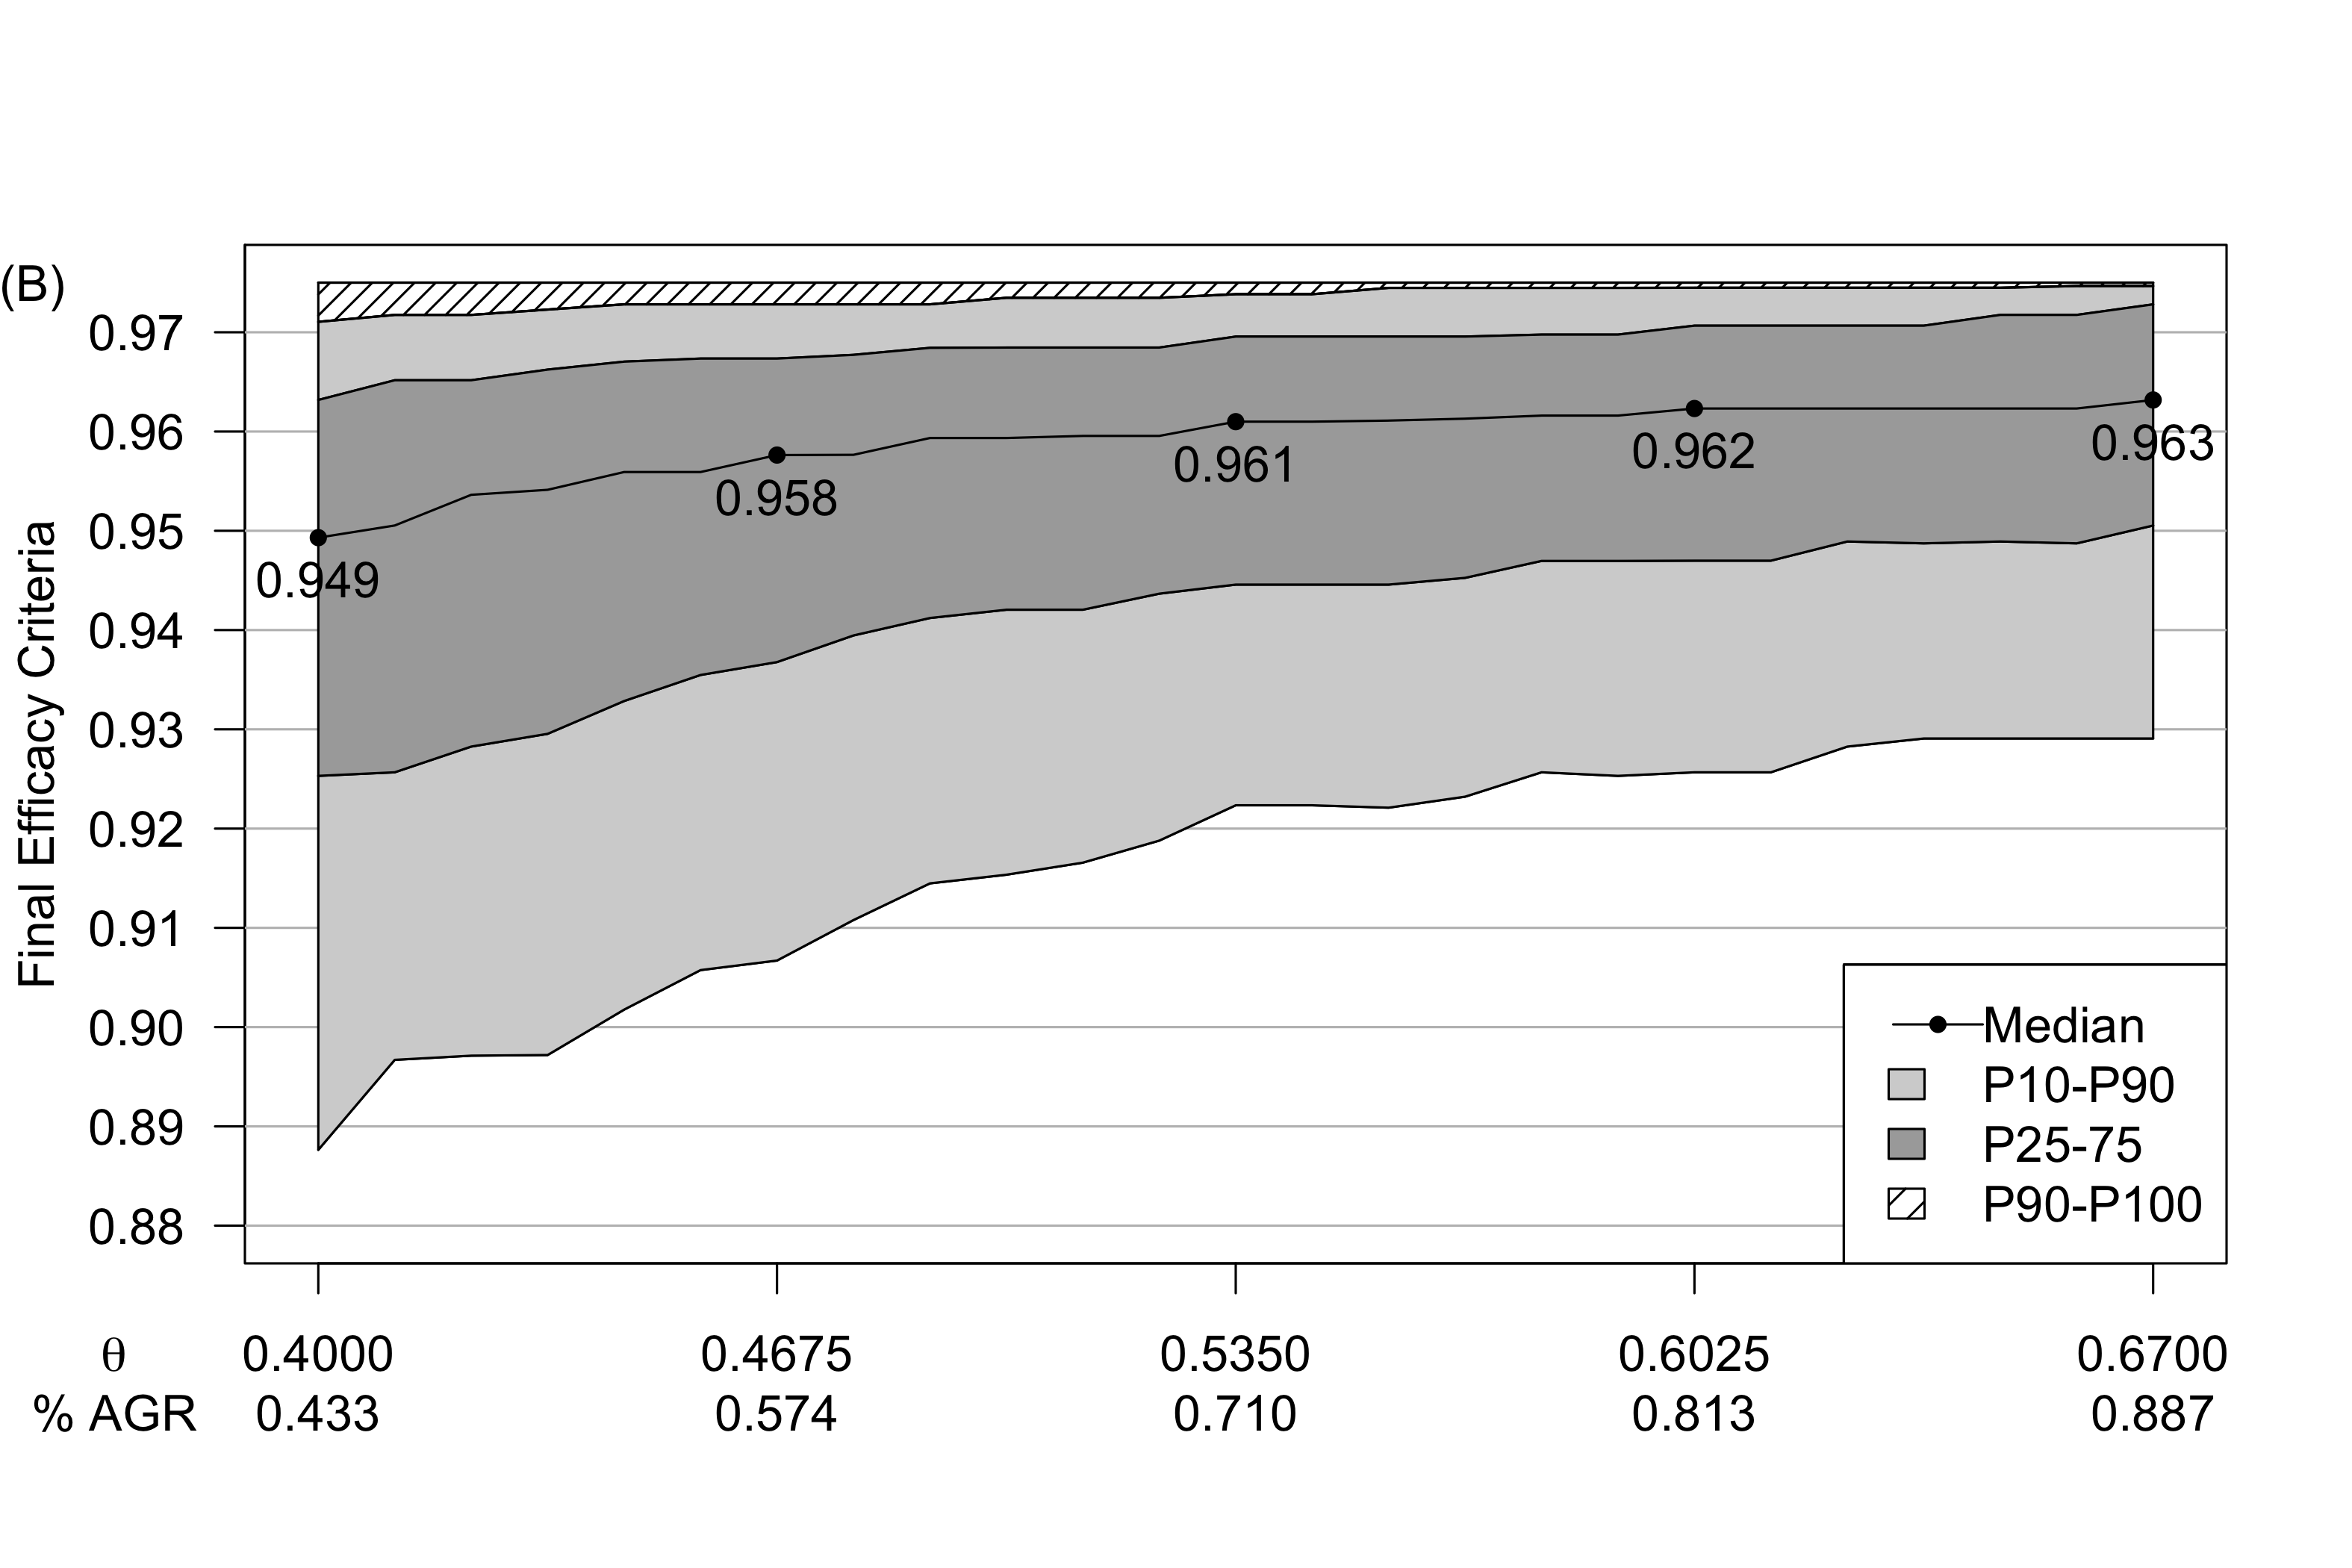
\includegraphics[width=6in]{figure3b.png}
    \caption{A, Sequential design properties. (SS; sample size, PM; posterior mean, CP; coverage probability, (I); interim analysis, (F); final analysis). B, Distribution of final posterior probability given interim stoppage and evidence decrease ($\%$ AGR; Percent of agreement between final and interim posterior probabilities relative to $1-\epsilon$ threshold)}
	\label{fig:ex1.1}

\end{center}
\end{figure}
\subsubsection{Type 1 Error Rate by the Frequency of Data Monitoring}\label{sec:ex1t1e}
Figure \ref{fig:ex1t1e} shows the probability of the efficacy criteria being satisfied at an interim and final analysis when $\theta=\theta_0$. 
%
The monitoring frequency is 1 when an interim analysis is made after every completed outcome (i.e. fully sequential), and is 112 (the maximum sample size) if the only analysis is done at the maximum sample size. When there is only a single analysis completed at the maximum sample size, the probability of determining efficacy is only $0.8\%$. This is because the determination of efficacy is made with an informative skeptical prior. If the determination of efficacy was made with a non-informative prior, then the probability of the efficacy criteria being satisfied with a single analysis completed at the maximum sample size would be $2.5\%$. For more frequent data monitoring, the probability of concluding efficacy is increased from $0.8\%$ to levels even higher than the nominal level of $2.5\%$. This is to be expected; there are more opportunities for a conclusion of efficacy to be made with more frequent interim analyses and it is important that this probability is examined and viewed as an acceptable trade-off for advantages such as the corresponding decrease in expected sample sizes.
\begin{figure}\begin{center}

    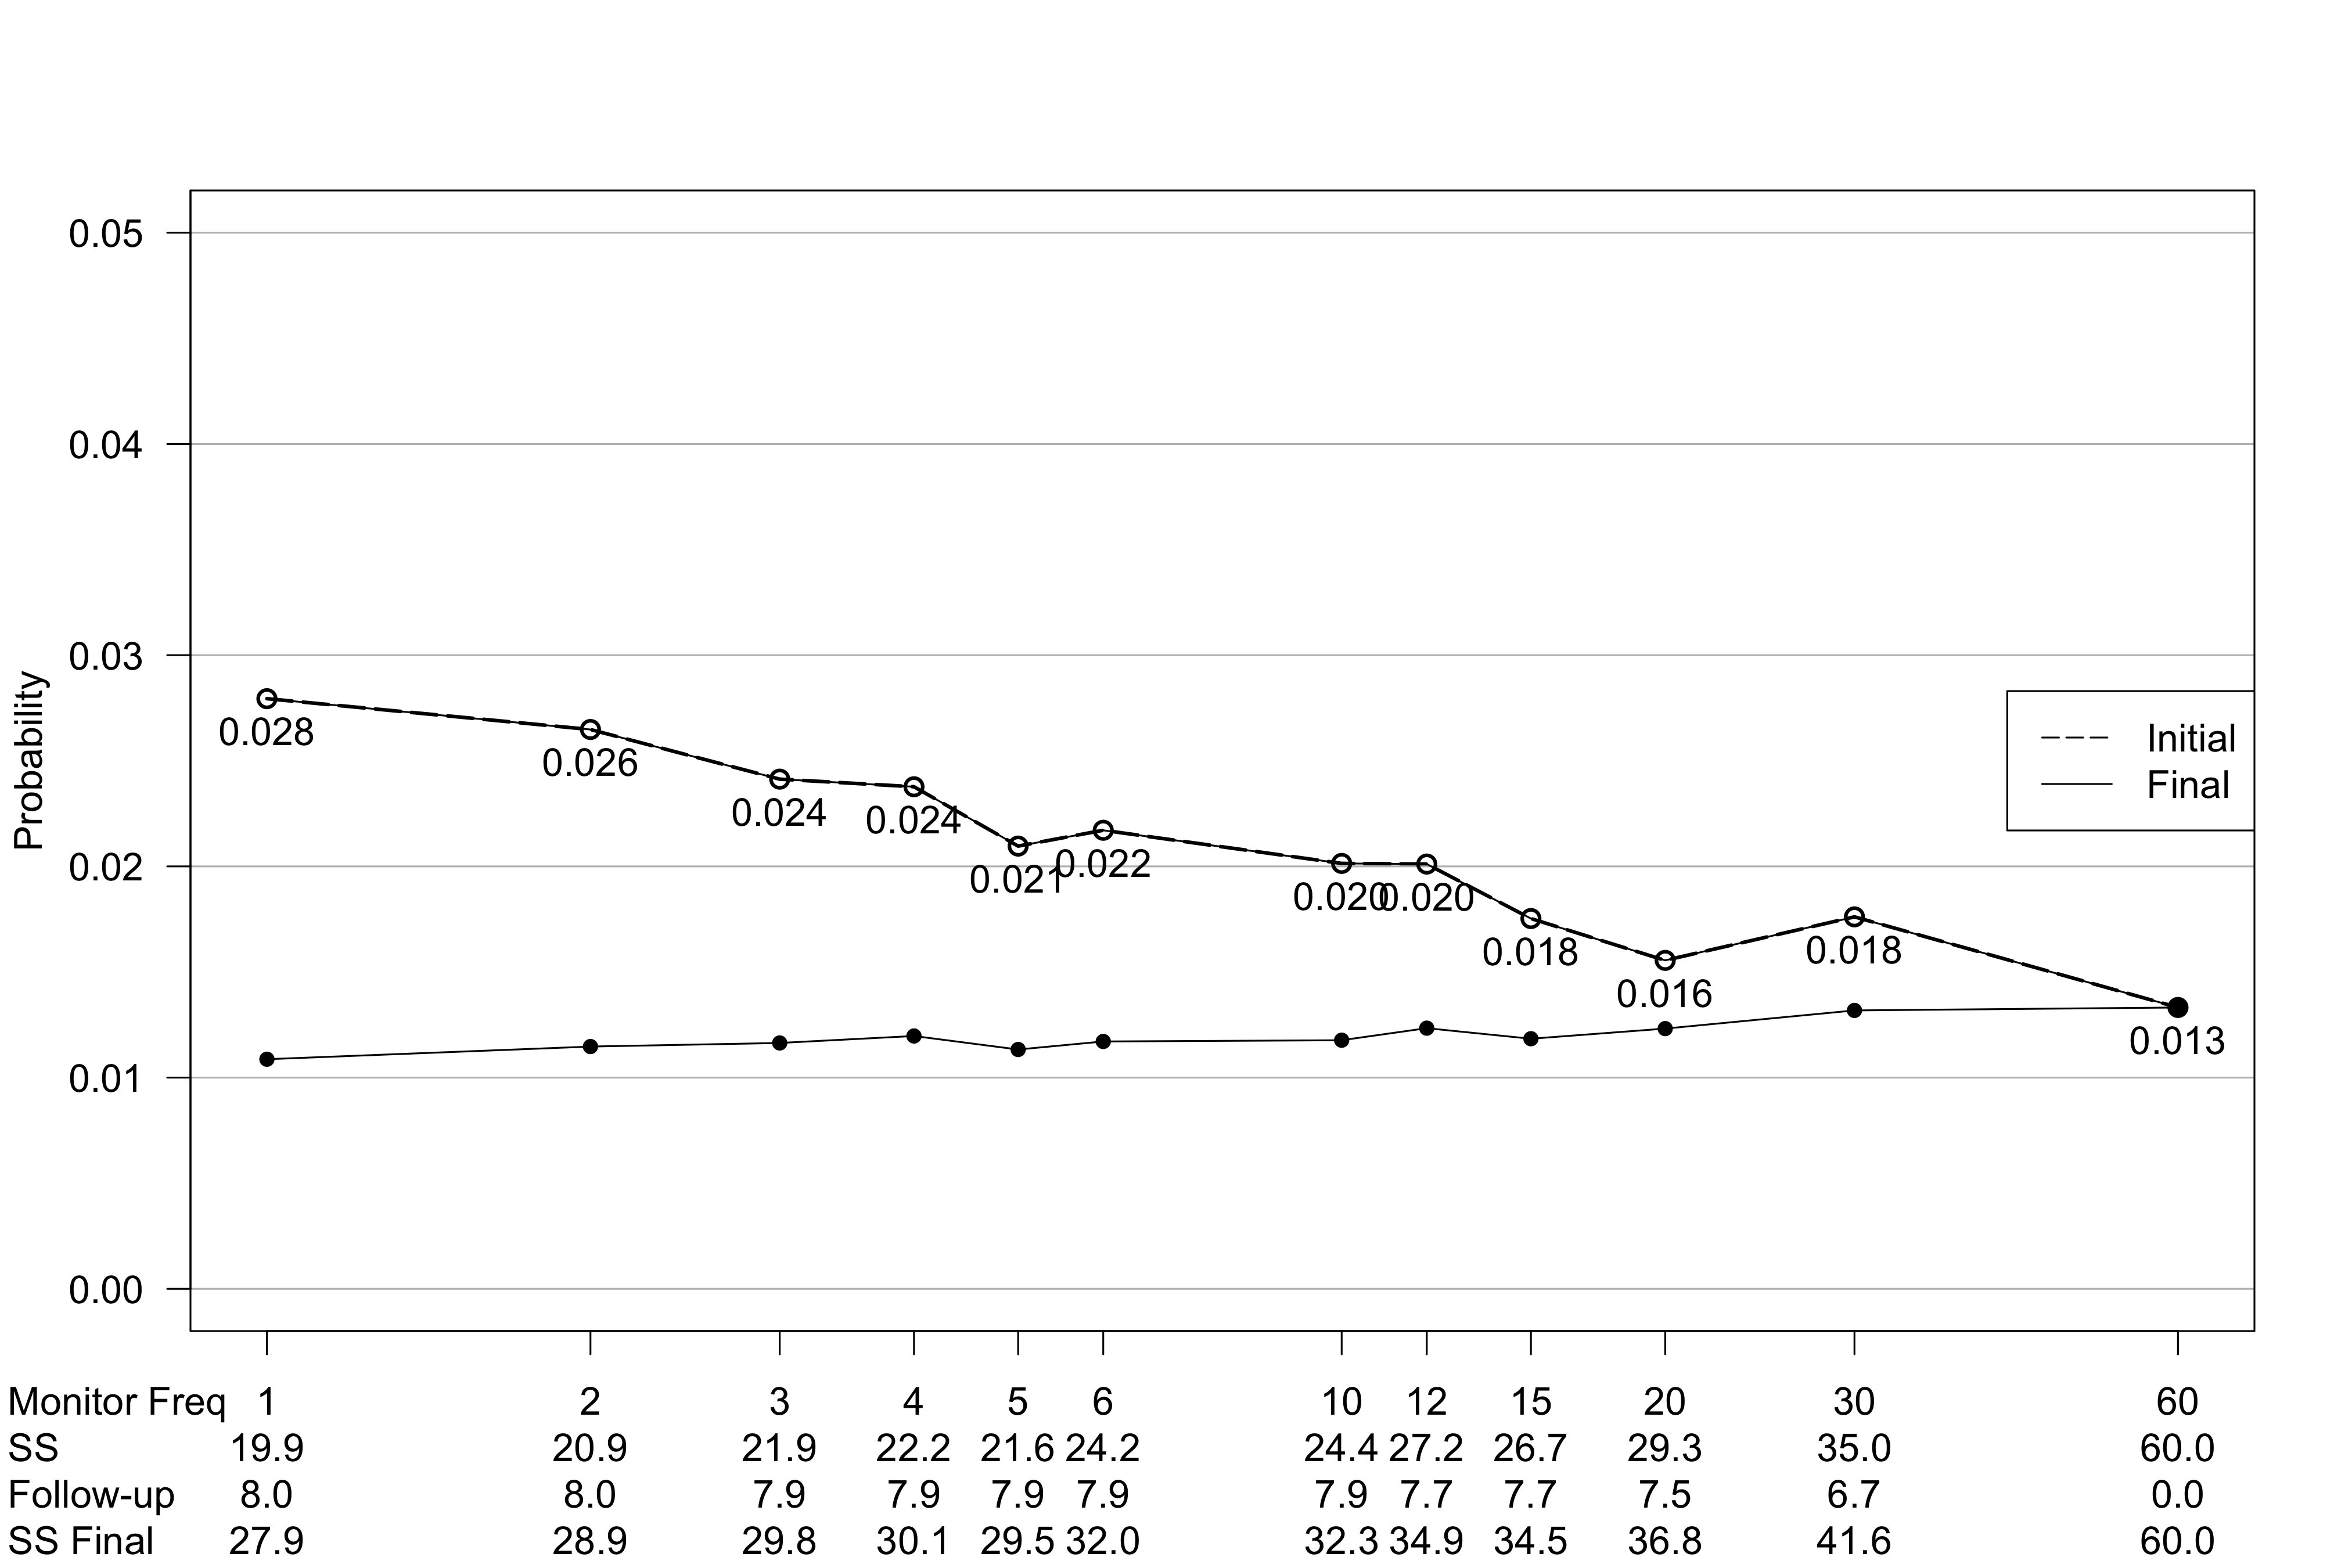
\includegraphics[width=6in]{figure4.png}
    \caption{Probability of efficacy criteria being satisfied when $\theta=\theta_0$. SS; sample size. Monitor Freq; monitoring frequency.}
	\label{fig:ex1t1e}

%  \begin{subfigure}{7in}
%    \centering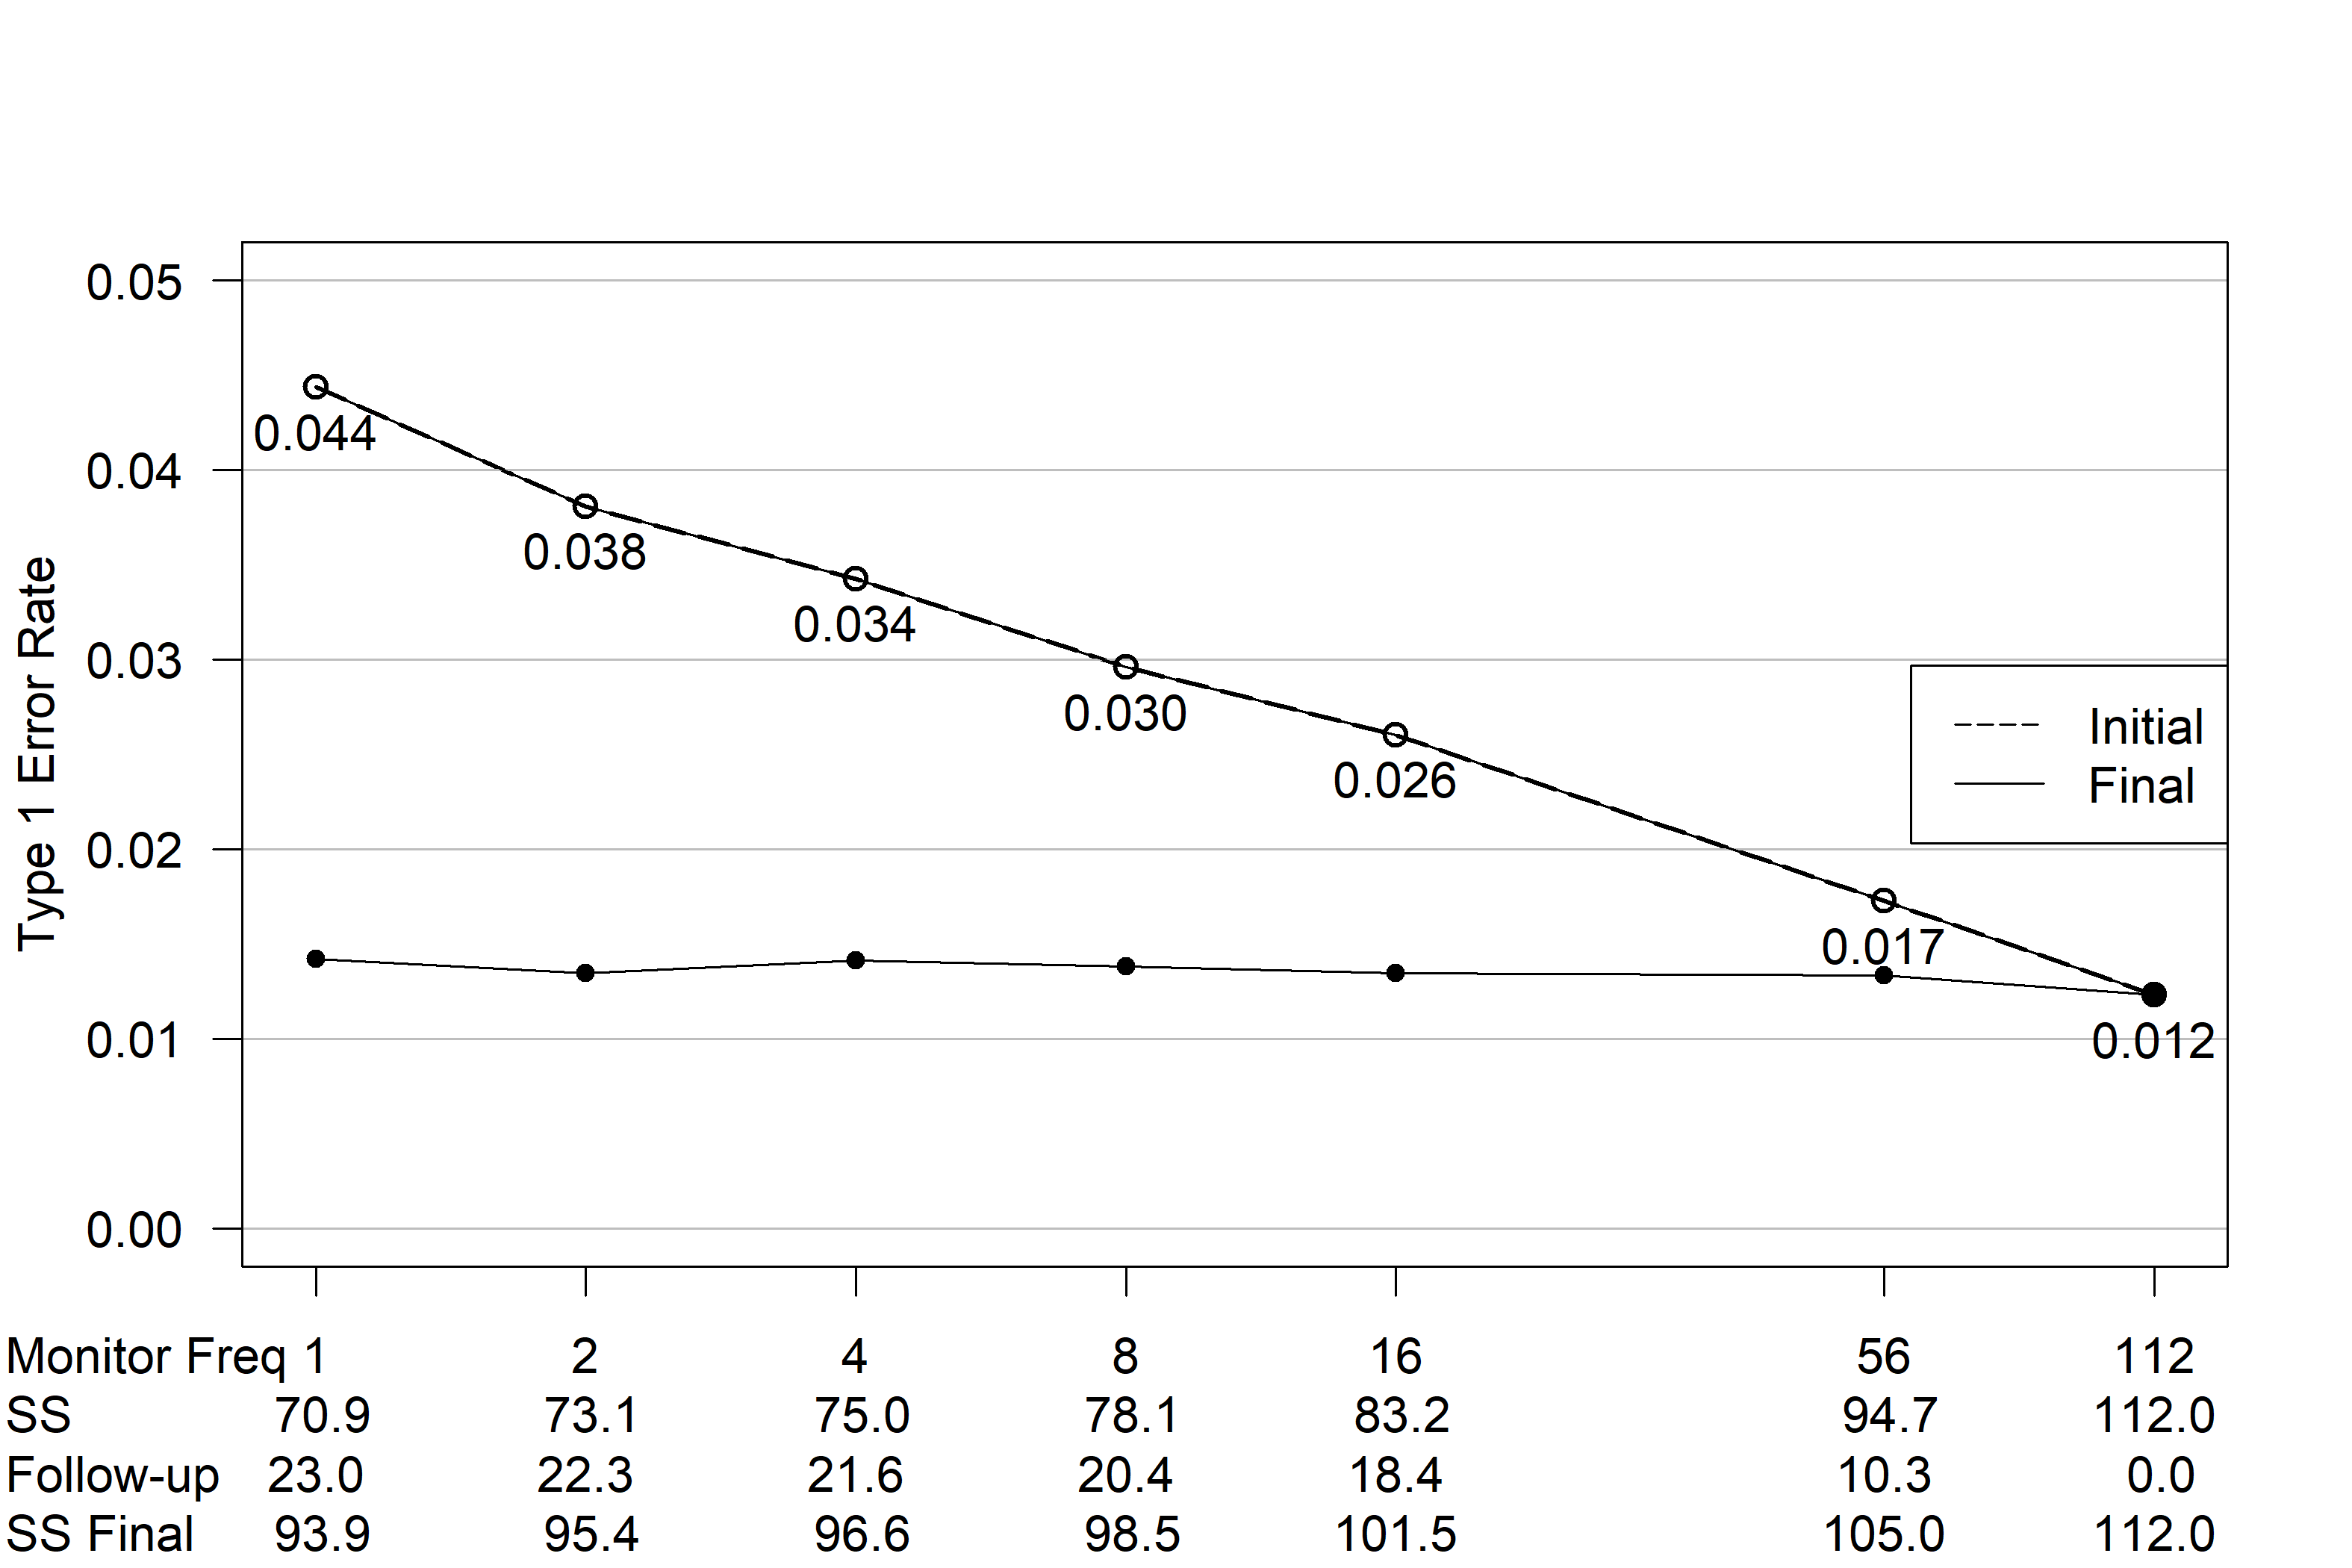
\includegraphics[width=6in]{figureS1.png}
%    \caption{Caption text 2}
%  \end{subfigure}
 
\end{center}
\end{figure}
%\item The two sides of the discussion: first is what happens during the trial regarding sequential monitoring, such as \% of time stopping early vs. trial done to completion and expected sample size. Second is the final determination of efficacy or futility and how that relates to Type 1 Error and power. 
%\item  Remember the best case for sequential monitoring is slow enrollment relative to outcome ascertainment. Slow enrollment means there is a benefit to ending trial early and reach a conclusion faster. Outcome ascertainment needs to be somewhat fast to ensure a good \# of outcomes are generated.

\subsection{Parallel Two-Group Design with Binary Endpoint}\label{sec:example2}
\subsubsection{Motivating Example}
Consider the trial ``The Pediatric Lupus Trial of Belimumab Plus Background Standard Therapy (PLUTO)" (NCT01649765). Patients were randomized to belimumab 10mg/kg or placebo, and the primary endpoint was response at week 52. A binary response variable was measured by improvement in disease severity scores. The goal was to test for superiority of belimumab to placebo. 
The study start date was September 7, 2012, and the primary completion date was January 24, 2018. Since the follow-up period is 52 weeks the last enrollment is estimated to be a year prior to the primary competition date yielding an average enrollment rate of one enrollment per $17$ days. The study design included enrollment of 100 patients, the first 24 patients randomized in a 5:1 ratio (belimumab:placebo) and the remaining 76 patients would be randomized in a 1:1 allocation ratio. Therefore, 58 patients would be randomized to belimumab and 42 to placebo. The sample size was based on feasibility constraints rather than a power calculation, and the study was terminated after 93 patients enrolled.

The results of this trial were inconclusive with the 93 patients. A post-hoc Bayesian analysis that gave $55\%$ weight to adult data with response rate $0.51$ was sufficient to provide evidence of positive treatment effect \citep{Travis2019}. Our method contrasts such a post-hoc analysis with the prospective use of a monitoring prior for efficacy which gives weight to the adult data.

\subsubsection{Model Formulation \& Prior Elicitation}\label{sec:example2model}
We use this trial as a template to demonstrate our framework, in particular the performance of our response-adaptive monitoring prior \eqref{eq:adaptive_prior}. The adaptive prior is useful in this setting because the trial is underpowered and the prospective use of an informative monitoring prior for efficacy provides a different perspective than a post-hoc analysis with an informative prior. The data $\bmath{D}$ are assumed to be independent Bernoulli random variables with response probability $\eta_0$ for the placebo group and $\eta_1$ for the treatment (IP for investigational product) group. 
%
This trial has a superiority hypothesis of IP to control with null treatment difference value of $\theta_0=0$. For purposes of monitoring, a highly efficacious difference probability is $\theta_1=0.12$ \citep{Travis2019} and an intermediate response value is $\theta_m=0.06$ An estimate for the pediatric response rate is $\eta_0=0.39$, which is $0.12$ less than the adult data response rate.

The skeptical monitoring prior is $\pi_S(\theta,\eta_0)=\pi_S(\theta)\times\pi(\eta_0|\theta)$, where $\pi_S(\theta)$ is a concentrated skeptical prior. The enthusiastic monitoring prior is $\pi_E(\theta,\eta_0)=\pi_E(\theta)\times\pi(\eta_0|\theta)$, where $\pi_E(\theta)$ is a default enthusiastic prior. The probability of concluding efficacy at an interim analysis is made using a mixture prior with dynamic weight of the form \eqref{eq:adaptive_prior}. A 3-part mixture inference prior of the form \eqref{eq:3partmix} will be used to estimate the posterior mean and coverage probabilities for $\theta$. The locally non-informative prior is $\pi_{NI}(\theta,\eta_0)=\pi_{NI}(\theta)\times\pi(\eta_0|\theta)$. For the skeptical, enthusiastic, and locally non-informative priors, $\pi(\eta_0|\theta)$ is a flattened prior with modal value $0.39$ and tail probability condition $P(\eta_0>0.59 | \theta)=0.025$.

%, where $\pi_S(\theta)\sim\mathcal{GN}_{p=0.975,\Theta=[-1,1]}(\tilde{\mu}=\theta_0,q=\theta_1,\gamma=0.75)$. The value $\gamma=0.75$ reflects a concentrated distribution which was chosen to reflect a conservative opinion for added Type 1 error control. The enthusiastic monitoring prior is $\pi_E(\theta,\eta_0)=\pi_E(\theta)\times\pi(\eta_0|\theta)$, where $\pi_E(\theta)\sim\mathcal{GN}_{p=0.025,\Theta=[-1,1]}(\tilde{\mu}=\theta_1,q=\theta_0,\gamma=1)$. The value $\gamma=1$ was chosen as the default value. For both the skeptical and enthusiastic monitoring prior,$\pi(\eta_0|\theta)\sim\mathcal{GN}_{p=0.975,H=[max(-\theta,0),min(1,1+\theta)]}(\tilde{\mu}=0.39,q=0.59,\gamma=1.5)$. The value $\gamma=1.5$ was chosen to reflect a liberal opinion about the distribution of $\eta_0$. In general, it is recommended to use flattened priors for nuisance parameters.

A maximum sample size of $n_{\text{max}}=100$ was chosen based on the trial protocol. A minimum sample size of $n_{min}=70$ was chosen to provide an adequate number of placebo controls to be enrolled given the initial 5:1 allocation to the treatment group.
%
An interim analysis is competed after every 2 patients have completed outcomes beginning at $n_{min}$.

\subsubsection{Preposterior Analysis of Operating Characteristics}\label{sec:ex2operatingcharacteristics} 


Figure \ref{fig:ex2varyomega}(A) shows the operating characteristics of this design using the adaptive weight monitoring prior and the 3-part mixture inference prior. The generating response probability in the placebo group is 0.39, and the generating response probability in the treatment group is based on risk differences $\theta$ in $\{0, 0.06, 0.12, 0.18, 0.24\}$. When $\theta=0$, there is a 0.008 probability of concluding efficacy at an interim analysis. This probability increases to $0.193$ at $\theta_1=0.12$. At the effect size $0.24$ the probability of concluding efficacy increases to $0.711$, and the expected final sample size is 90.3 patients.

Figure \ref{fig:ex2varyomega}(B) shows the probability of stopping early for efficacy using a fixed weight mixture prior of the form \eqref{eq:inference_prior}  for efficacy monitoring with a fixed choice of $\omega$ chosen at the outset to be in the set $\{0.25,0.5,0.75,1\}$, and the associated sample sizes. Note that $\omega=1$ corresponds to the traditional skeptical prior, $\omega=0.5$ gives equal weight to the skeptical and enthusiastic components, and $\omega=0.25$ most of the weight is applied to the enthusiastic component. The adaptive weight mixture behaves similar to using a fixed weight prior that equally weighs the skeptical and enthusiastic prior.




\begin{figure}\begin{center}
      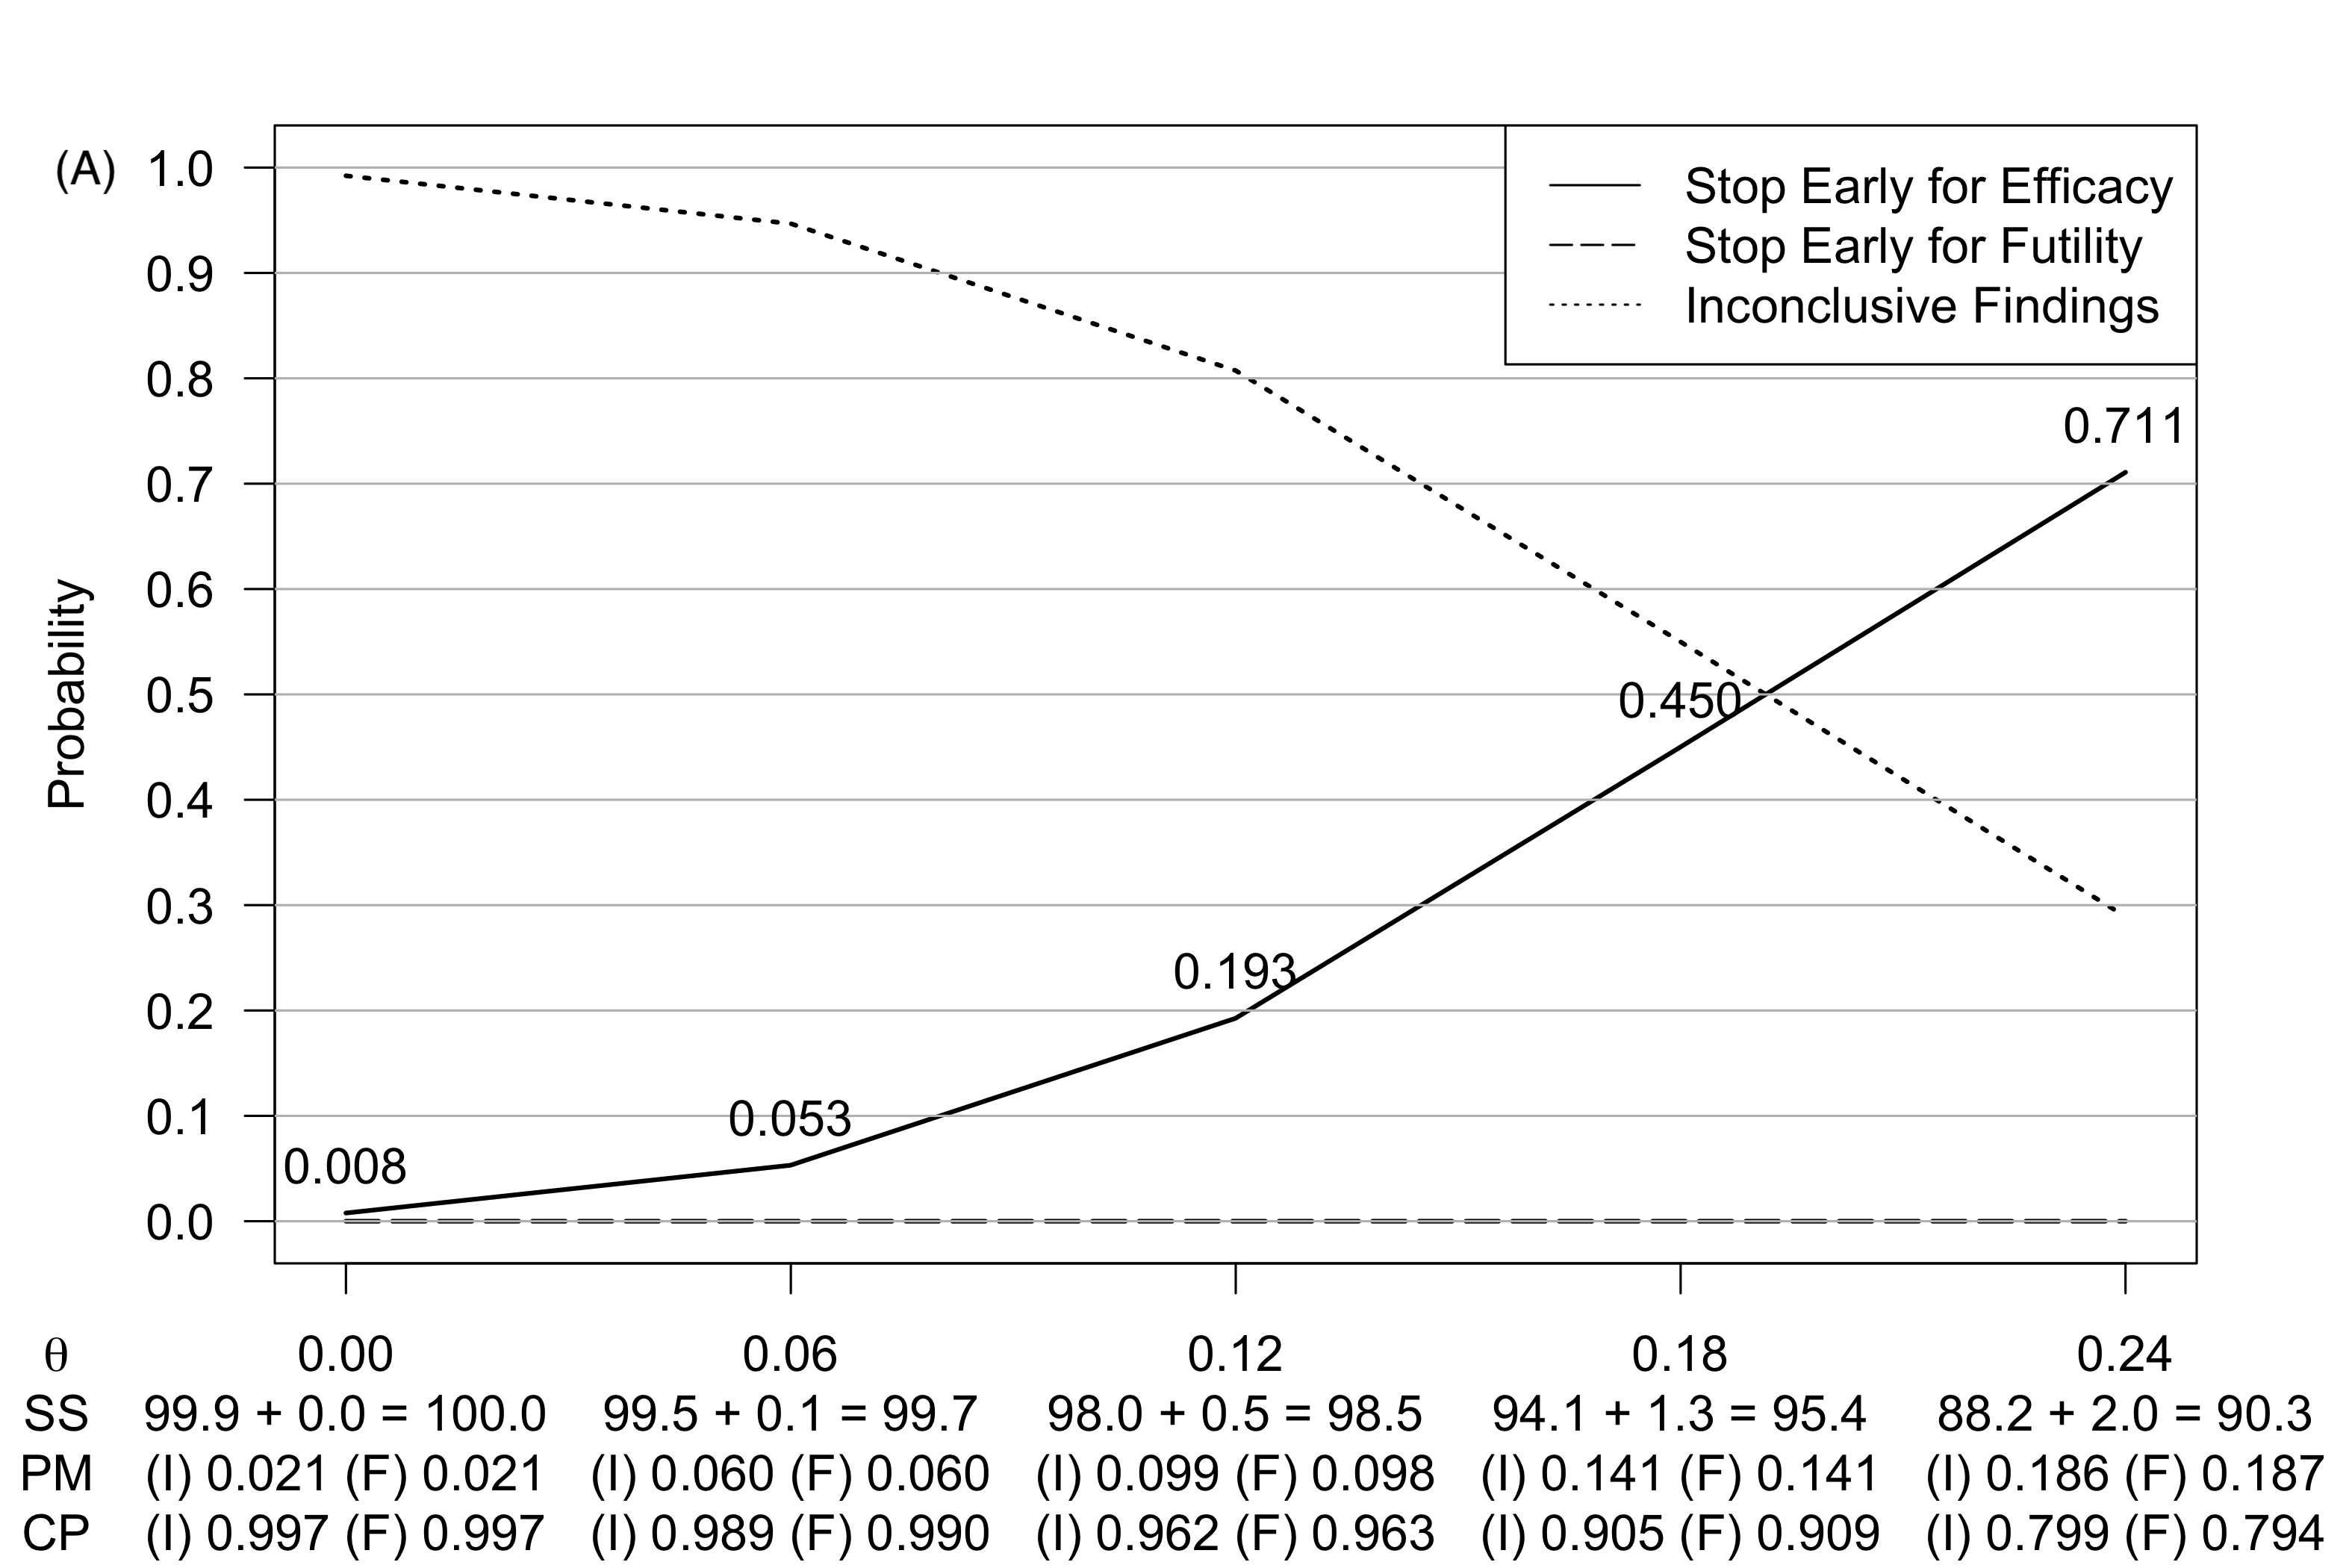
\includegraphics[width=6in]{figure9.png}
   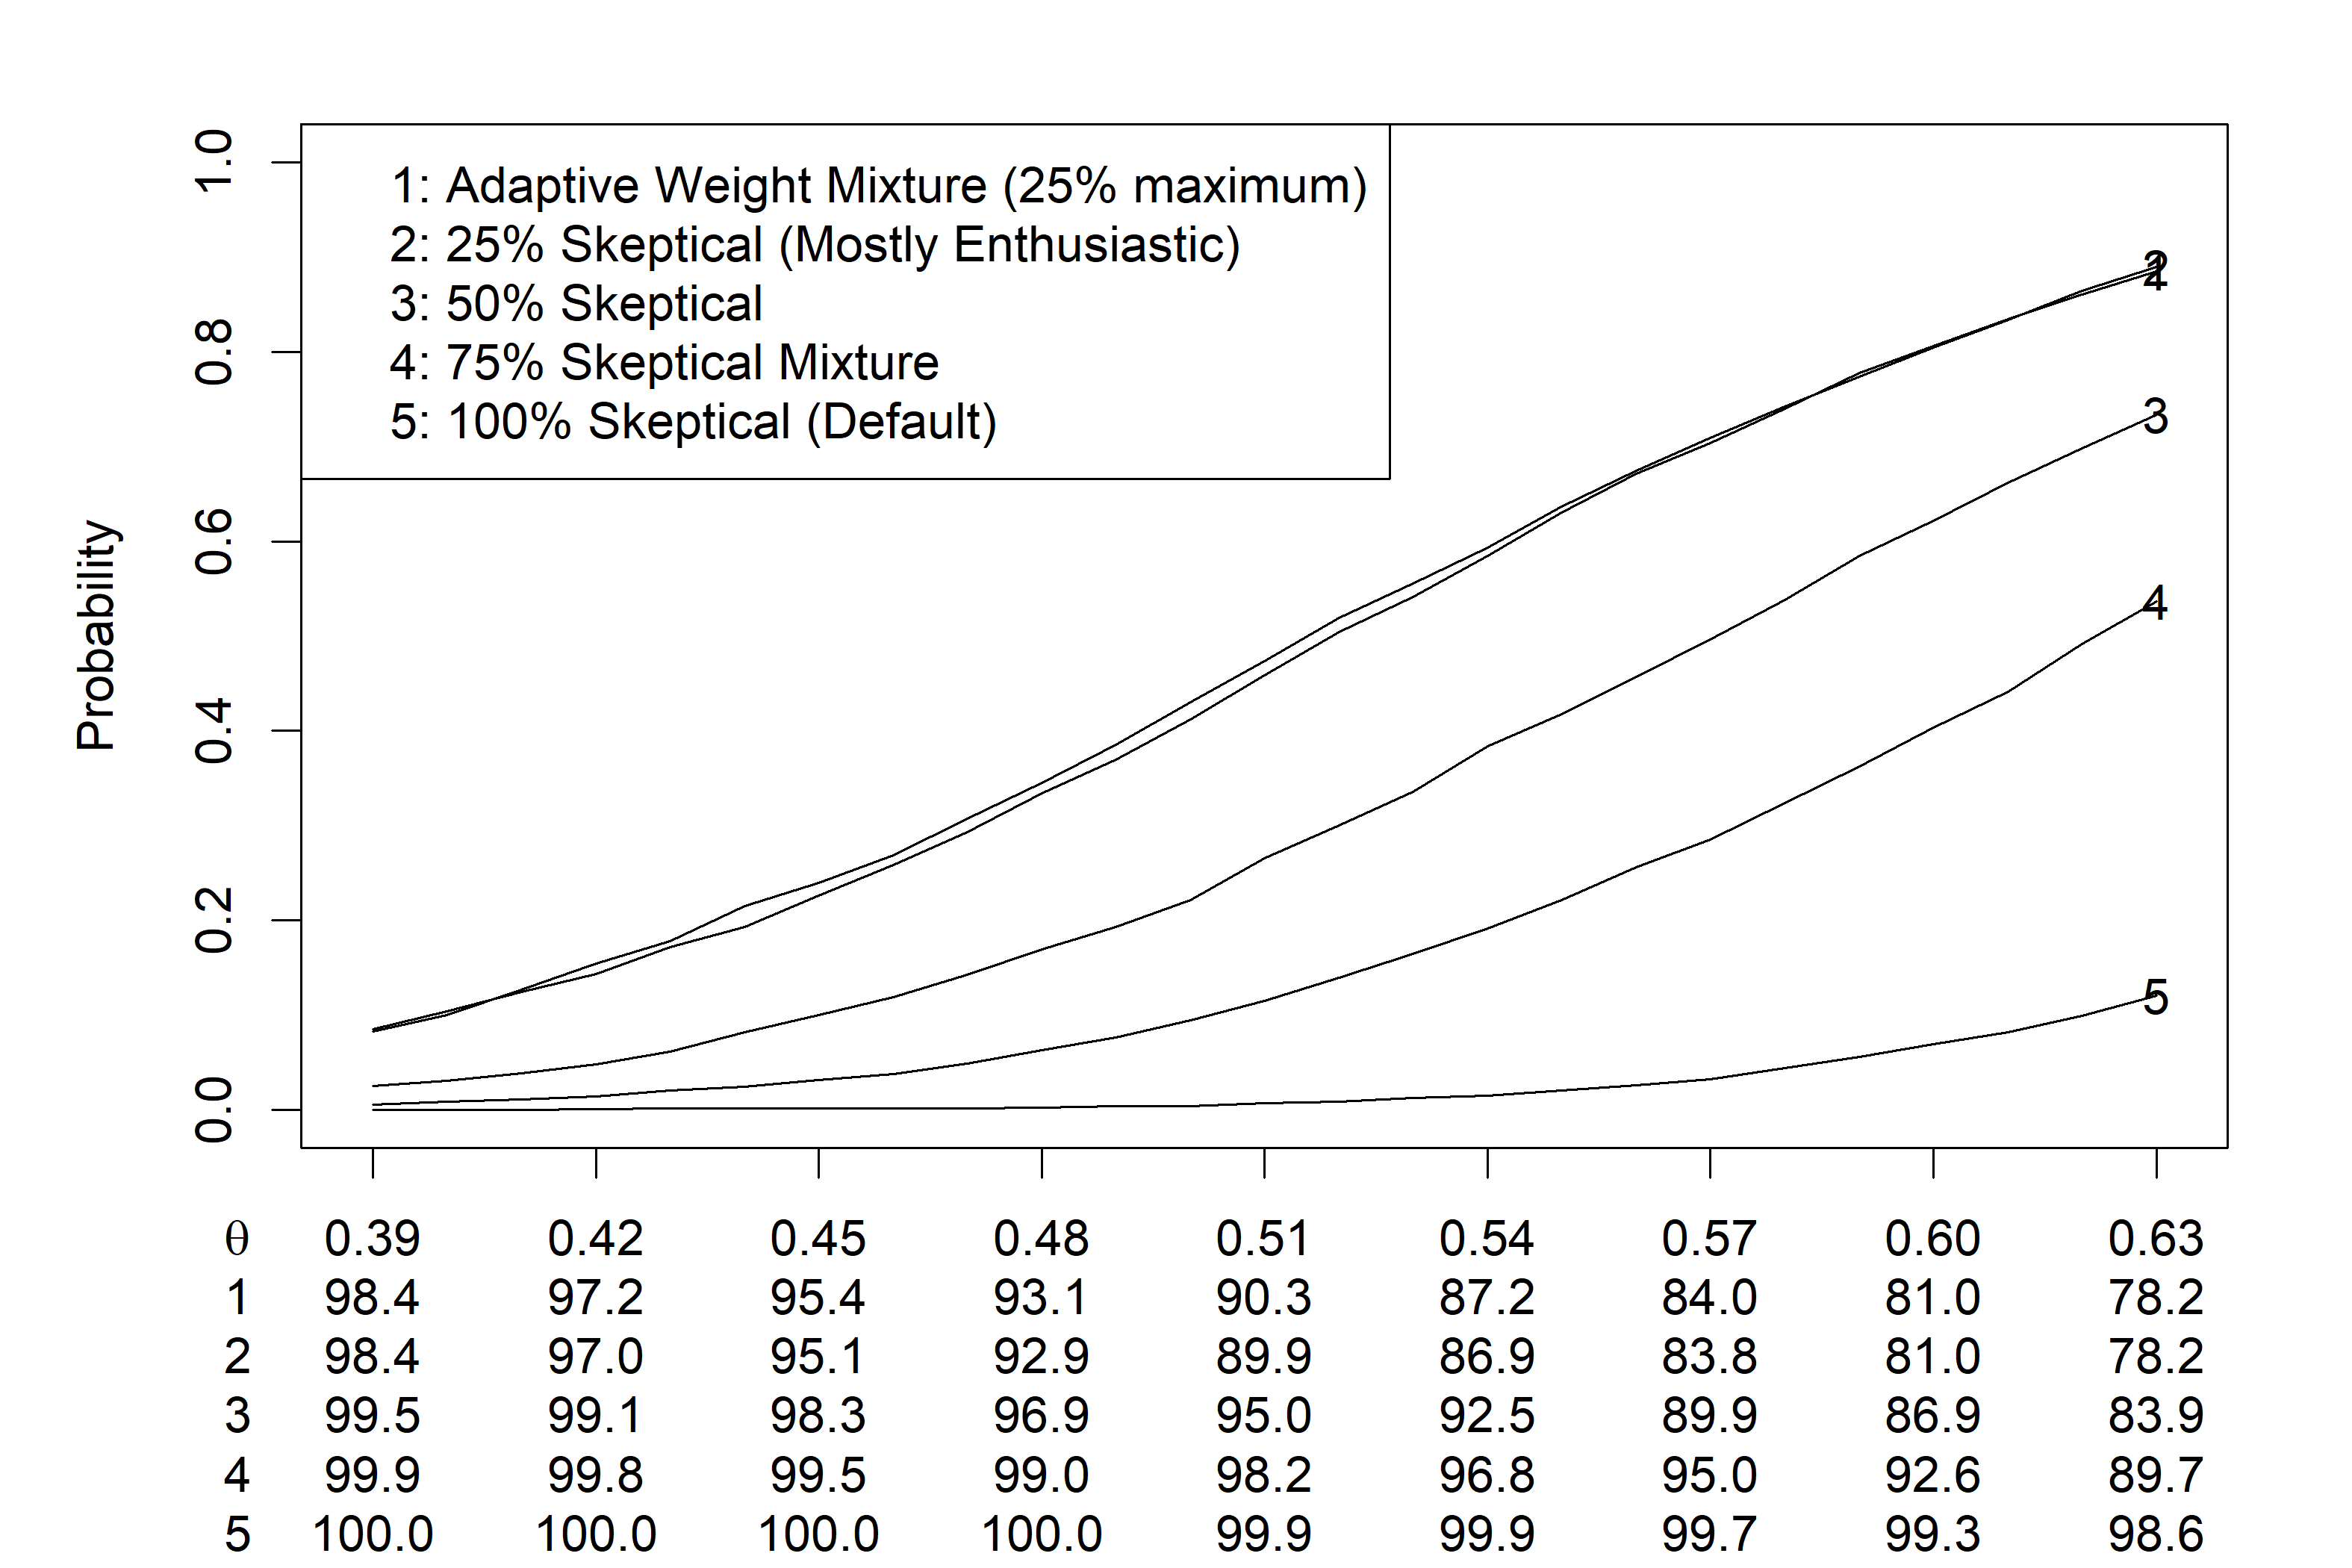
\includegraphics[width=6in]{figure6.png}
    \caption{A, Sequential design properties using adaptive weight monitoring prior. (SS; sample size, PM; posterior mean, CP; coverage probability, (I); interim analysis, (F); final analysis). B, Probability of stopping for efficacy and associated sample sizes by true IP response rate $\theta$ with different choices of efficacy monitoring prior.}
\label{fig:ex2varyomega}
 \end{center}
\end{figure}

Figure \ref{fig:3-part-compatibility}(A) shows the prior-data compatibility assessments $\psi^{(S)}$, $\psi^{(E)}$, $\psi^{(NI)}$ by observed risk difference. As expected, the skeptical and enthusiastic priors show highest compatibility when the observed risk difference matches the corresponding prior mode, and the non-informative prior shows high compatibility for a wide range of $\theta$. Figure \ref{fig:3-part-compatibility}(B) shows the 3-part mixture inference prior weights $\omega_S$, $\omega_{E}$, $\omega_{NI}$ using \eqref{eq:3partmix}-\eqref{eq:3partmix_ni} by observed risk difference. Recall our goal is to create a mixture prior which favors the skeptical or enthusiastic components in areas where high compatibility is demonstrated for those components, and favors the locally non-informative prior if both the skeptical and enthusiastic components show low compatibility. To this end, the skeptical and enthusiastic components have the highest weight when the observed data is aligned with the prior mode, and the locally non-informative prior has highest weight towards extreme values of the observed response difference.


\begin{figure}\begin{center}
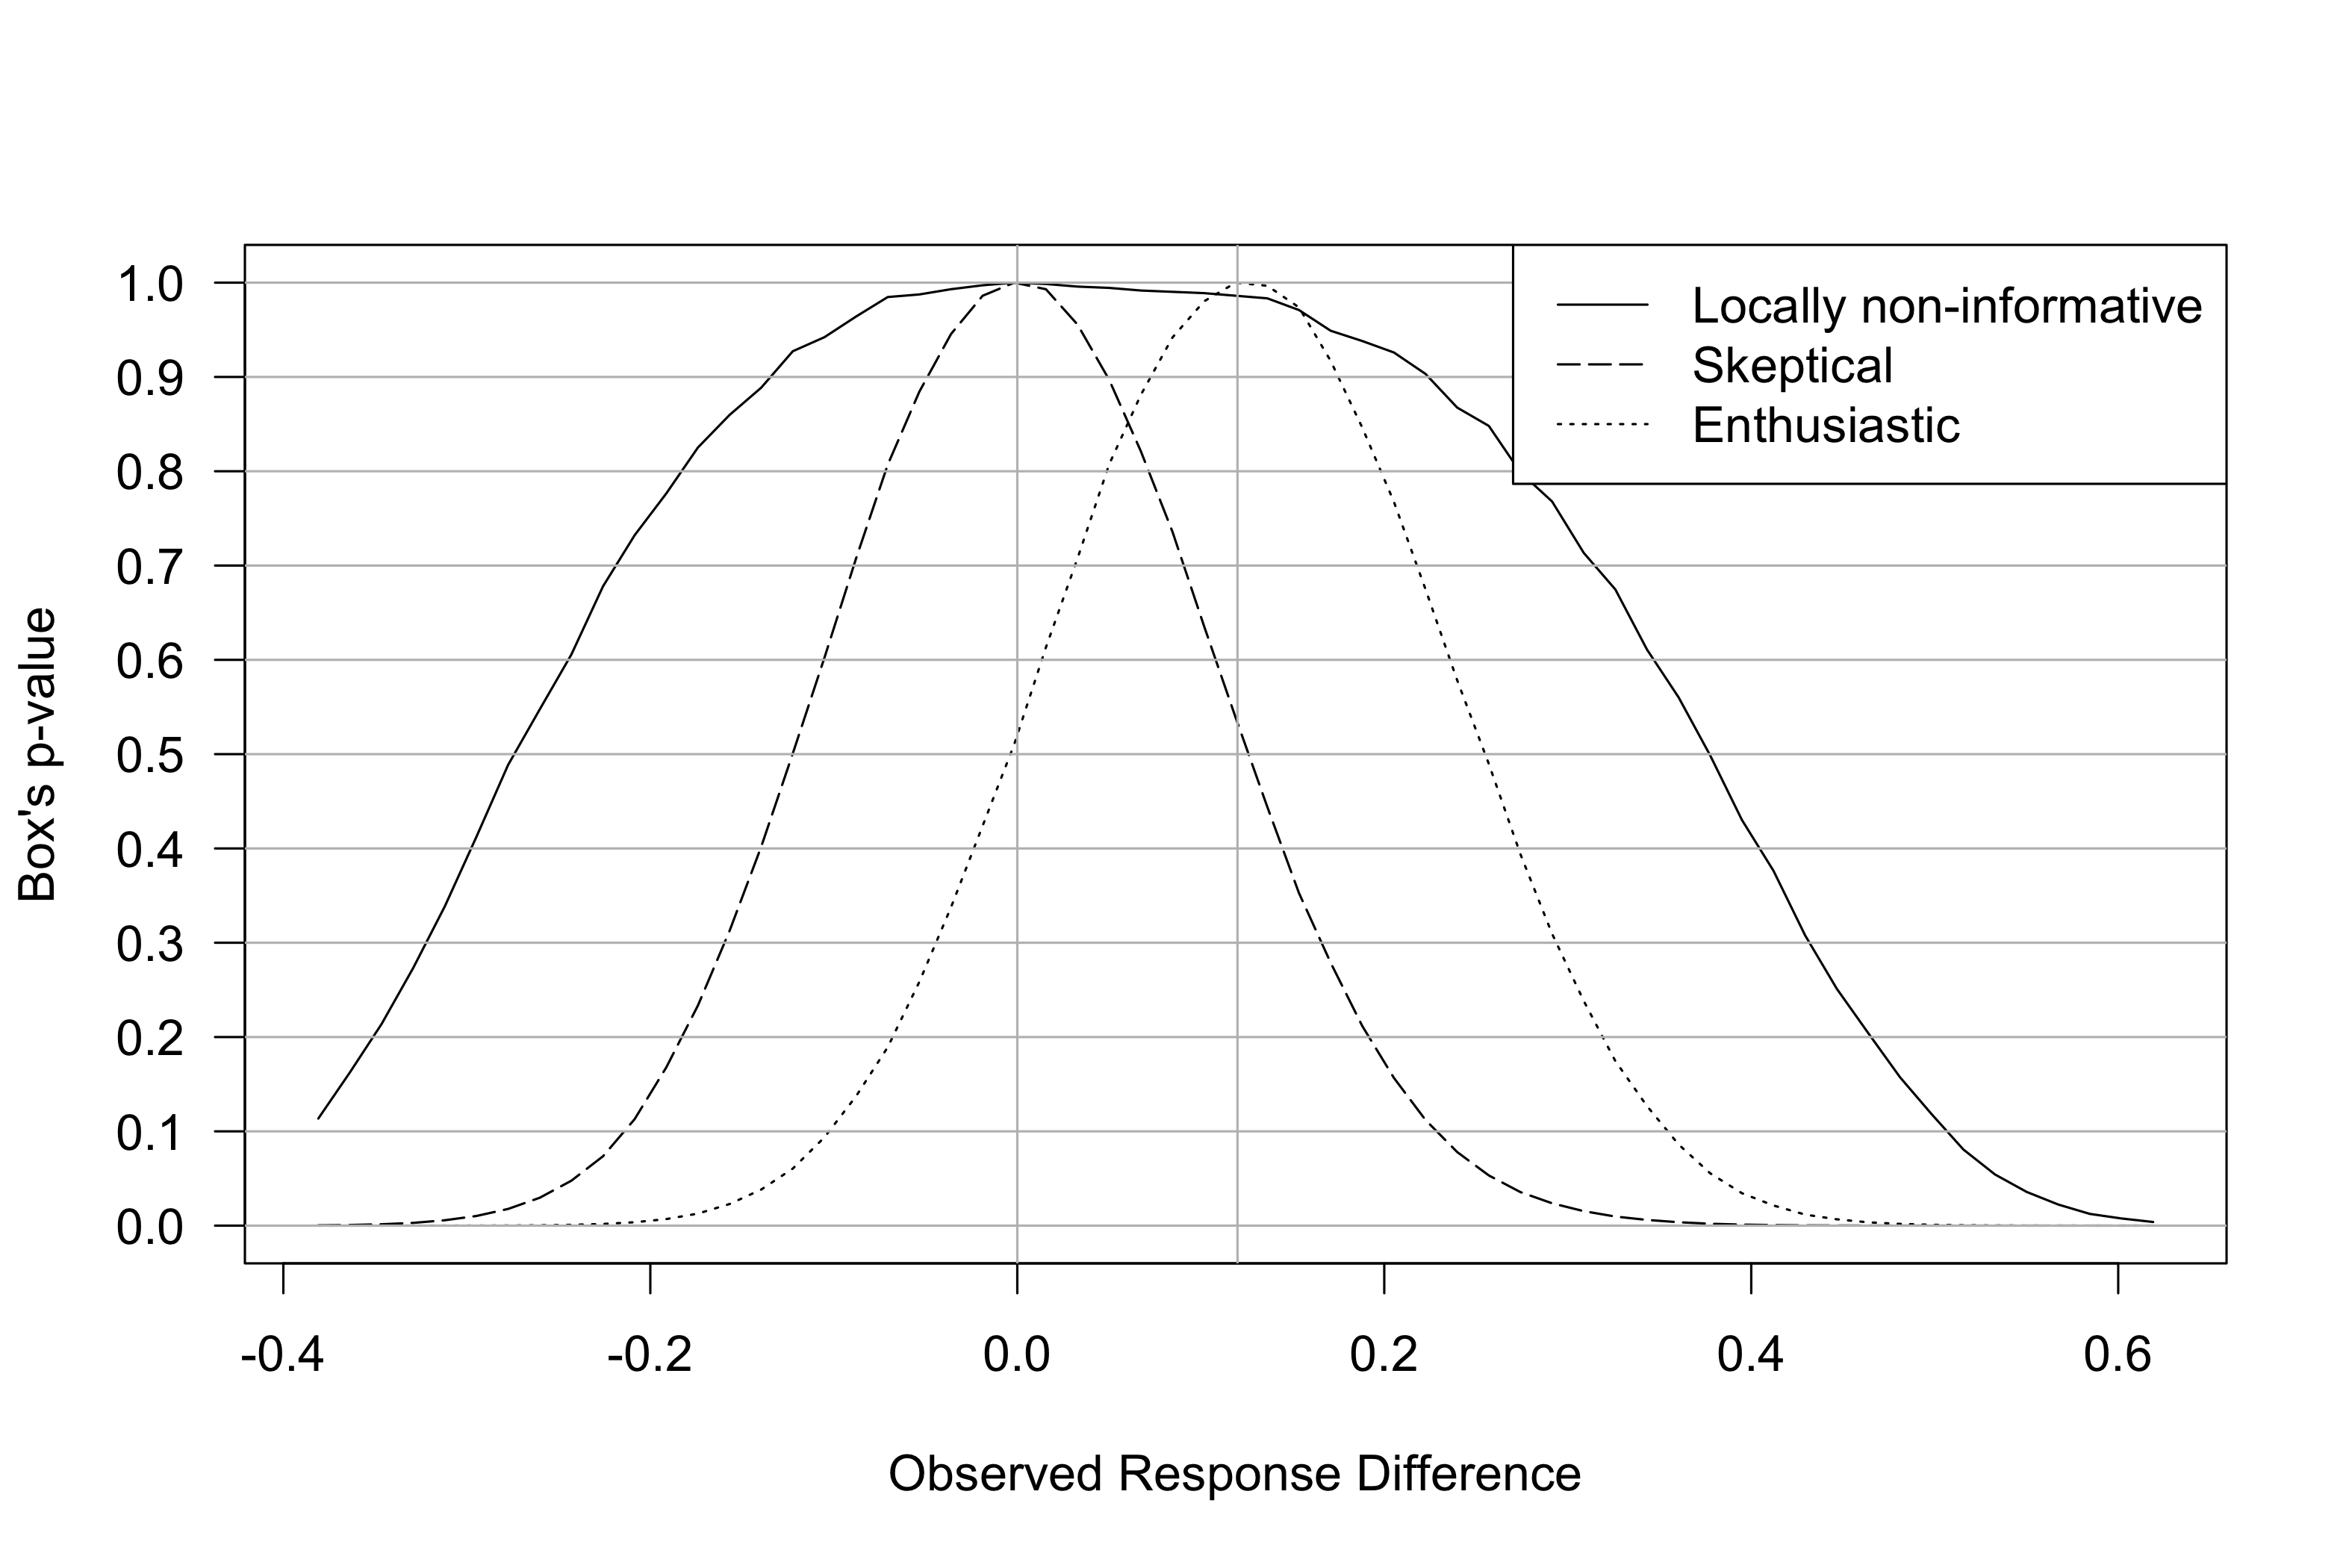
\includegraphics[width=6in]{3-part-compatibility-1.png}
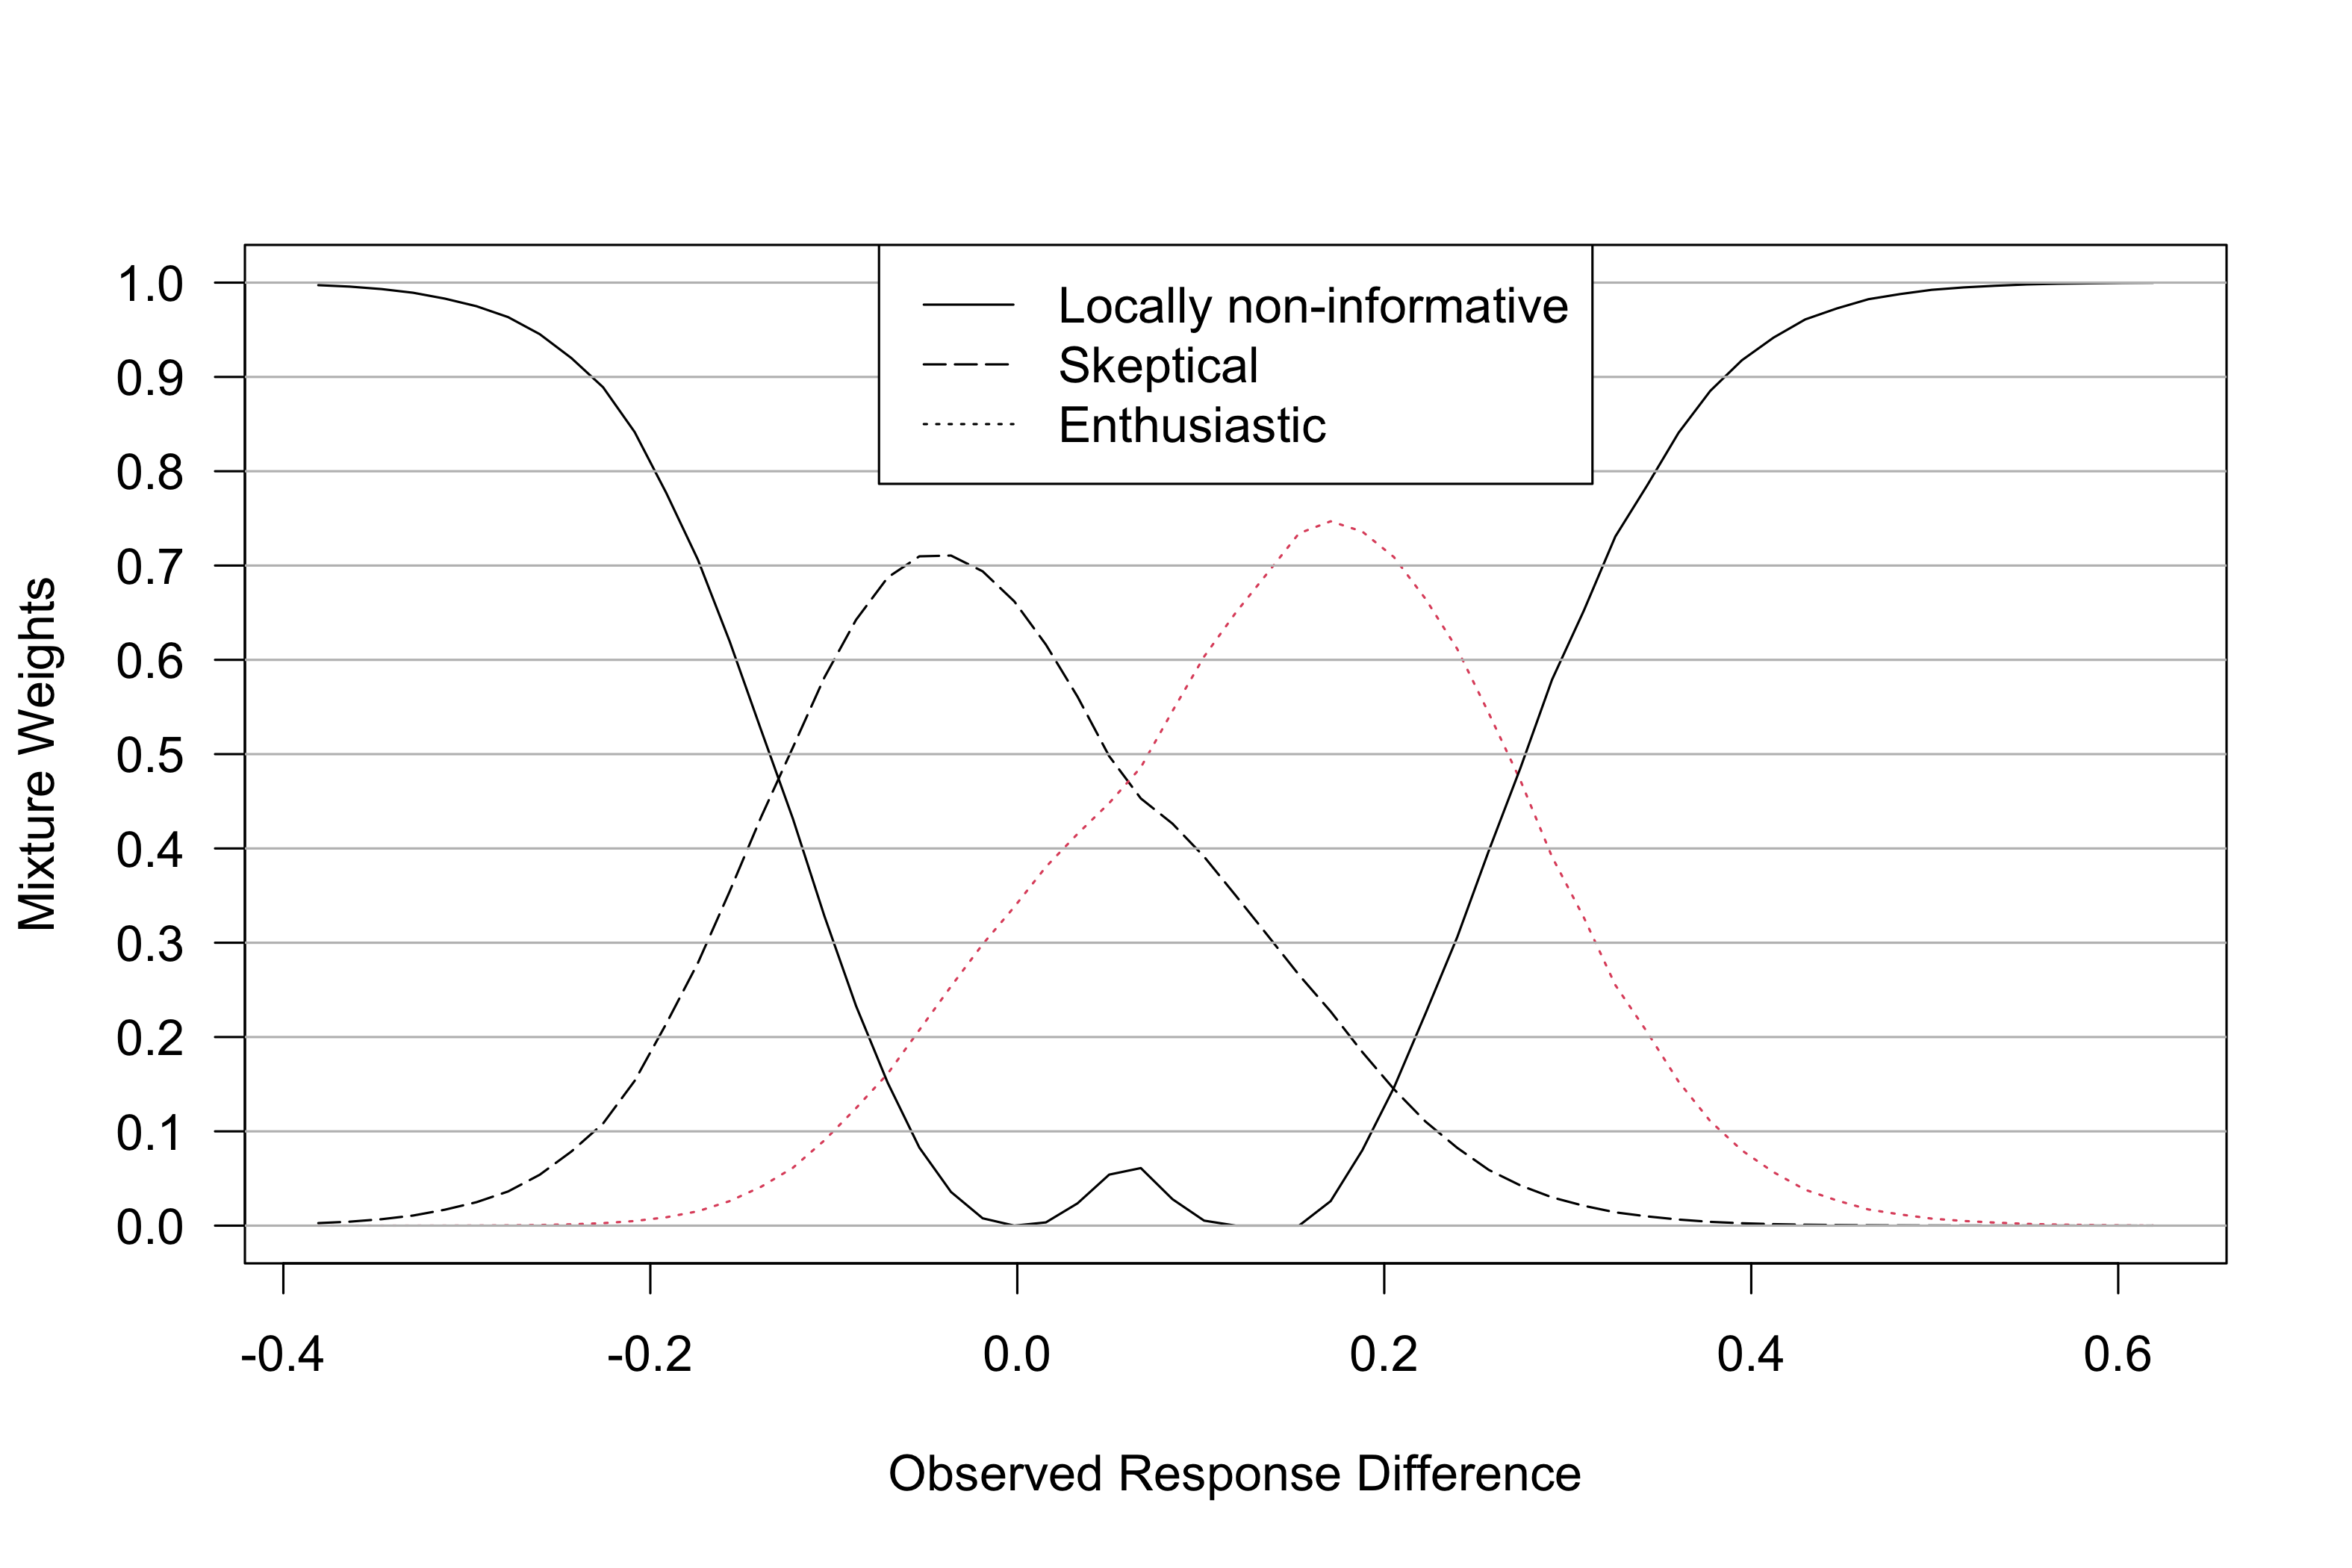
\includegraphics[width=6in]{3-part-compatibility-2.png}
    \caption{A; Prior-data compatibility assessments $\psi^{(S)}$, $\psi^{(E)}$, $\psi^{(NI)}$ by observed risk difference. B; 3-part mixture inference prior weights $\omega_S$, $\omega_{E}$, $\omega_{NI}$ by observed risk difference.}
\label{fig:3-part-compatibility}
 \end{center}
\end{figure}

\section{Discussion}
Bayesian methods are well suited for sequentially monitored clinical trials because of their natural interpretations and ability to incorporate external evidence through prior distributions. Monitoring priors used for efficacy and futility stopping fundamentally determine the operating characteristics of the trial, in addition to factors such as the frequency of data monitoring and number of patients in progress at enrollment termination. 

This paper presents a structured framework for designing a Bayesian sequentially monitored clinical trial. The generalized normal distribution gives a flexible and intuitive way to create monitoring priors. It is required that the practitioner specify the modal value, a quantile condition, and an additional parameter which can concentrate or flatten the distribution around the modal value (with the normal distribution as the default case). This paper demonstrates how the operating characteristics are affected by the choice of monitoring priors.

Presentation of these concepts was simplified by generic choices for design parameters. The same quantity $1-\epsilon$ was used as the threshold for substantial evidence in efficacy and futility monitoring \eqref{eq:eff_evidence} and \eqref{eq:fut_evidence}. In practice, the value of $\epsilon$ could be different for these two purposes (e.g. $\epsilon_{\text{eff}}=0.025$, $\epsilon_{\text{fut}}=0.05$). The intermediate effect size $\theta_m$ used in futility monitoring \eqref{eq:futility_criteria} was chosen to be $\theta_m=(\theta_0+\theta_1)/2$, but another effect size between $\theta_0$ and $\theta_1$ could be considered. Different assessments of prior-data conflict could be used to create a dynamic prior \eqref{eq:inference_prior}. Other distributions than the generalized normal could be used to create monitoring priors with the desired modal value and tail probability constraint (Section \ref{sec:gen_normal}). Each of these quantities could be modified to better suit the needs of the practitioner. 

Although the examples provided are superiority trials with binary data and response probabilities as the parameter of interest, the framework applies to any type of data likelihood and parameter of interest on an interval domain. Future work will involve demonstrating the framework in Bayesian clinical trials with survival outcomes.

%\begin{table}
%\caption{This is a simple table.}
%\label{t:one}
%\begin{center}
%\begin{tabular}{lrrr}
%\Hline
%Estimator & \multicolumn{1}{c}{$\beta_1$} &  \multicolumn{1}{c}{$\beta_2$} & 
%\multicolumn{1}{c}{$\beta_3$} \\ \hline
%MLE & 10.18 & $-$3.26 & 0.13 \\
%OLS & 9.92 & $-$3.19 & 0.11 \\
%WLS & 9.88 & $-$3.33 & 0.12 \\
%\hline
%\end{tabular}
%\end{center}
%\end{table}

%  The \backmatter command formats the subsequent headings so that they
%  are in the journal style.  Please keep this command in your document
%  in this position, right after the final section of the main part of 
%  the paper and right before the Acknowledgements, Supporting Information (Supplementary %  Materials),   and References sections. 

\backmatter

%  This section is optional.  Here is where you will want to cite
%  grants, people who helped with the paper, etc.  But keep it short!

\section*{Acknowledgements}

\vspace*{-8pt}



%  Here, we create the bibliographic entries manually, following the
%  journal style.  If you use this method or use natbib, PLEASE PAY
%  CAREFUL ATTENTION TO THE BIBLIOGRAPHIC STYLE IN A RECENT ISSUE OF
%  THE JOURNAL AND FOLLOW IT!  Failure to follow stylistic conventions
%  just lengthens the time spend copyediting your paper and hence its
%  position in the publication queue should it be accepted.

%  We greatly prefer that you incorporate the references for your
%  article into the body of the article as we have done here 
%  (you can use natbib or not as you choose) than use BiBTeX,
%  so that your article is self-contained in one file.
%  If you do use BiBTeX, please use the .bst file that comes with 
%  the distribution.  In this case, replace the thebibliography
%  environment below by 
%
\bibliographystyle{biom} 
\bibliography{fda_bib_062420}

%\begin{thebibliography}{}
%
%\bibitem{ } Cox, D. R. (1972). Regression models and life tables (with
%discussion).  \textit{Journal of the Royal Statistical Society, Series B}
%\textbf{34,} 187--200.
%
%\bibitem{ }  Hastie, T., Tibshirani, R., and Friedman, J. (2001). \textit{The 
%Elements of Statistical Learning: Data Mining, Inference, and Prediction}.
%New York: Springer.
%
%\end{thebibliography}

%  If your paper refers to supporting web material, then you MUST
%  include this section!!  See Instructions for Authors at the journal
%  website http://www.biometrics.tibs.org


%\section*{Supporting Information}

\vspace*{-8pt}

%\appendix

%  To get the journal style of heading for an appendix, mimic the following.

%\section{}
%\subsection{Title of appendix}

\section{Supplementary Material}

\subsection{Bayesian Hypothesis Testing}\label{sec:hypothesis}
Consider the hypotheses $H_0:\theta\in\Theta_{0}$ versus $H_1:\theta\in\Theta_{1}$ where $\Theta_{0}\bigcup \Theta_{1} = \Theta$ and $\Theta_{0} \bigcap \Theta_{1} = \emptyset$.
%
Formal Bayesian hypothesis testing requires the specification of prior probabilities on the hypotheses (e.g., $p(H_i)$ for $i=0,1$)
and prior distributions for $\left(\theta,\eta\right)$ specified over the parameter space defined with respect to each of the 
hypotheses (e.g. $\pi\left(\theta,\eta \big| H_i\right)$ for $i=0,1$). 
%

The posterior probability of hypothesis $H_i$ is given by 
\begin{equation}\label{eq:equation1}
p(H_i|\bmath{D})=\frac{p(\bmath{D}|H_i)\cdot p(H_i)}{p(\bmath{D}|H_0)\cdot p(H_0)+p(\bmath{D}|H_1)\cdot p(H_1)},
\end{equation}
where $p(\bmath{D}|H_i) = \int_{\Theta_i} p(\bmath{D}|\theta)\pi(\theta|H_i)d\theta$ is the marginal likelihood associated with hypothesis $H_i$.
%
In practice, most Bayesian methods for clinical trials perform hypothesis testing based on the posterior probability of the \textit{event defining $H_i$}.
%
For this approach, one simply needs to specify a prior $\pi\left(\theta\right)$ representing belief about $\theta$ overall and compute the posterior distribution.
%
The posterior probability that $\theta\in\Theta_i$ is given by
\begin{equation}\label{eq:equation2}
P(\theta\in\Theta_i|\bmath{D})
%=\frac{\int_{\Theta_i} p(\bmath{D}|\theta)\pi (\theta)d\theta}{\int_{\Theta}p(\bmath{D}|\theta)\pi(\theta) d\theta}
=\frac{\int_{\Theta_i} p(\bmath{D}|\theta)\pi (\theta|\theta\in\Theta_i)d\theta\cdot P(\theta\in\Theta_i)}
      { \sum_{j=0,1} \int_{\Theta_j}p(\bmath{D}|\theta)\pi (\theta|\theta\in\Theta_j)d\theta\cdot P(\theta\in\Theta_j) }
\end{equation}
where $P(\theta\in\Theta_i)=\int_{\Theta_i}\pi(\theta)d\theta$. 
%
We can readily see that the $P(\theta\in\Theta_i|\bmath{D})$ is equal to $p(H_i|\bmath{D})$ if one takes
$p(H_i) =P(\theta\in\Theta_i)$ and $\pi\left(\theta \big| H_i\right) = \pi\left(\theta\big|\theta \in \Theta_i\right)$ for $i=0,1$.
%
If in fact $\pi\left(\theta\right)$ does represent belief about $\theta$, these choices are perhaps the most intuitive and thus 
we should have no reservation referring to $P(\theta\in\Theta_i|\bmath{D})$ as the probability that hypothesis $H_i$ is true.
\subsection{Monitoring Prior Parameterization}\label{sec:gen_normal_details}

\subsubsection{Normal Distribution $\mathcal{N}_p(\tilde{\mu},q)$}\label{sec:normal_tail_area}
%The specification of the mean and variance of a normal distribution completely specifies the modal value and a tail-probability constraint, and is therefore sufficient for defining enthusiastic and skeptical priors.

Suppose $\theta\sim\mathcal{N}(\mu,\sigma)$ is a normal random variable that satisfies $\rmn{mode}(\theta)=\tilde{\mu}$ and $P(\theta\leq q)=p$. The values for the mean and standard deviation are $\mu=\tilde{\mu}$ and $\sigma=\frac{q-\mu}{\Phi^{-1}(p)}$, where $\Phi$ denotes the cumulative distribution function for a standard normal distribution and $\Phi^{-1}$ denotes its quantile function. Therefore we can denote the distribution with the desired mode and tail probability constraint as  $\theta\sim\mathcal{N}_p(\tilde{\mu},q)$, which is well-defined for values $(\mu,q,p)$ that satisfy $\frac{q-\mu}{p-0.5}>0$. Since the normal distribution is completely specified by $(\mu, \sigma)$, quantities such as $P(\theta\leq\tilde{q})$ are also specified for any $\tilde{q}\in\mathbb{R}$. In particular, if $\theta\sim\mathcal{N}_p(\tilde{\mu},q)$ then $P(\theta\leq\frac{q+\mu}{2})=\Phi(\frac{\Phi^{-1}(p)}{2})$. Furthermore, $P(\theta\in(\mu,\frac{q+\mu}{2}))=|p-\Phi(\frac{\Phi^{-1}(p)}{2})|$. 

\subsubsection{Generalized Normal Distributions $\mathcal{GN}_p(\tilde{\mu},q,\gamma)$}\label{sec:gen_norm_appendix}
Let $F_{\mu,\alpha,\beta}$ denote the cumulative distribution function of $\mathcal{GN}(\mu,\alpha,\beta)$. The CDF of a generalized normal random variable $\theta\sim\mathcal{GN}(\mu,\alpha,\beta)$ can be expressed as \citep{Griffin2018}
\begin{equation}
P(\theta\leq q|\mu,\alpha,\beta)=\frac{1}{2}+\frac{\rmn{sign}(q-\mu)}{2}\int_0^{|q-\mu|^\beta}\frac{w^{1/\beta-1}}{\alpha\Gamma(1/\beta)}\rmn{exp}\left\{-\left(\frac{1}{\alpha}\right)^\beta w\right\} dw
\end{equation}
%Computations involving $F_{\mu,\alpha,\beta}$ are done using the gnorm package \citep{Griffin2018}. 
Define $\theta\sim\mathcal{GN}_p(\tilde{\mu},q,\gamma)$ as the generalized normal distribution $\mathcal{GN}(\mu,\alpha,\beta)$ that satisfies mode$(\theta)=\tilde{\mu}$, $P(\theta\leq q)=p$, and $P(\theta\in(q,\frac{q+\mu}{2}))=\gamma\cdot|p-\Phi(\frac{\Phi^{-1}(p)}{2})|$.
%\end{mydef}
%
The mode is equal to $\mu=\tilde{\mu}$, and $\alpha$ and $\beta$ are determined to minimize the function $(F_{\mu,\alpha,\beta}(q)-p)^2+(F_{\mu,\alpha,\beta}(\frac{q+\mu}{2})-\gamma\cdot|p-\Phi(\frac{\Phi^{-1}(p)}{2})|)^2$ with box-constrained optimization \citep{Byrd1995}. %The restrictions on well-defined choices of $(p,\tilde{\mu},q,\gamma)$ for the $\theta\sim\mathcal{GN}_p(\tilde{\mu},q,\gamma)$ distribution are described in the appendix.

Using this notation to define the distributions in Figure \ref{fig:figure1} yields the default enthusiastic prior as $\mathcal{GN}_{p=0.025}(\tilde{\mu}=\theta_1,q=\theta_0,\gamma=1)$, the concentrated enthusiastic prior as $\mathcal{GN}_{p=0.025}(\tilde{\mu}=\theta_1,q=\theta_0,\gamma=0.75)$, the flattened enthusiastic prior as $\mathcal{GN}_{p=0.025}(\tilde{\mu}=\theta_1,q=\theta_0,\gamma=1.5)$, and the locally non-informative prior as $\mathcal{GN}_{p=0.025}(\tilde{\mu}=\frac{\theta_0+\theta_1}{2},q=\frac{3\theta_0-\theta_1}{2},\gamma=1.5)$.
\subsubsection{Truncated Generalized Normal Distribution $\mathcal{GN}_{p,\Theta}(\tilde{\mu},q,\gamma)$}\label{sec:gen_normal_appendix}
The density for a generalized normal distribution truncated to the interval domain $\Theta=(\theta_{min},\theta_{max})$, denoted by $\mathcal{GN}_\Theta(\mu,\alpha,\beta)$, is $f(\theta)=c\cdot\exp\left\{-\frac{|\theta-\mu|}{\alpha}^{\beta}\right\}{I(\theta\in \Theta)}$ where $c=\frac{\beta}{2\alpha \Gamma(1/\beta)}({F_{\mu,\alpha,\beta}(\theta_{max})-F_{\mu,\alpha,\beta}(\theta_{min})})^{-1}$. 
%\begin{mydef}\label{def:gennormaltruncated}
Define $\theta\sim\mathcal{GN}_{p,\Theta}(\tilde{\mu},q,\gamma)$ as the truncated generalized normal distribution $\mathcal{GN}_\Theta(\mu,\alpha,\beta)$ that satisfies mode$(\theta)=\tilde{\mu}$, $P(\theta\leq q)=p$, and $P(\theta\in(q,\frac{q+\mu}{2}))=\gamma|p-\Phi(\frac{\Phi^{-1}(p)}{2})|$.

Using this notation to define the distribution in Figure \ref{fig:figure5} yields the joint distribution $\pi(\theta,\eta)=\pi(\theta)\times\pi(\eta|\theta)$, as $
\pi(\theta)\sim\mathcal{GN}_{p=0.975,\Theta=[-1,1]}(\tilde{\mu}=\theta_0,q=\theta_1,\gamma=1)$ and $\pi(\eta|\theta)\sim \mathcal{GN}_{p=0.975,\Theta=[\rmn{max}(-\theta,0),\rmn{min}(1,1+\theta)]}(\tilde{\mu}=\eta_0,q=\eta_1,\gamma=1)$.

%\end{mydef}
%
%\subsection{Parameterizing the $\mathcal{GN}_p(\tilde{\mu},q,\gamma)$ Distribution}
%The restrictions on the choice of $(p,\tilde{\mu},q,\gamma)$ for the $\theta\sim\mathcal{GN}_p(\tilde{\mu},q,\gamma)$ distribution to be well-defined:

\subsection{Type 1 Error Rate Depending on Enrollment Schemes}
Recall Figure \ref{fig:ex1t1e} from Section \ref{sec:example1} which showed Type 1 error properties for the single-arm design. Figure \ref{fig:ex1t1e_longer} shows results from a design that has a longer follow-up period. The interim sample sizes are the same for each monitoring frequency, however, the final sample sizes under the longer follow-up designs are much larger (over 20 patients in follow-up for monitoring frequencies of 8 or fewer, compared to approximately 6 patients in the shorter follow-up designs). The final probability of efficacy criteria being satisfied is generally slightly lower in the longer follow-up design, which is what we would expect since the larger final sample size contains more data consistent with a null result.
\begin{figure}\begin{center}

   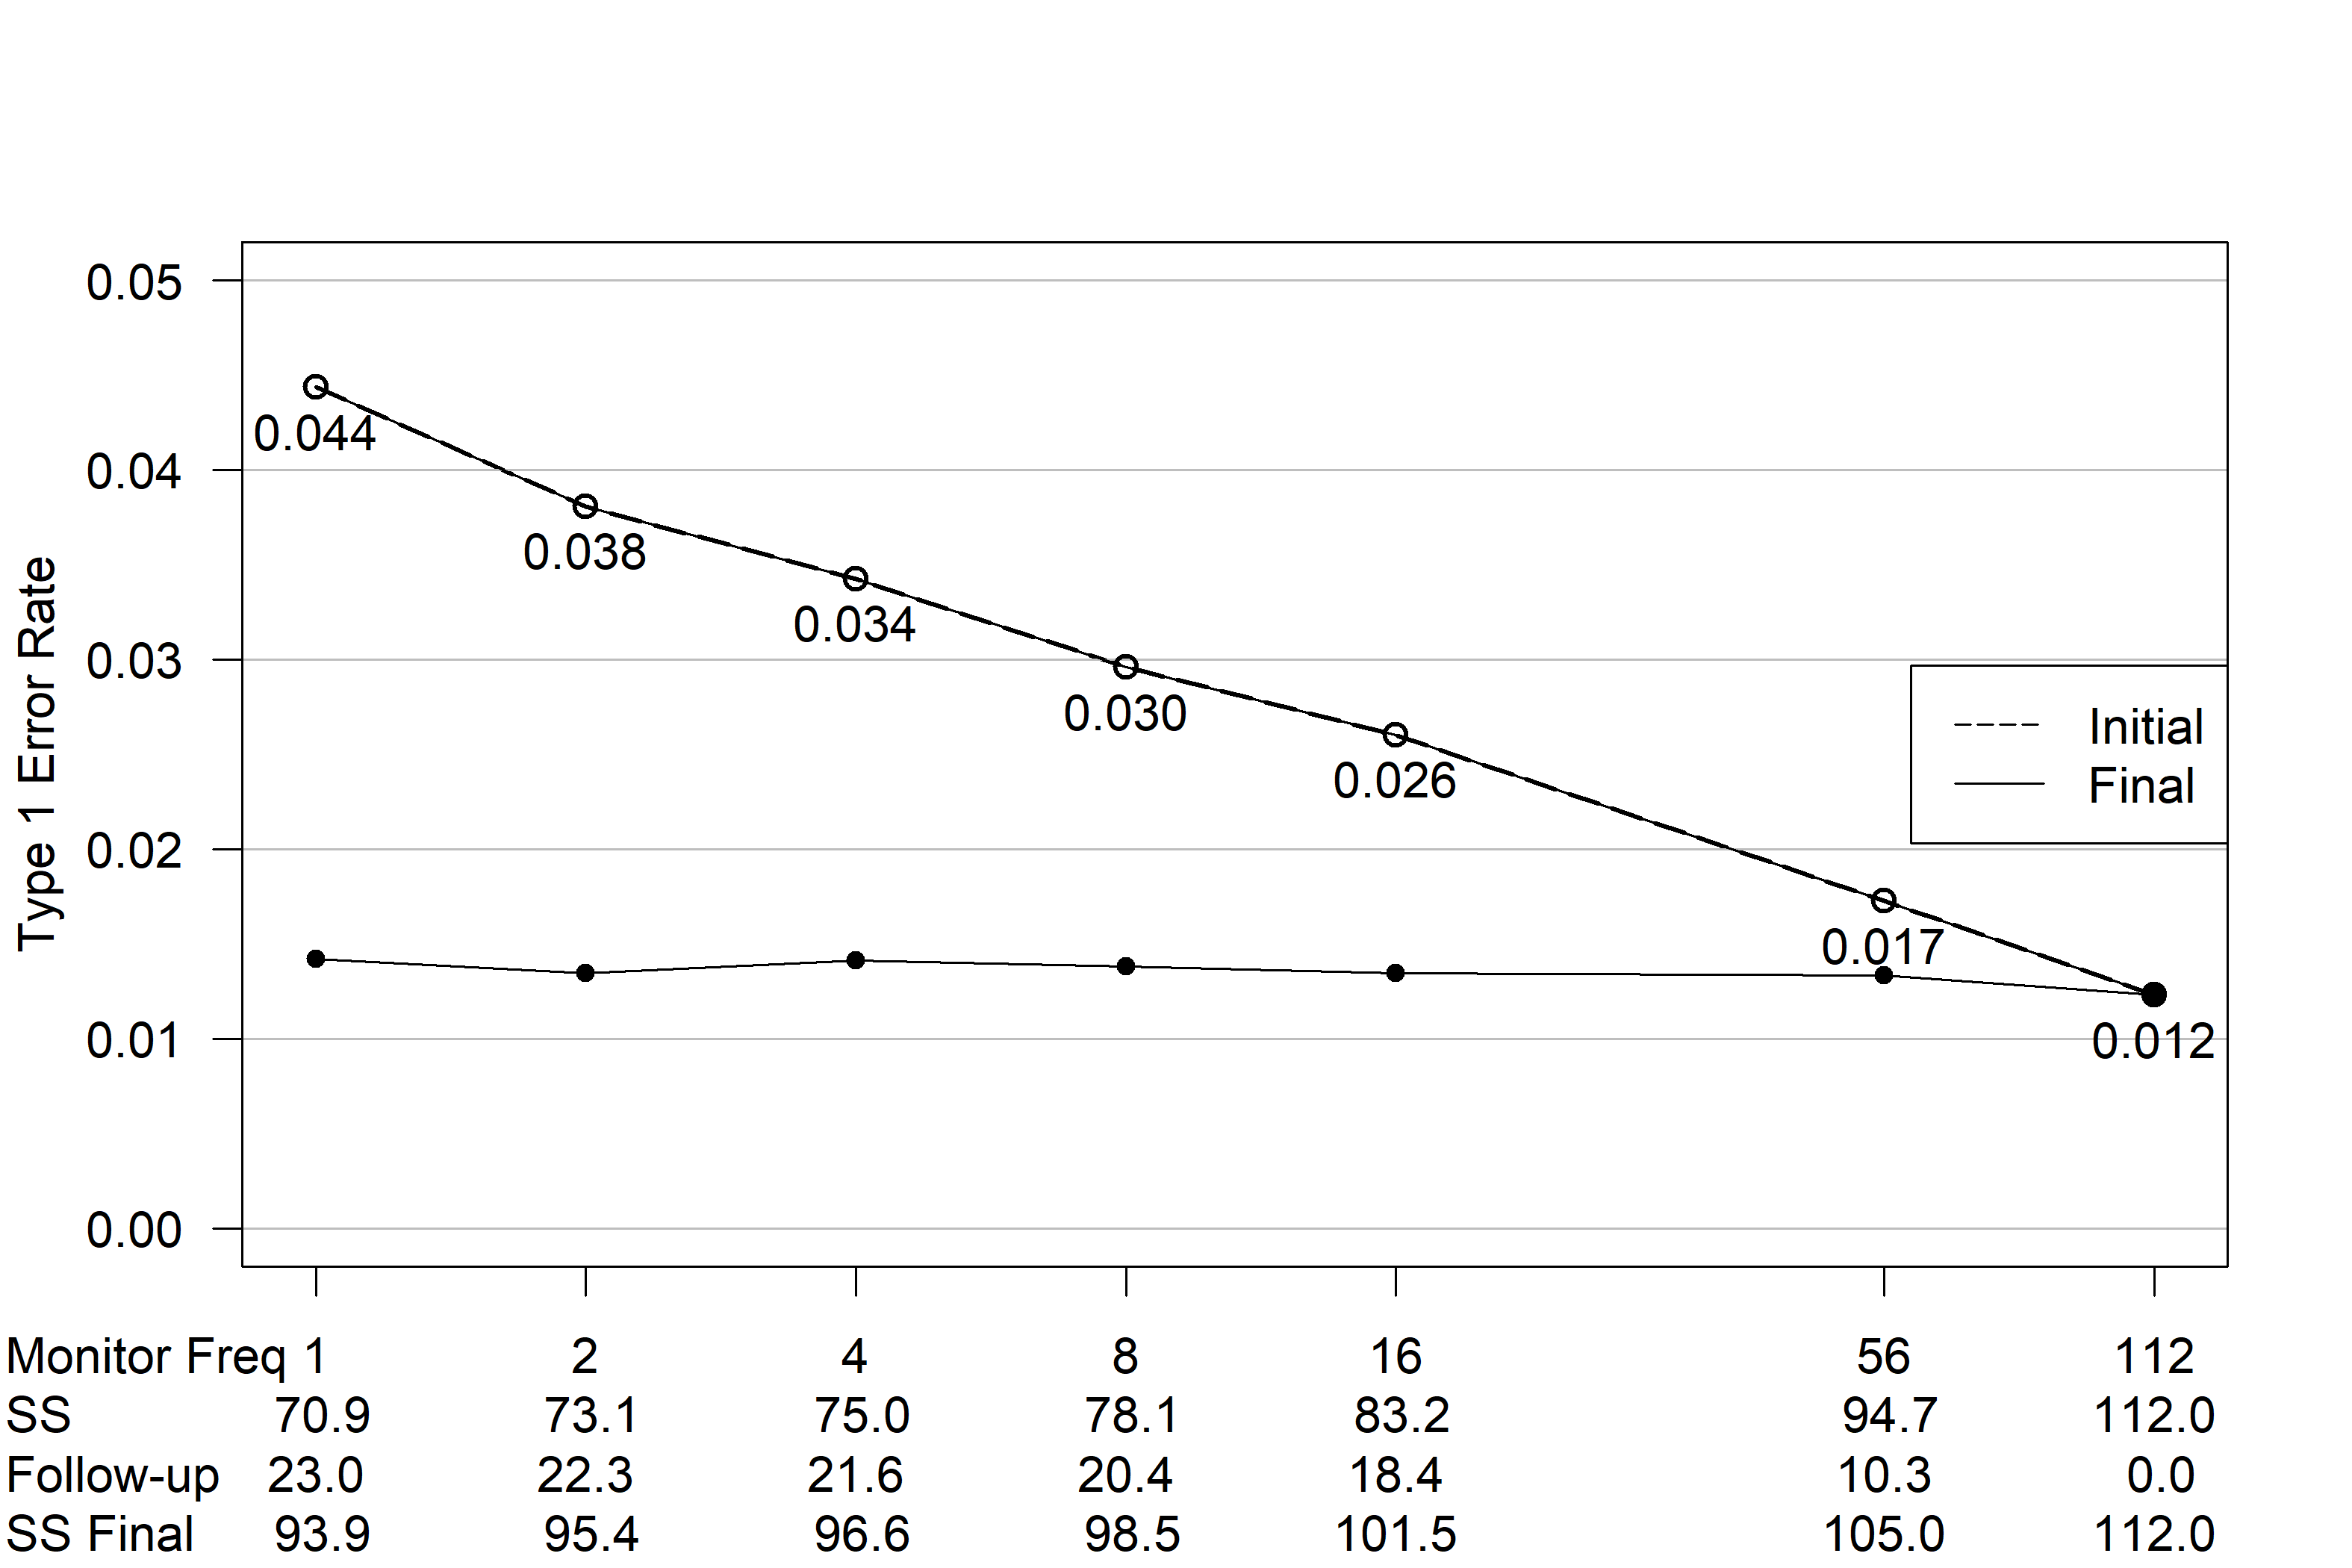
\includegraphics[width=6in]{figureS1.png}
    \caption{Single arm design from Example \ref{sec:example1} with a longer follow-up period. Probability of efficacy criteria being satisfied when $\theta=\theta_0$. SS; sample size. Monitor Freq; monitoring frequency.}
	\label{fig:ex1t1e_longer}

\end{center}
\end{figure}
\subsection{Robustness of Parameterizations of Monitoring Priors}\label{sec:priorRobustness}
The analyses done in Section \ref{sec:example1} used a concentrated skeptical prior and default enthusiastic prior. In this section we show the four possible designs using the combinations of skeptical and enthusiastic prior given in Figure \ref{fig:figure1}.

Figures \ref{fig:robustness1}-\ref{fig:robustness2} shows what happens when the enthusiastic prior shifts from default to flattened, with the skeptical prior remaining fixed. Note that in the region between $\theta_0$ and $\frac{\theta_0+\theta_1}{2}$ as the enthusiastic prior shifts from default to flattened, (a) the probability of stopping early for futility increases (b) the probability of inconclusive findings decreases and (c) the intermediate and final sample sizes decrease. This is because the enthusiastic prior gives more mass in for this region of $\theta$. The flattened enthusiastic prior was used in Section \ref{sec:example1} to enhance the ability of futility monitoring to reduce the sample size.

Contrasting \ref{fig:robustness1} and \ref{fig:robustness2}, we see that the probability of stopping early for efficacy is much higher at $\theta_0$ when the default skeptical prior is used rather than the concentrated skeptical prior. This is because the default skeptical prior has less mass around $\theta=\theta_0$, therefore it is easier to convince the skeptic that $\theta>\theta_0$ under the null result $\theta=\theta_0$. The concentrated skeptical prior was used in Section \ref{sec:example1} to limit this probability and provide better Type 1 error control.

The choice of skeptical and enthusiastic prior affects the analysis, and their specification (e.g. default, skeptical, enthusiastic) should be made with these properties in mind.

\begin{figure}\begin{center}

 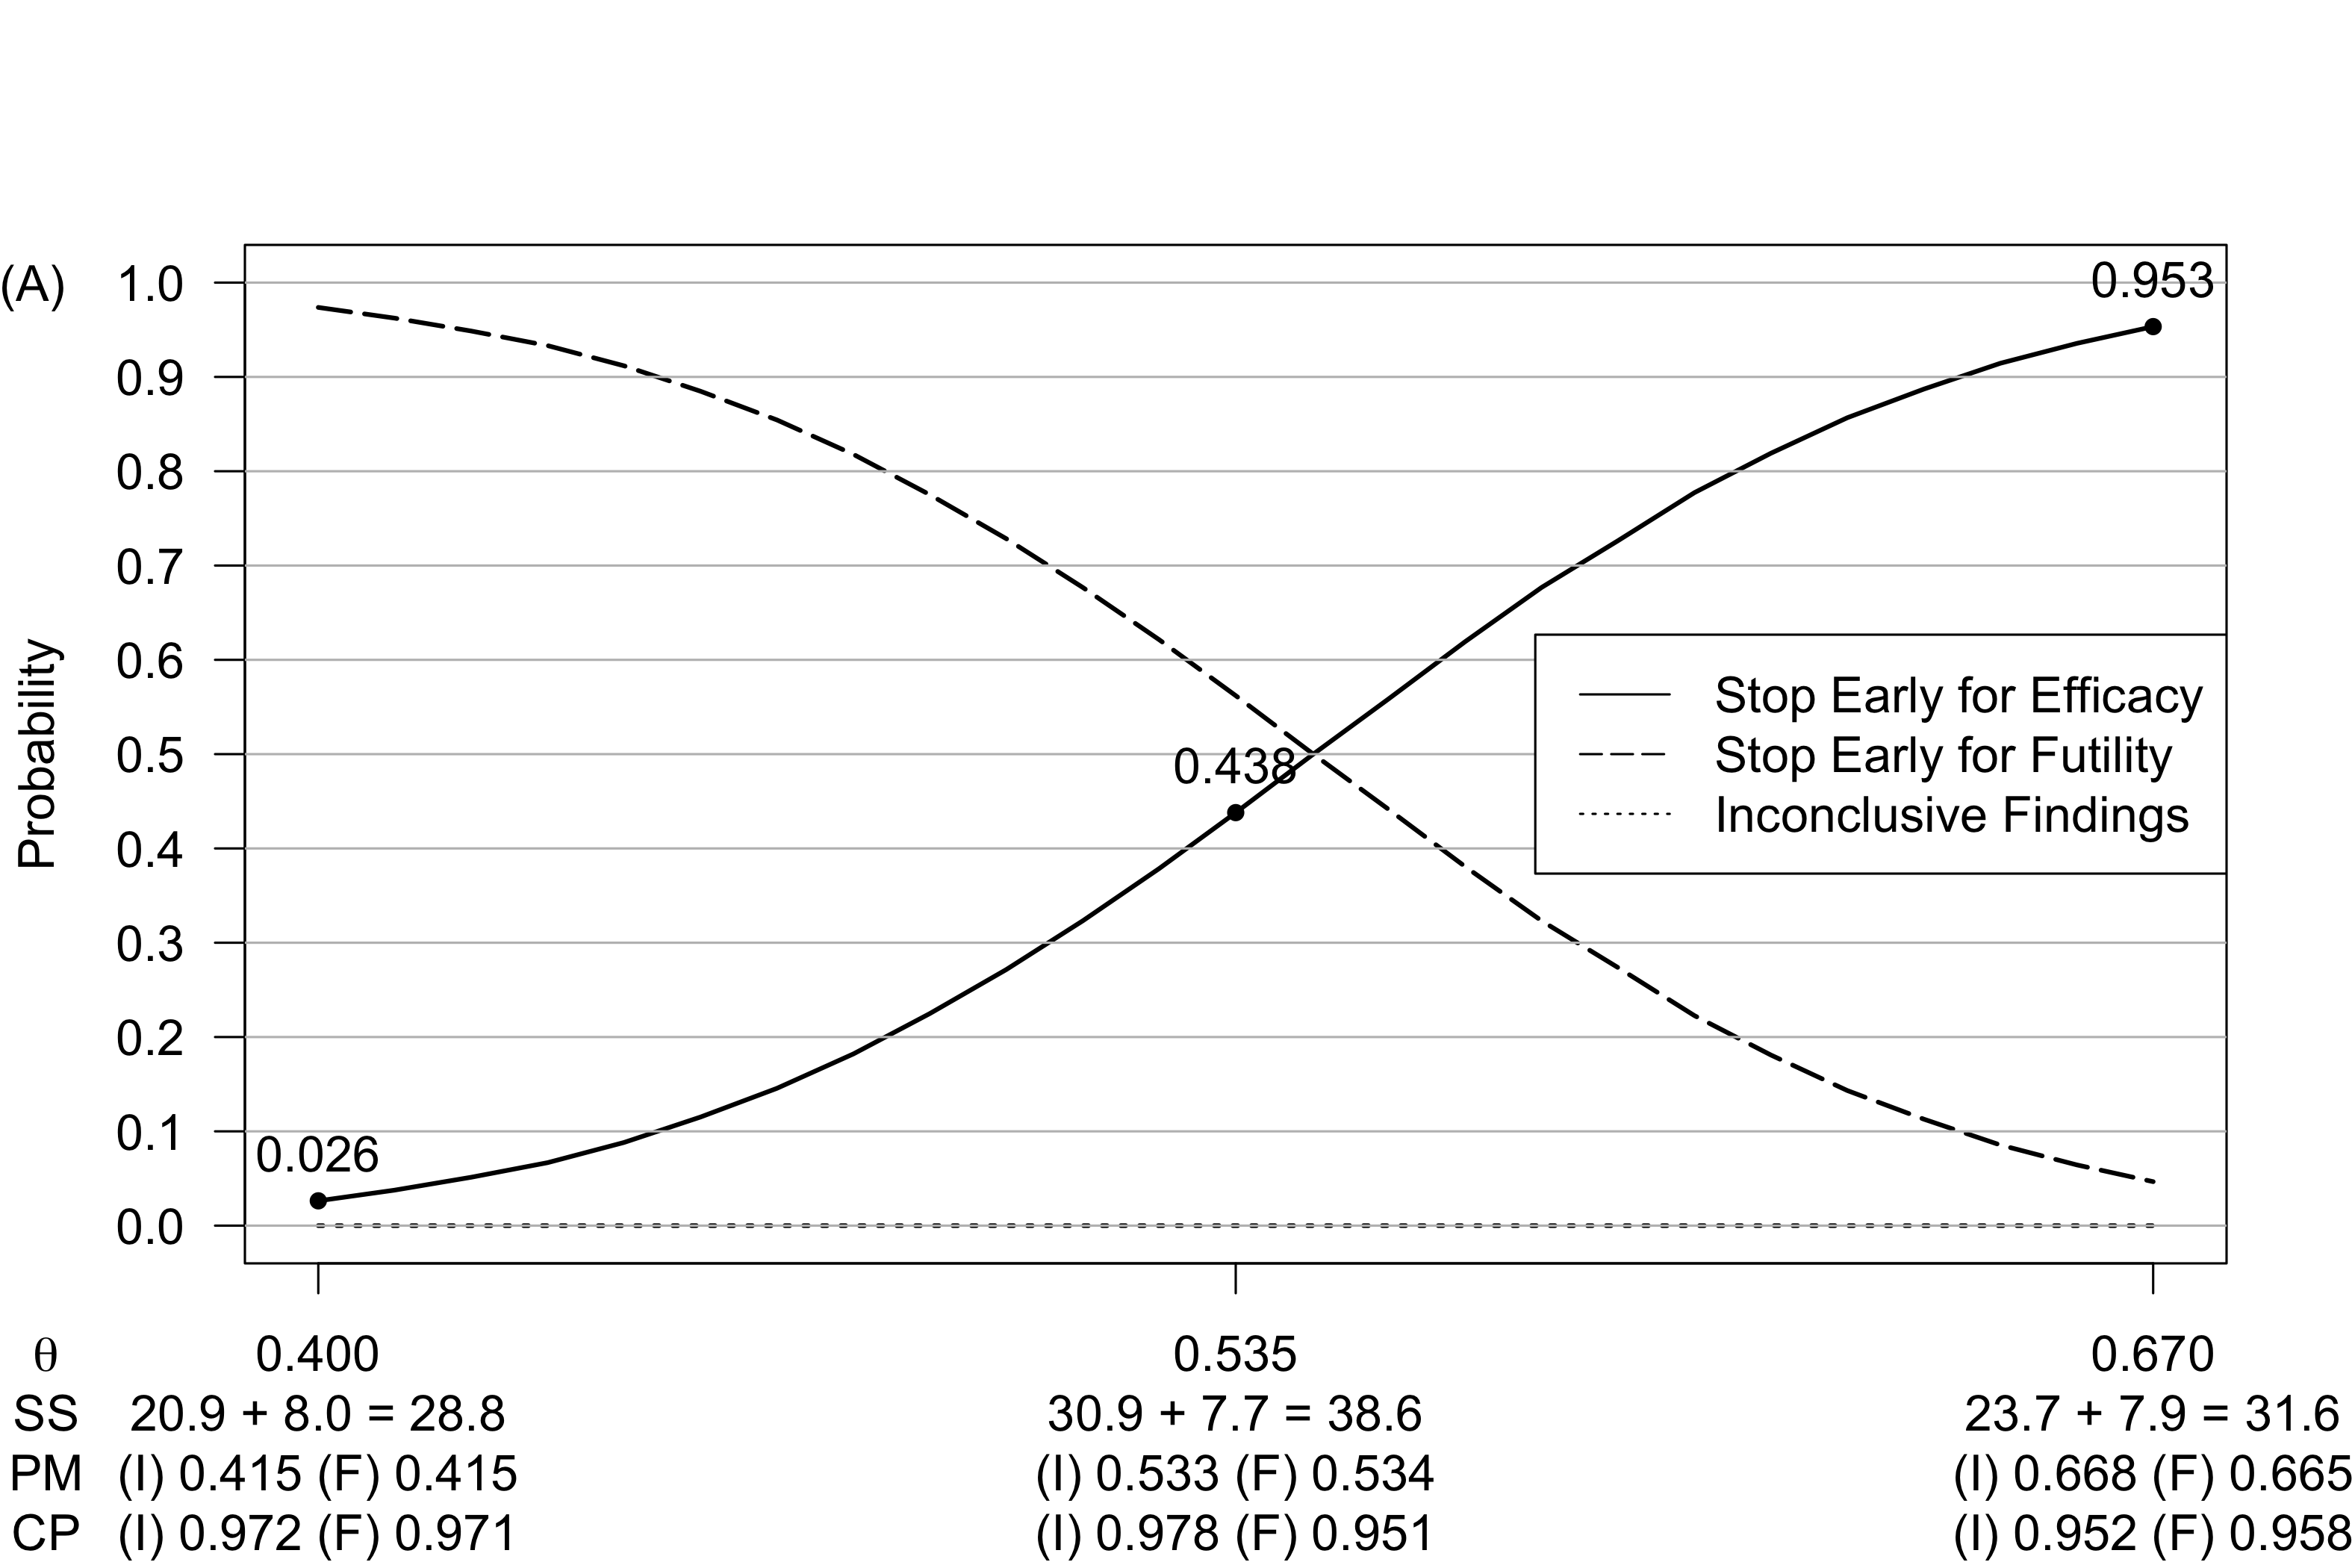
\includegraphics[width=6in]{figureS2a.png}
 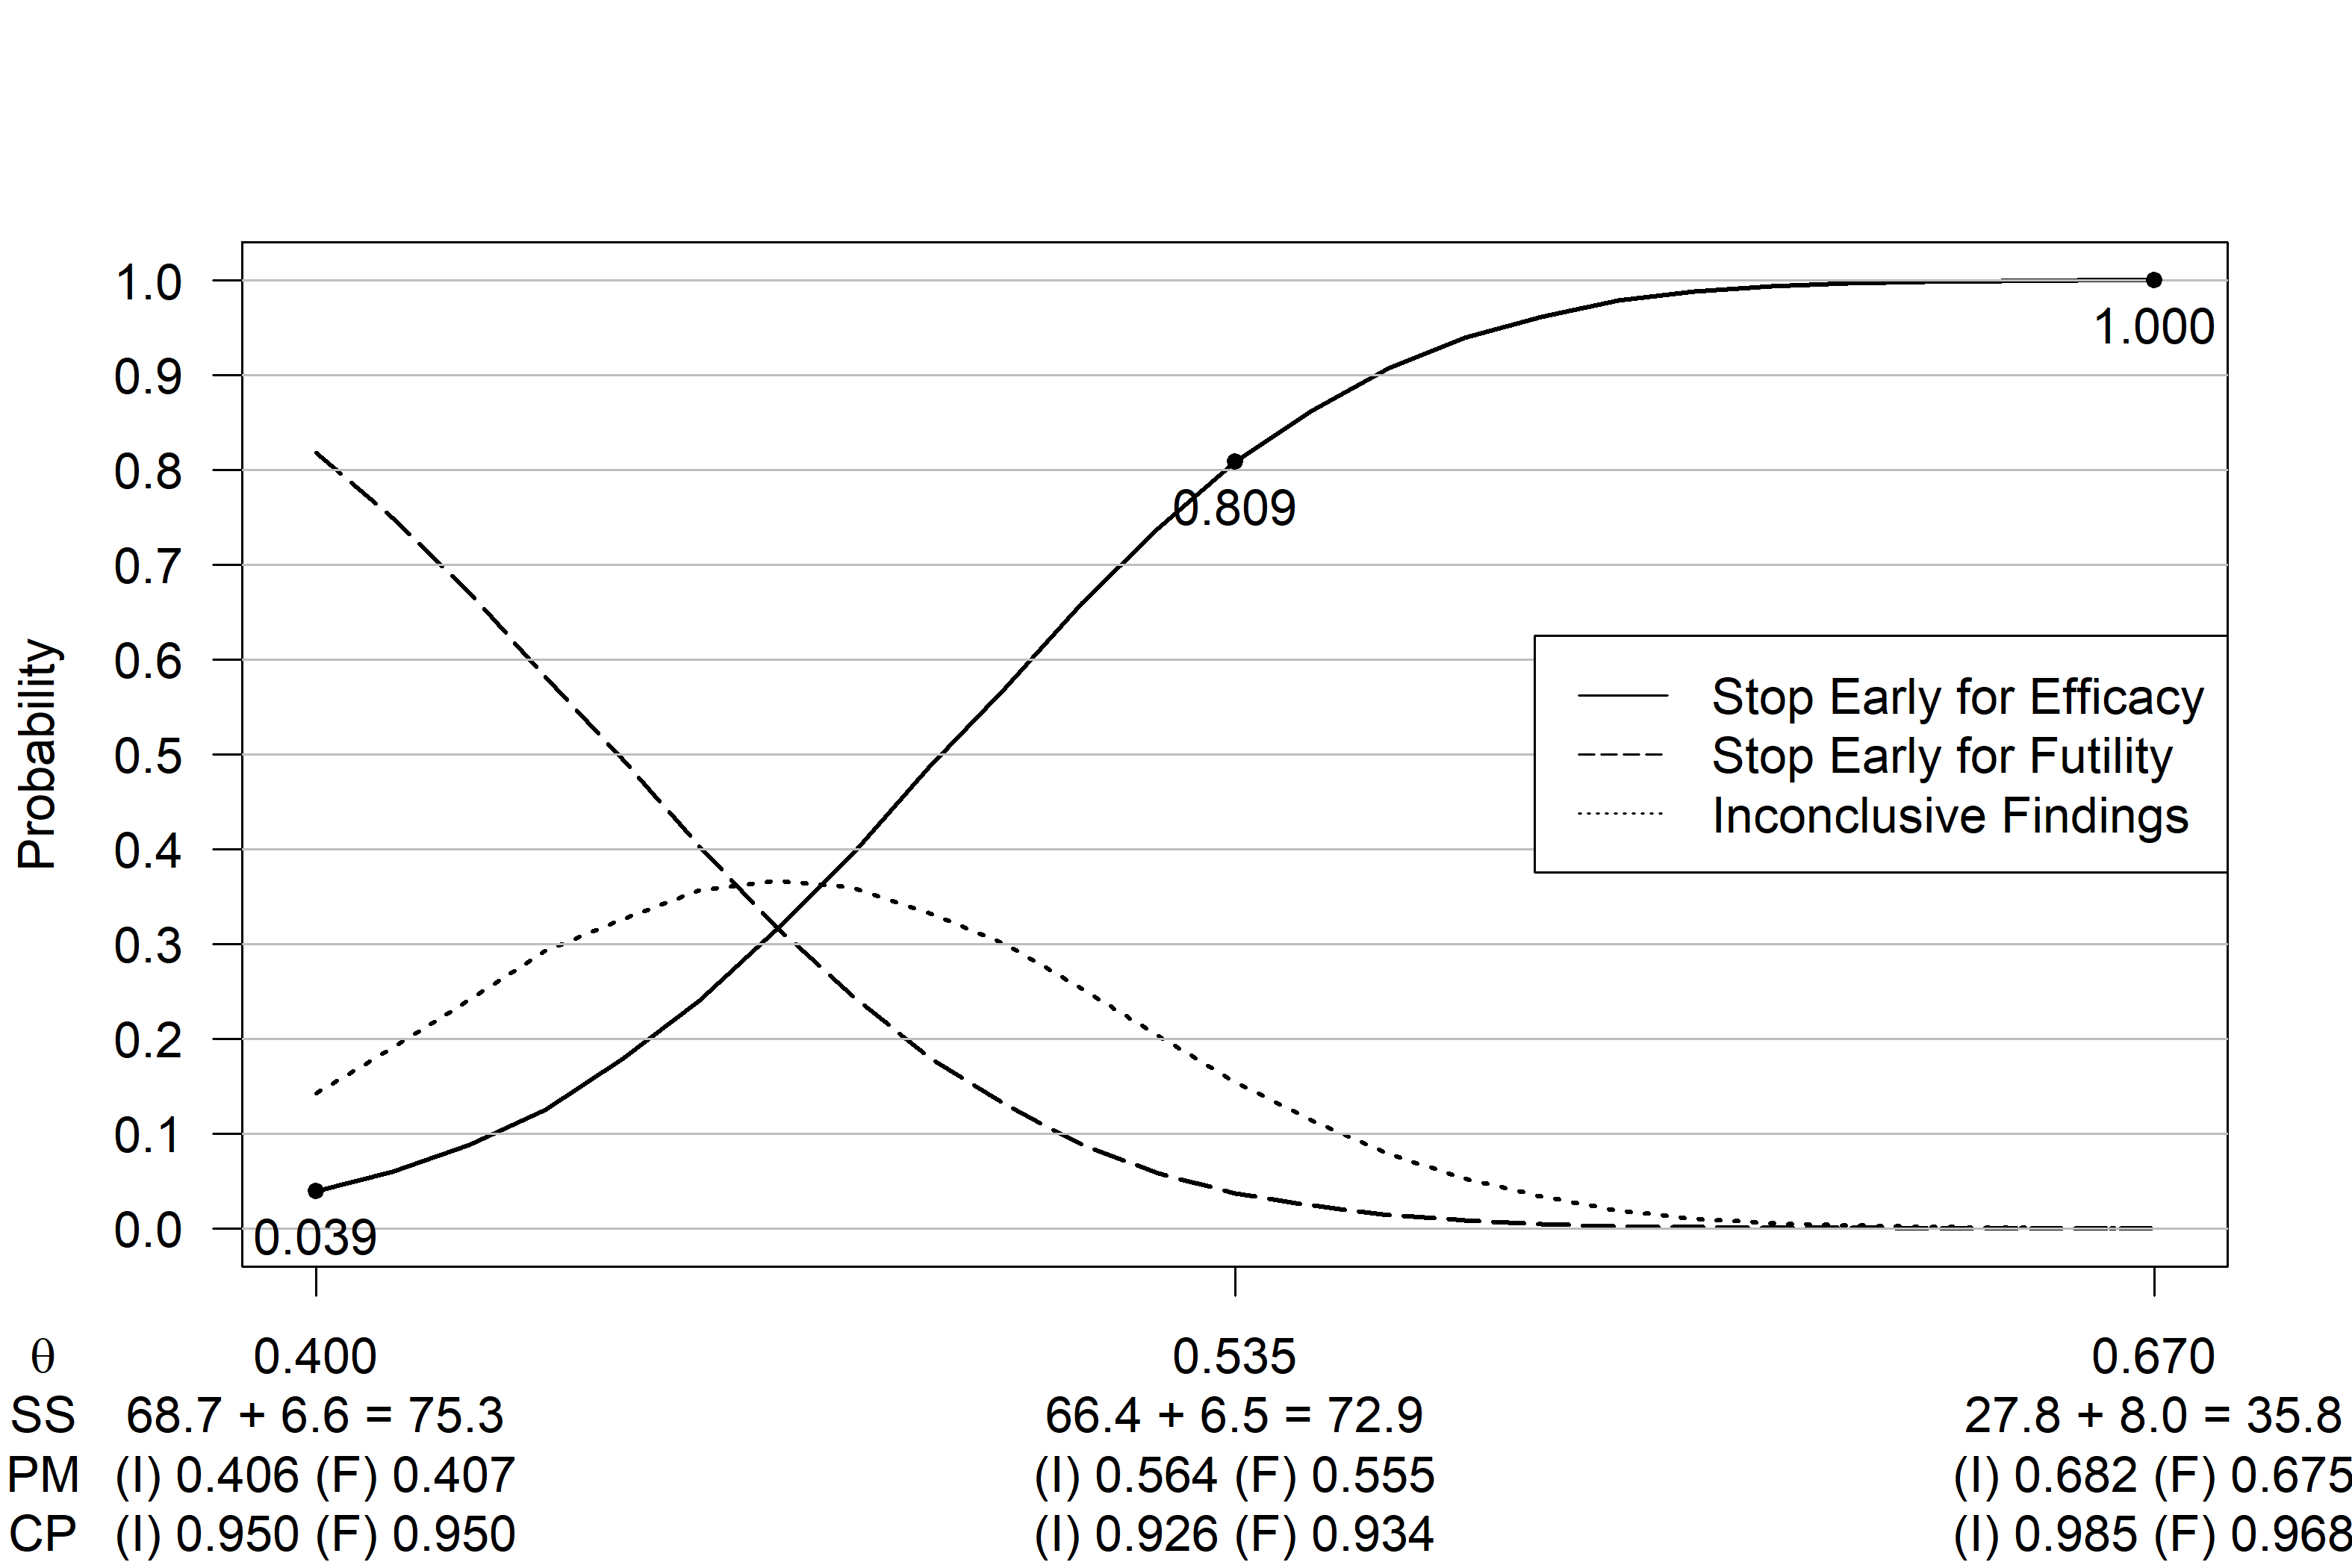
\includegraphics[width=6in]{figureS2b.png}
 \caption{Modification of enthusiastic prior parameterization in Example \ref{sec:example1}. A, default enthusiastic prior (Figure \ref{fig:figure1}(c)). B, flattened enthusiastic prior (Figure \ref{fig:figure1}(d)). Both designs use concentrated skeptical prior (Figure \ref{fig:figure1}(b)).}
\label{fig:robustness1}
\end{center}
\end{figure}
\begin{figure}\begin{center}

 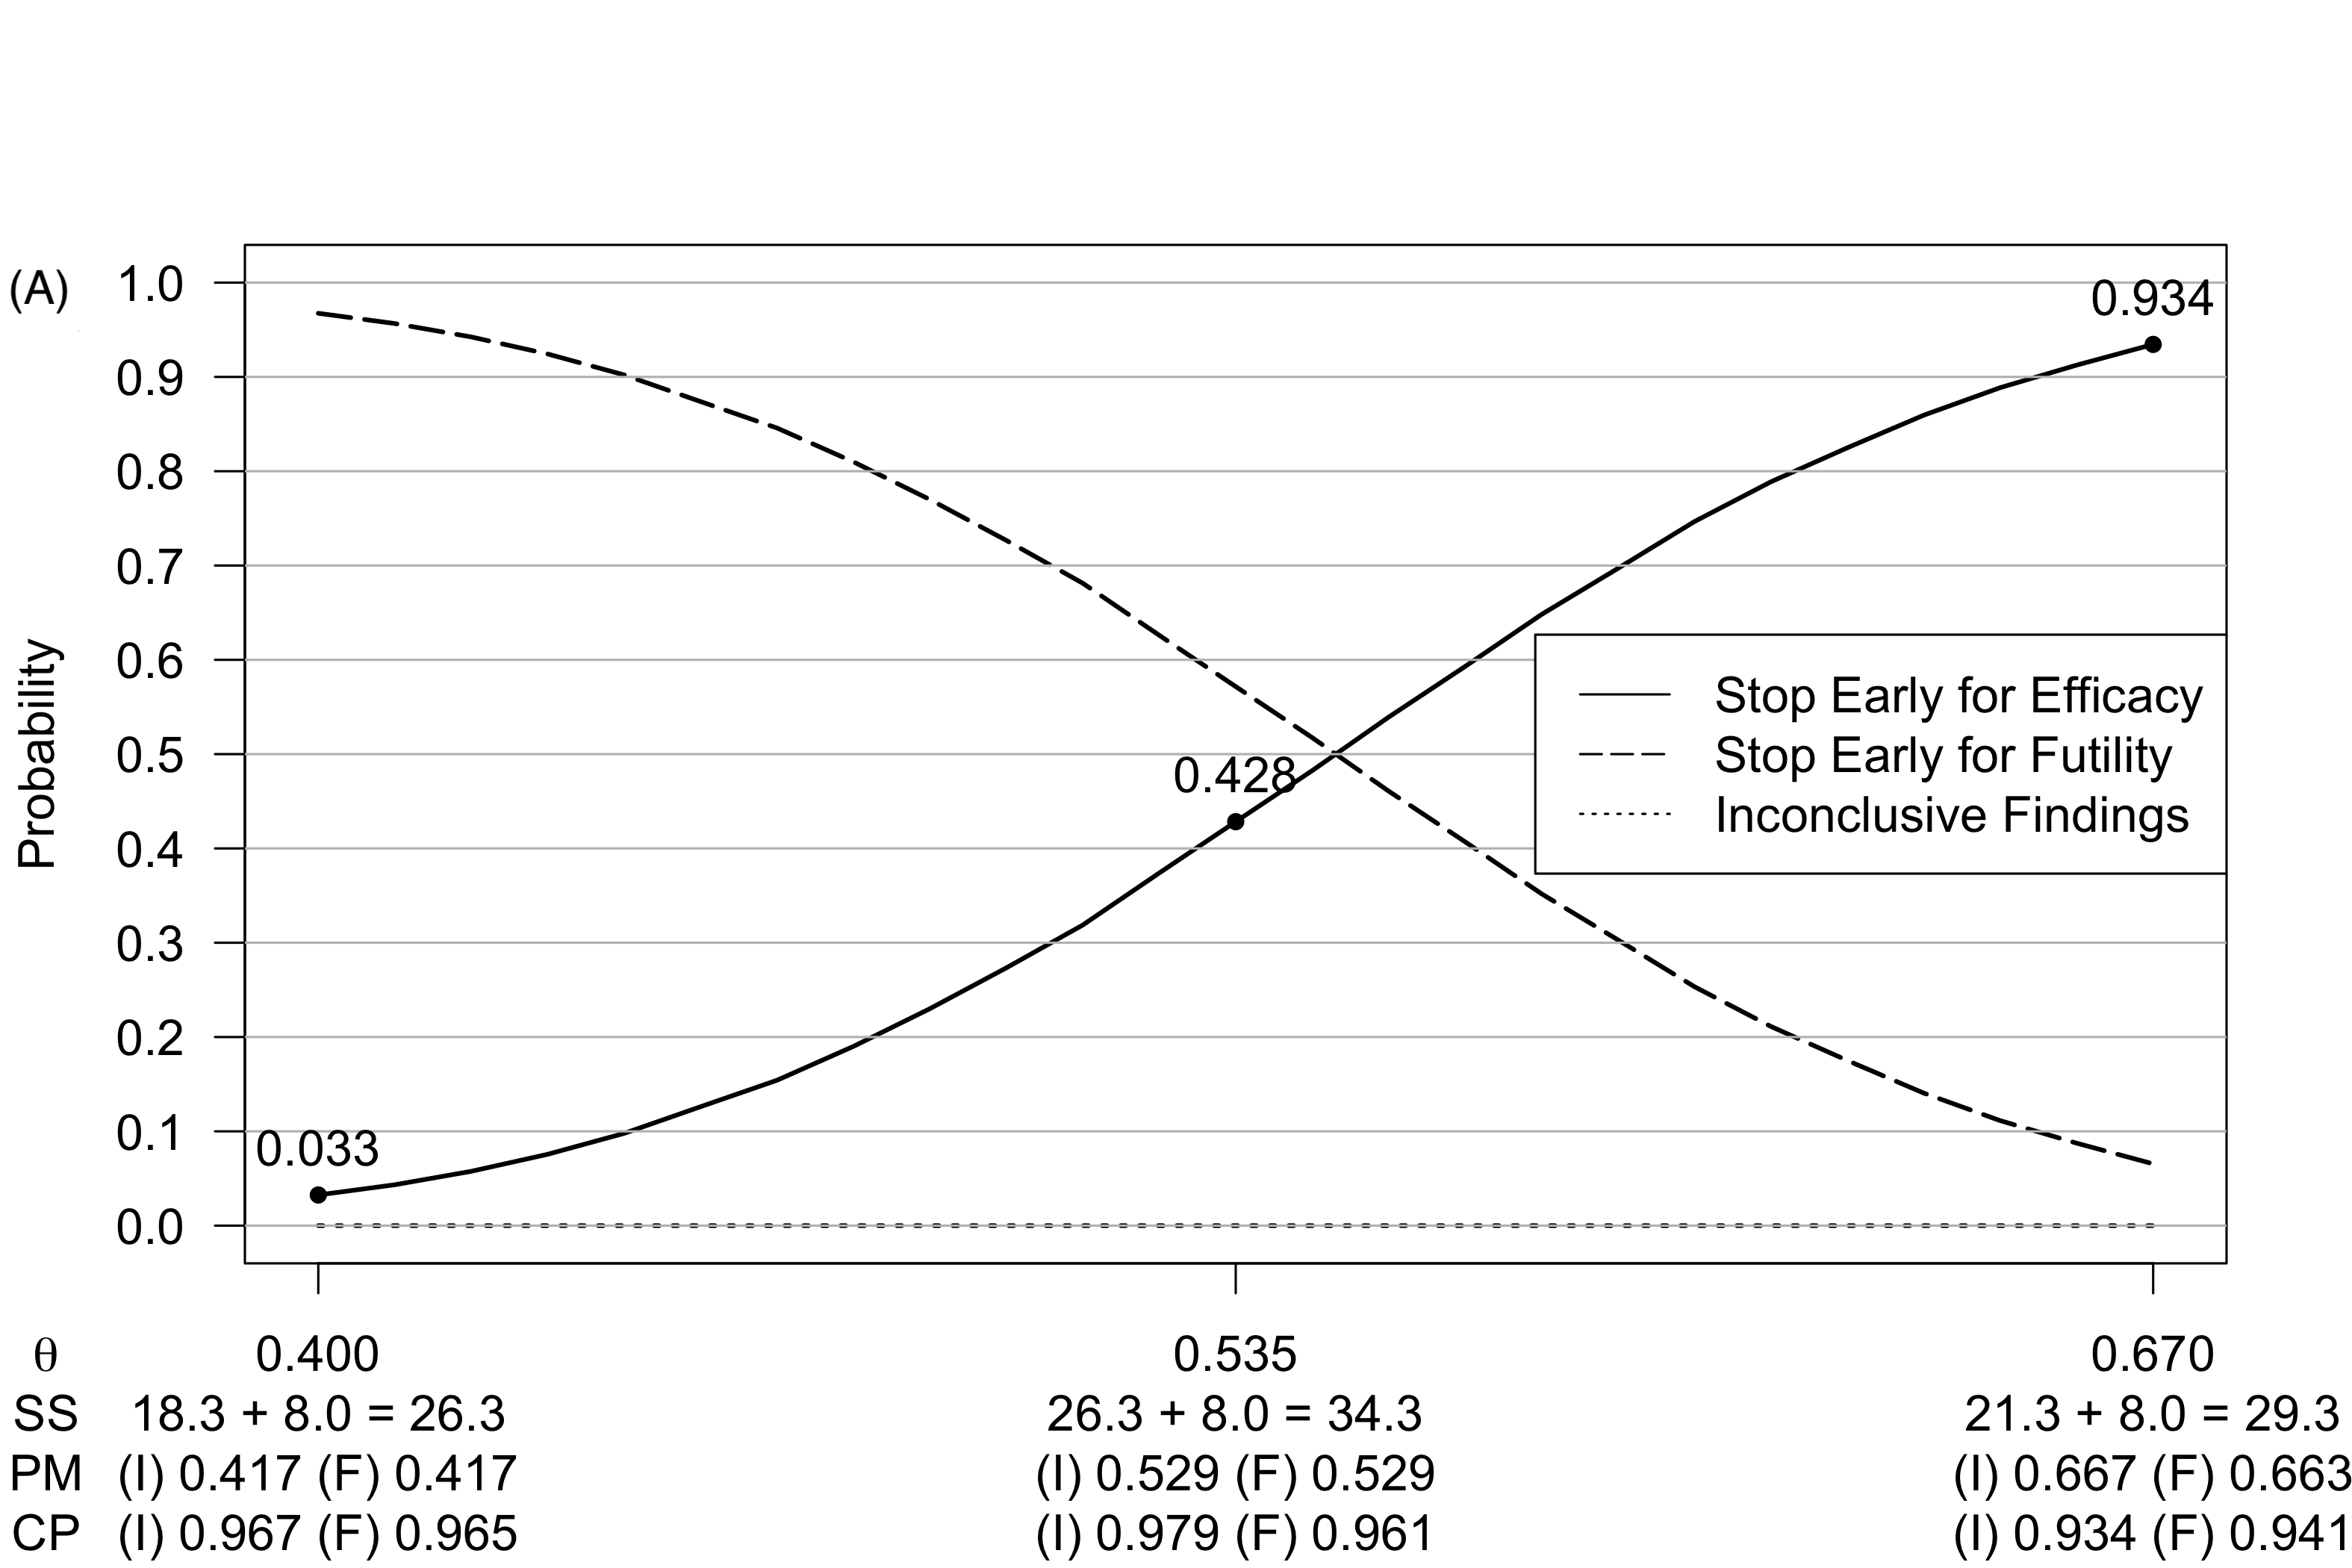
\includegraphics[width=6in]{figureS2c.png}
 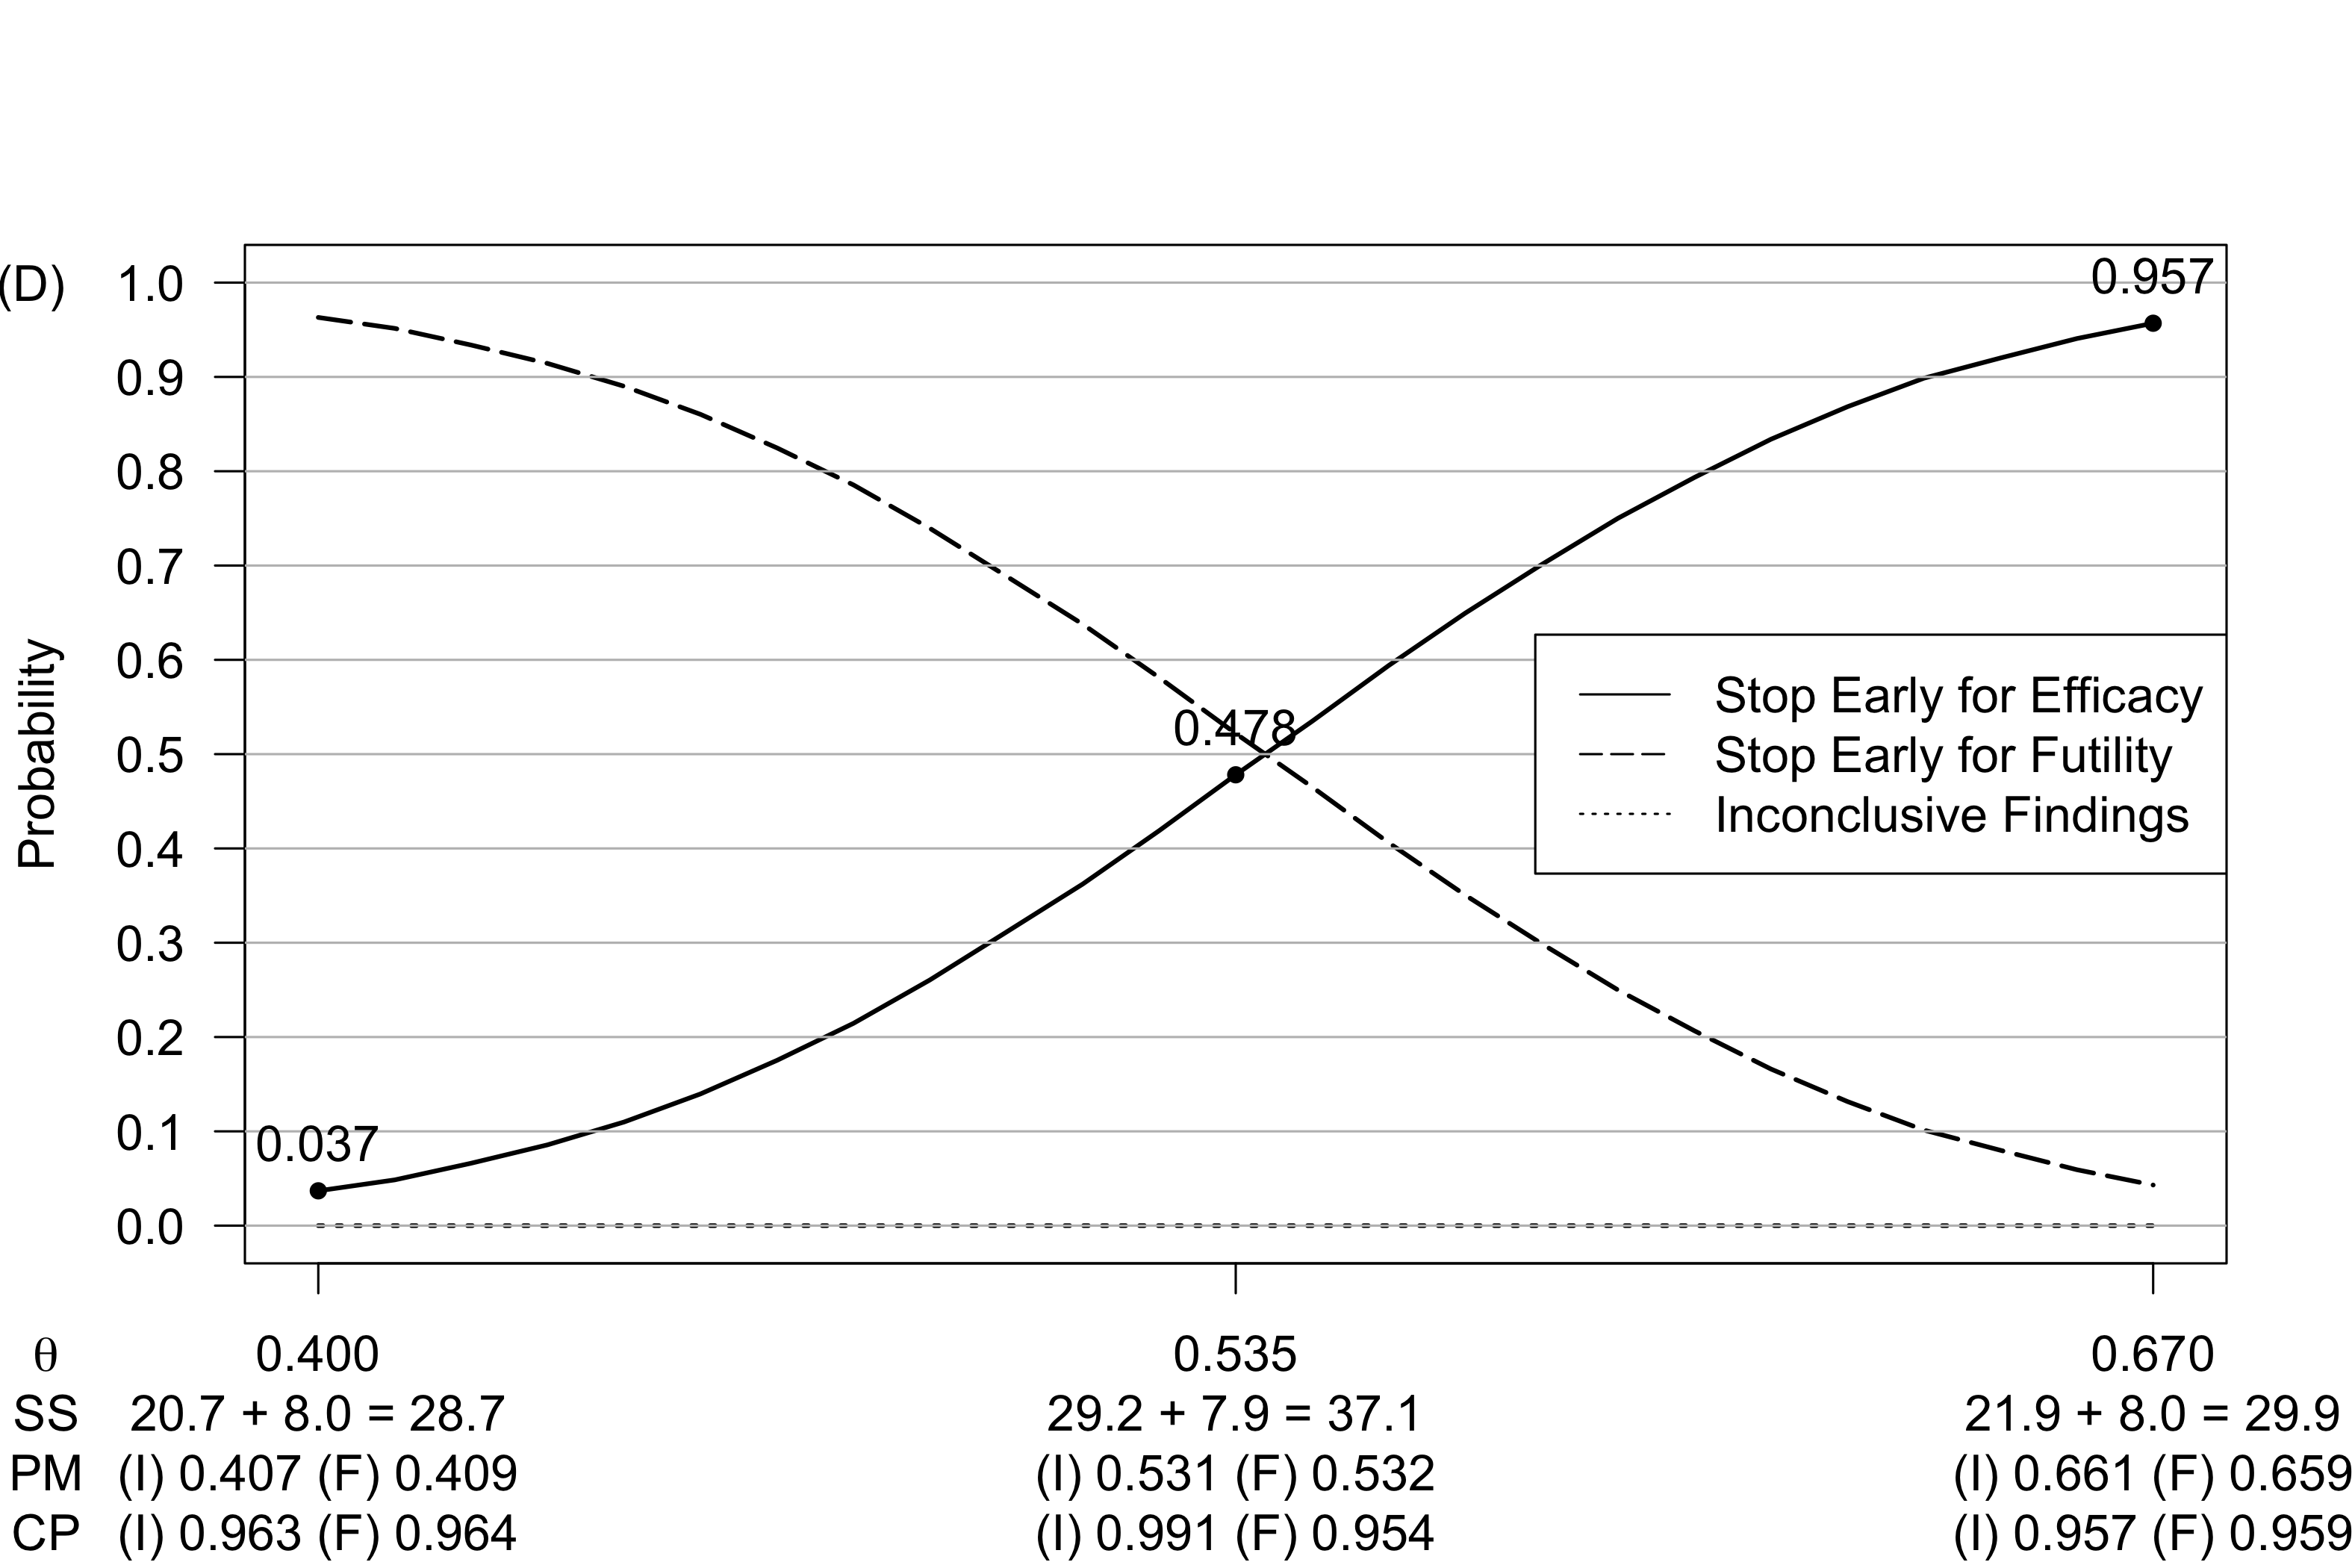
\includegraphics[width=6in]{figureS2d.png}
 \caption{Modification of enthusiastic prior parameterization in Example \ref{sec:example1}. A, default enthusiastic prior (Figure \ref{fig:figure1}(c)). B, flattened enthusiastic prior (Figure \ref{fig:figure1}(d)). Both designs use default skeptical prior (Figure \ref{fig:figure1}(a)).}
\label{fig:robustness2}
\end{center}
\end{figure}

%% latex table generated in R 4.0.0 by xtable 1.8-4 package
% Tue Jul 14 12:05:34 2020
\begin{table}[ht]
\centering
\begin{tabular}{llrrrr}
  \hline
  \hline
0.4 & FUT INITIAL & 0.7572 & 0.7653 & 0.8069 & 0.8183 \\ 
   & FUT FINAL & 0.5862 & 0.5930 & 0.6371 & 0.6455 \\ 
   & SS & 71.0198 & 73.0444 & 66.6849 & 68.6982 \\ 
  0.535 & FUT INITIAL & 0.0260 & 0.0251 & 0.0384 & 0.0370 \\ 
   & FUT FINAL & 0.0137 & 0.0127 & 0.0199 & 0.0193 \\ 
   & SS & 56.8978 & 66.8005 & 56.1953 & 66.4028 \\ 
  0.67 & FUT INITIAL & 0.0000 & 0.0000 & 0.0000 & 0.0000 \\ 
   & FUT FINAL & 0.0000 & 0.0000 & 0.0000 & 0.0000 \\ 
   & SS & 22.9456 & 27.8308 & 23.0299 & 27.8094 \\ 
   \hline
\end{tabular}
\end{table}


\label{lastpage}

\end{document}